% Options for packages loaded elsewhere
\PassOptionsToPackage{unicode}{hyperref}
\PassOptionsToPackage{hyphens}{url}
\PassOptionsToPackage{dvipsnames,svgnames,x11names}{xcolor}
%
\documentclass[
  letterpaper,
  DIV=11,
  numbers=noendperiod,
  oneside]{scrreprt}

\usepackage{amsmath,amssymb}
\usepackage{iftex}
\ifPDFTeX
  \usepackage[T1]{fontenc}
  \usepackage[utf8]{inputenc}
  \usepackage{textcomp} % provide euro and other symbols
\else % if luatex or xetex
  \usepackage{unicode-math}
  \defaultfontfeatures{Scale=MatchLowercase}
  \defaultfontfeatures[\rmfamily]{Ligatures=TeX,Scale=1}
\fi
\usepackage{lmodern}
\ifPDFTeX\else  
    % xetex/luatex font selection
\fi
% Use upquote if available, for straight quotes in verbatim environments
\IfFileExists{upquote.sty}{\usepackage{upquote}}{}
\IfFileExists{microtype.sty}{% use microtype if available
  \usepackage[]{microtype}
  \UseMicrotypeSet[protrusion]{basicmath} % disable protrusion for tt fonts
}{}
\makeatletter
\@ifundefined{KOMAClassName}{% if non-KOMA class
  \IfFileExists{parskip.sty}{%
    \usepackage{parskip}
  }{% else
    \setlength{\parindent}{0pt}
    \setlength{\parskip}{6pt plus 2pt minus 1pt}}
}{% if KOMA class
  \KOMAoptions{parskip=half}}
\makeatother
\usepackage{xcolor}
\usepackage[left=1in,marginparwidth=2.0666666666667in,textwidth=4.1333333333333in,marginparsep=0.3in]{geometry}
\setlength{\emergencystretch}{3em} % prevent overfull lines
\setcounter{secnumdepth}{5}
% Make \paragraph and \subparagraph free-standing
\makeatletter
\ifx\paragraph\undefined\else
  \let\oldparagraph\paragraph
  \renewcommand{\paragraph}{
    \@ifstar
      \xxxParagraphStar
      \xxxParagraphNoStar
  }
  \newcommand{\xxxParagraphStar}[1]{\oldparagraph*{#1}\mbox{}}
  \newcommand{\xxxParagraphNoStar}[1]{\oldparagraph{#1}\mbox{}}
\fi
\ifx\subparagraph\undefined\else
  \let\oldsubparagraph\subparagraph
  \renewcommand{\subparagraph}{
    \@ifstar
      \xxxSubParagraphStar
      \xxxSubParagraphNoStar
  }
  \newcommand{\xxxSubParagraphStar}[1]{\oldsubparagraph*{#1}\mbox{}}
  \newcommand{\xxxSubParagraphNoStar}[1]{\oldsubparagraph{#1}\mbox{}}
\fi
\makeatother

\usepackage{color}
\usepackage{fancyvrb}
\newcommand{\VerbBar}{|}
\newcommand{\VERB}{\Verb[commandchars=\\\{\}]}
\DefineVerbatimEnvironment{Highlighting}{Verbatim}{commandchars=\\\{\}}
% Add ',fontsize=\small' for more characters per line
\usepackage{framed}
\definecolor{shadecolor}{RGB}{241,243,245}
\newenvironment{Shaded}{\begin{snugshade}}{\end{snugshade}}
\newcommand{\AlertTok}[1]{\textcolor[rgb]{0.68,0.00,0.00}{#1}}
\newcommand{\AnnotationTok}[1]{\textcolor[rgb]{0.37,0.37,0.37}{#1}}
\newcommand{\AttributeTok}[1]{\textcolor[rgb]{0.40,0.45,0.13}{#1}}
\newcommand{\BaseNTok}[1]{\textcolor[rgb]{0.68,0.00,0.00}{#1}}
\newcommand{\BuiltInTok}[1]{\textcolor[rgb]{0.00,0.23,0.31}{#1}}
\newcommand{\CharTok}[1]{\textcolor[rgb]{0.13,0.47,0.30}{#1}}
\newcommand{\CommentTok}[1]{\textcolor[rgb]{0.37,0.37,0.37}{#1}}
\newcommand{\CommentVarTok}[1]{\textcolor[rgb]{0.37,0.37,0.37}{\textit{#1}}}
\newcommand{\ConstantTok}[1]{\textcolor[rgb]{0.56,0.35,0.01}{#1}}
\newcommand{\ControlFlowTok}[1]{\textcolor[rgb]{0.00,0.23,0.31}{\textbf{#1}}}
\newcommand{\DataTypeTok}[1]{\textcolor[rgb]{0.68,0.00,0.00}{#1}}
\newcommand{\DecValTok}[1]{\textcolor[rgb]{0.68,0.00,0.00}{#1}}
\newcommand{\DocumentationTok}[1]{\textcolor[rgb]{0.37,0.37,0.37}{\textit{#1}}}
\newcommand{\ErrorTok}[1]{\textcolor[rgb]{0.68,0.00,0.00}{#1}}
\newcommand{\ExtensionTok}[1]{\textcolor[rgb]{0.00,0.23,0.31}{#1}}
\newcommand{\FloatTok}[1]{\textcolor[rgb]{0.68,0.00,0.00}{#1}}
\newcommand{\FunctionTok}[1]{\textcolor[rgb]{0.28,0.35,0.67}{#1}}
\newcommand{\ImportTok}[1]{\textcolor[rgb]{0.00,0.46,0.62}{#1}}
\newcommand{\InformationTok}[1]{\textcolor[rgb]{0.37,0.37,0.37}{#1}}
\newcommand{\KeywordTok}[1]{\textcolor[rgb]{0.00,0.23,0.31}{\textbf{#1}}}
\newcommand{\NormalTok}[1]{\textcolor[rgb]{0.00,0.23,0.31}{#1}}
\newcommand{\OperatorTok}[1]{\textcolor[rgb]{0.37,0.37,0.37}{#1}}
\newcommand{\OtherTok}[1]{\textcolor[rgb]{0.00,0.23,0.31}{#1}}
\newcommand{\PreprocessorTok}[1]{\textcolor[rgb]{0.68,0.00,0.00}{#1}}
\newcommand{\RegionMarkerTok}[1]{\textcolor[rgb]{0.00,0.23,0.31}{#1}}
\newcommand{\SpecialCharTok}[1]{\textcolor[rgb]{0.37,0.37,0.37}{#1}}
\newcommand{\SpecialStringTok}[1]{\textcolor[rgb]{0.13,0.47,0.30}{#1}}
\newcommand{\StringTok}[1]{\textcolor[rgb]{0.13,0.47,0.30}{#1}}
\newcommand{\VariableTok}[1]{\textcolor[rgb]{0.07,0.07,0.07}{#1}}
\newcommand{\VerbatimStringTok}[1]{\textcolor[rgb]{0.13,0.47,0.30}{#1}}
\newcommand{\WarningTok}[1]{\textcolor[rgb]{0.37,0.37,0.37}{\textit{#1}}}

\providecommand{\tightlist}{%
  \setlength{\itemsep}{0pt}\setlength{\parskip}{0pt}}\usepackage{longtable,booktabs,array}
\usepackage{calc} % for calculating minipage widths
% Correct order of tables after \paragraph or \subparagraph
\usepackage{etoolbox}
\makeatletter
\patchcmd\longtable{\par}{\if@noskipsec\mbox{}\fi\par}{}{}
\makeatother
% Allow footnotes in longtable head/foot
\IfFileExists{footnotehyper.sty}{\usepackage{footnotehyper}}{\usepackage{footnote}}
\makesavenoteenv{longtable}
\usepackage{graphicx}
\makeatletter
\def\maxwidth{\ifdim\Gin@nat@width>\linewidth\linewidth\else\Gin@nat@width\fi}
\def\maxheight{\ifdim\Gin@nat@height>\textheight\textheight\else\Gin@nat@height\fi}
\makeatother
% Scale images if necessary, so that they will not overflow the page
% margins by default, and it is still possible to overwrite the defaults
% using explicit options in \includegraphics[width, height, ...]{}
\setkeys{Gin}{width=\maxwidth,height=\maxheight,keepaspectratio}
% Set default figure placement to htbp
\makeatletter
\def\fps@figure{htbp}
\makeatother
% definitions for citeproc citations
\NewDocumentCommand\citeproctext{}{}
\NewDocumentCommand\citeproc{mm}{%
  \begingroup\def\citeproctext{#2}\cite{#1}\endgroup}
\makeatletter
 % allow citations to break across lines
 \let\@cite@ofmt\@firstofone
 % avoid brackets around text for \cite:
 \def\@biblabel#1{}
 \def\@cite#1#2{{#1\if@tempswa , #2\fi}}
\makeatother
\newlength{\cslhangindent}
\setlength{\cslhangindent}{1.5em}
\newlength{\csllabelwidth}
\setlength{\csllabelwidth}{3em}
\newenvironment{CSLReferences}[2] % #1 hanging-indent, #2 entry-spacing
 {\begin{list}{}{%
  \setlength{\itemindent}{0pt}
  \setlength{\leftmargin}{0pt}
  \setlength{\parsep}{0pt}
  % turn on hanging indent if param 1 is 1
  \ifodd #1
   \setlength{\leftmargin}{\cslhangindent}
   \setlength{\itemindent}{-1\cslhangindent}
  \fi
  % set entry spacing
  \setlength{\itemsep}{#2\baselineskip}}}
 {\end{list}}
\usepackage{calc}
\newcommand{\CSLBlock}[1]{\hfill\break\parbox[t]{\linewidth}{\strut\ignorespaces#1\strut}}
\newcommand{\CSLLeftMargin}[1]{\parbox[t]{\csllabelwidth}{\strut#1\strut}}
\newcommand{\CSLRightInline}[1]{\parbox[t]{\linewidth - \csllabelwidth}{\strut#1\strut}}
\newcommand{\CSLIndent}[1]{\hspace{\cslhangindent}#1}

\usepackage{fvextra}
\DefineVerbatimEnvironment{Highlighting}{Verbatim}{breaklines,commandchars=\\\{\}}
\DefineVerbatimEnvironment{OutputCode}{Verbatim}{breaklines,commandchars=\\\{\}}
\KOMAoption{captions}{tableheading}
\makeatletter
\@ifpackageloaded{tcolorbox}{}{\usepackage[skins,breakable]{tcolorbox}}
\@ifpackageloaded{fontawesome5}{}{\usepackage{fontawesome5}}
\definecolor{quarto-callout-color}{HTML}{909090}
\definecolor{quarto-callout-note-color}{HTML}{0758E5}
\definecolor{quarto-callout-important-color}{HTML}{CC1914}
\definecolor{quarto-callout-warning-color}{HTML}{EB9113}
\definecolor{quarto-callout-tip-color}{HTML}{00A047}
\definecolor{quarto-callout-caution-color}{HTML}{FC5300}
\definecolor{quarto-callout-color-frame}{HTML}{acacac}
\definecolor{quarto-callout-note-color-frame}{HTML}{4582ec}
\definecolor{quarto-callout-important-color-frame}{HTML}{d9534f}
\definecolor{quarto-callout-warning-color-frame}{HTML}{f0ad4e}
\definecolor{quarto-callout-tip-color-frame}{HTML}{02b875}
\definecolor{quarto-callout-caution-color-frame}{HTML}{fd7e14}
\makeatother
\makeatletter
\@ifpackageloaded{bookmark}{}{\usepackage{bookmark}}
\makeatother
\makeatletter
\@ifpackageloaded{caption}{}{\usepackage{caption}}
\AtBeginDocument{%
\ifdefined\contentsname
  \renewcommand*\contentsname{Table of contents}
\else
  \newcommand\contentsname{Table of contents}
\fi
\ifdefined\listfigurename
  \renewcommand*\listfigurename{List of Figures}
\else
  \newcommand\listfigurename{List of Figures}
\fi
\ifdefined\listtablename
  \renewcommand*\listtablename{List of Tables}
\else
  \newcommand\listtablename{List of Tables}
\fi
\ifdefined\figurename
  \renewcommand*\figurename{Figure}
\else
  \newcommand\figurename{Figure}
\fi
\ifdefined\tablename
  \renewcommand*\tablename{Table}
\else
  \newcommand\tablename{Table}
\fi
}
\@ifpackageloaded{float}{}{\usepackage{float}}
\floatstyle{ruled}
\@ifundefined{c@chapter}{\newfloat{codelisting}{h}{lop}}{\newfloat{codelisting}{h}{lop}[chapter]}
\floatname{codelisting}{Listing}
\newcommand*\listoflistings{\listof{codelisting}{List of Listings}}
\makeatother
\makeatletter
\makeatother
\makeatletter
\@ifpackageloaded{caption}{}{\usepackage{caption}}
\@ifpackageloaded{subcaption}{}{\usepackage{subcaption}}
\makeatother
\makeatletter
\@ifpackageloaded{sidenotes}{}{\usepackage{sidenotes}}
\@ifpackageloaded{marginnote}{}{\usepackage{marginnote}}
\makeatother
\ifLuaTeX
  \usepackage{selnolig}  % disable illegal ligatures
\fi
\usepackage{bookmark}

\IfFileExists{xurl.sty}{\usepackage{xurl}}{} % add URL line breaks if available
\urlstyle{same} % disable monospaced font for URLs
\hypersetup{
  pdftitle={Data Literacy for the Language Sciences},
  pdfauthor={Elen Le Foll},
  colorlinks=true,
  linkcolor={blue},
  filecolor={Maroon},
  citecolor={Blue},
  urlcolor={Blue},
  pdfcreator={LaTeX via pandoc}}

\title{Data Literacy for the Language Sciences}
\usepackage{etoolbox}
\makeatletter
\providecommand{\subtitle}[1]{% add subtitle to \maketitle
  \apptocmd{\@title}{\par {\large #1 \par}}{}{}
}
\makeatother
\subtitle{A very gentle introduction to statistics and data
visualisation in R}
\author{Elen Le Foll}
\date{2024-05-06}

\begin{document}
\maketitle

\renewcommand*\contentsname{Table of contents}
{
\hypersetup{linkcolor=}
\setcounter{tocdepth}{2}
\tableofcontents
}
\bookmarksetup{startatroot}

\chapter*{Preface}\label{preface}
\addcontentsline{toc}{chapter}{Preface}

\markboth{Preface}{Preface}

\begin{tcolorbox}[enhanced jigsaw, breakable, colbacktitle=quarto-callout-warning-color!10!white, bottomtitle=1mm, colframe=quarto-callout-warning-color-frame, leftrule=.75mm, bottomrule=.15mm, colback=white, toptitle=1mm, rightrule=.15mm, title=\textcolor{quarto-callout-warning-color}{\faExclamationTriangle}\hspace{0.5em}{Warning}, coltitle=black, opacityback=0, arc=.35mm, left=2mm, titlerule=0mm, toprule=.15mm, opacitybacktitle=0.6]

This textbook draft is very much \textbf{work in progress}. I intend to
progressively add to it over the course of the summer semester 2024.
Note that the PDF version is not optimised in any way. For now, I
recommend only looking at the web-book version available on:
\url{https://elenlefoll.github.io/RstatsTextbook/}.

This first draft is intended as complementary materials to my M.A.~class
``More than counting words: Introduction to statistics and data
visualisation for linguists'', which I teach at the University of
Cologne.

Student feedback on this first draft is very welcome!

\end{tcolorbox}

\section*{Who is this book for?}\label{who-is-this-book-for}
\addcontentsline{toc}{section}{Who is this book for?}

\markright{Who is this book for?}

This textbook is intended as a very gentle introduction to basic
principles of data literacy, statistics, and data visualisation using
the programming language and environment \texttt{R}. The target audience
are students and researchers in the language sciences, including
(applied) linguistics, (first and second) language teaching, and
language education research. The rationale for this textbook is based on
my personal observations, in teaching and consulting both students and
researcher colleagues, that many `introductory' textbooks assume
previous knowledge and skills that not all have or go through contents
at too fast a pace for many humanities scholars who often come with
little to no experience with programming and/or statistics.

The aim of this textbook is by no means to replace any of the brilliant
existing textbooks aimed at imparting statistical literacy for
linguistics research, but rather to provide a stepping stone towards
being able to make the most of these wonderful existing resources. A
(work-in-progress) list of next-step resources is included in
\href{https://elenlefoll.github.io/RstatsTextbook/FurtherResources.html}{Appendix
A}.

\begin{figure}

\centering{

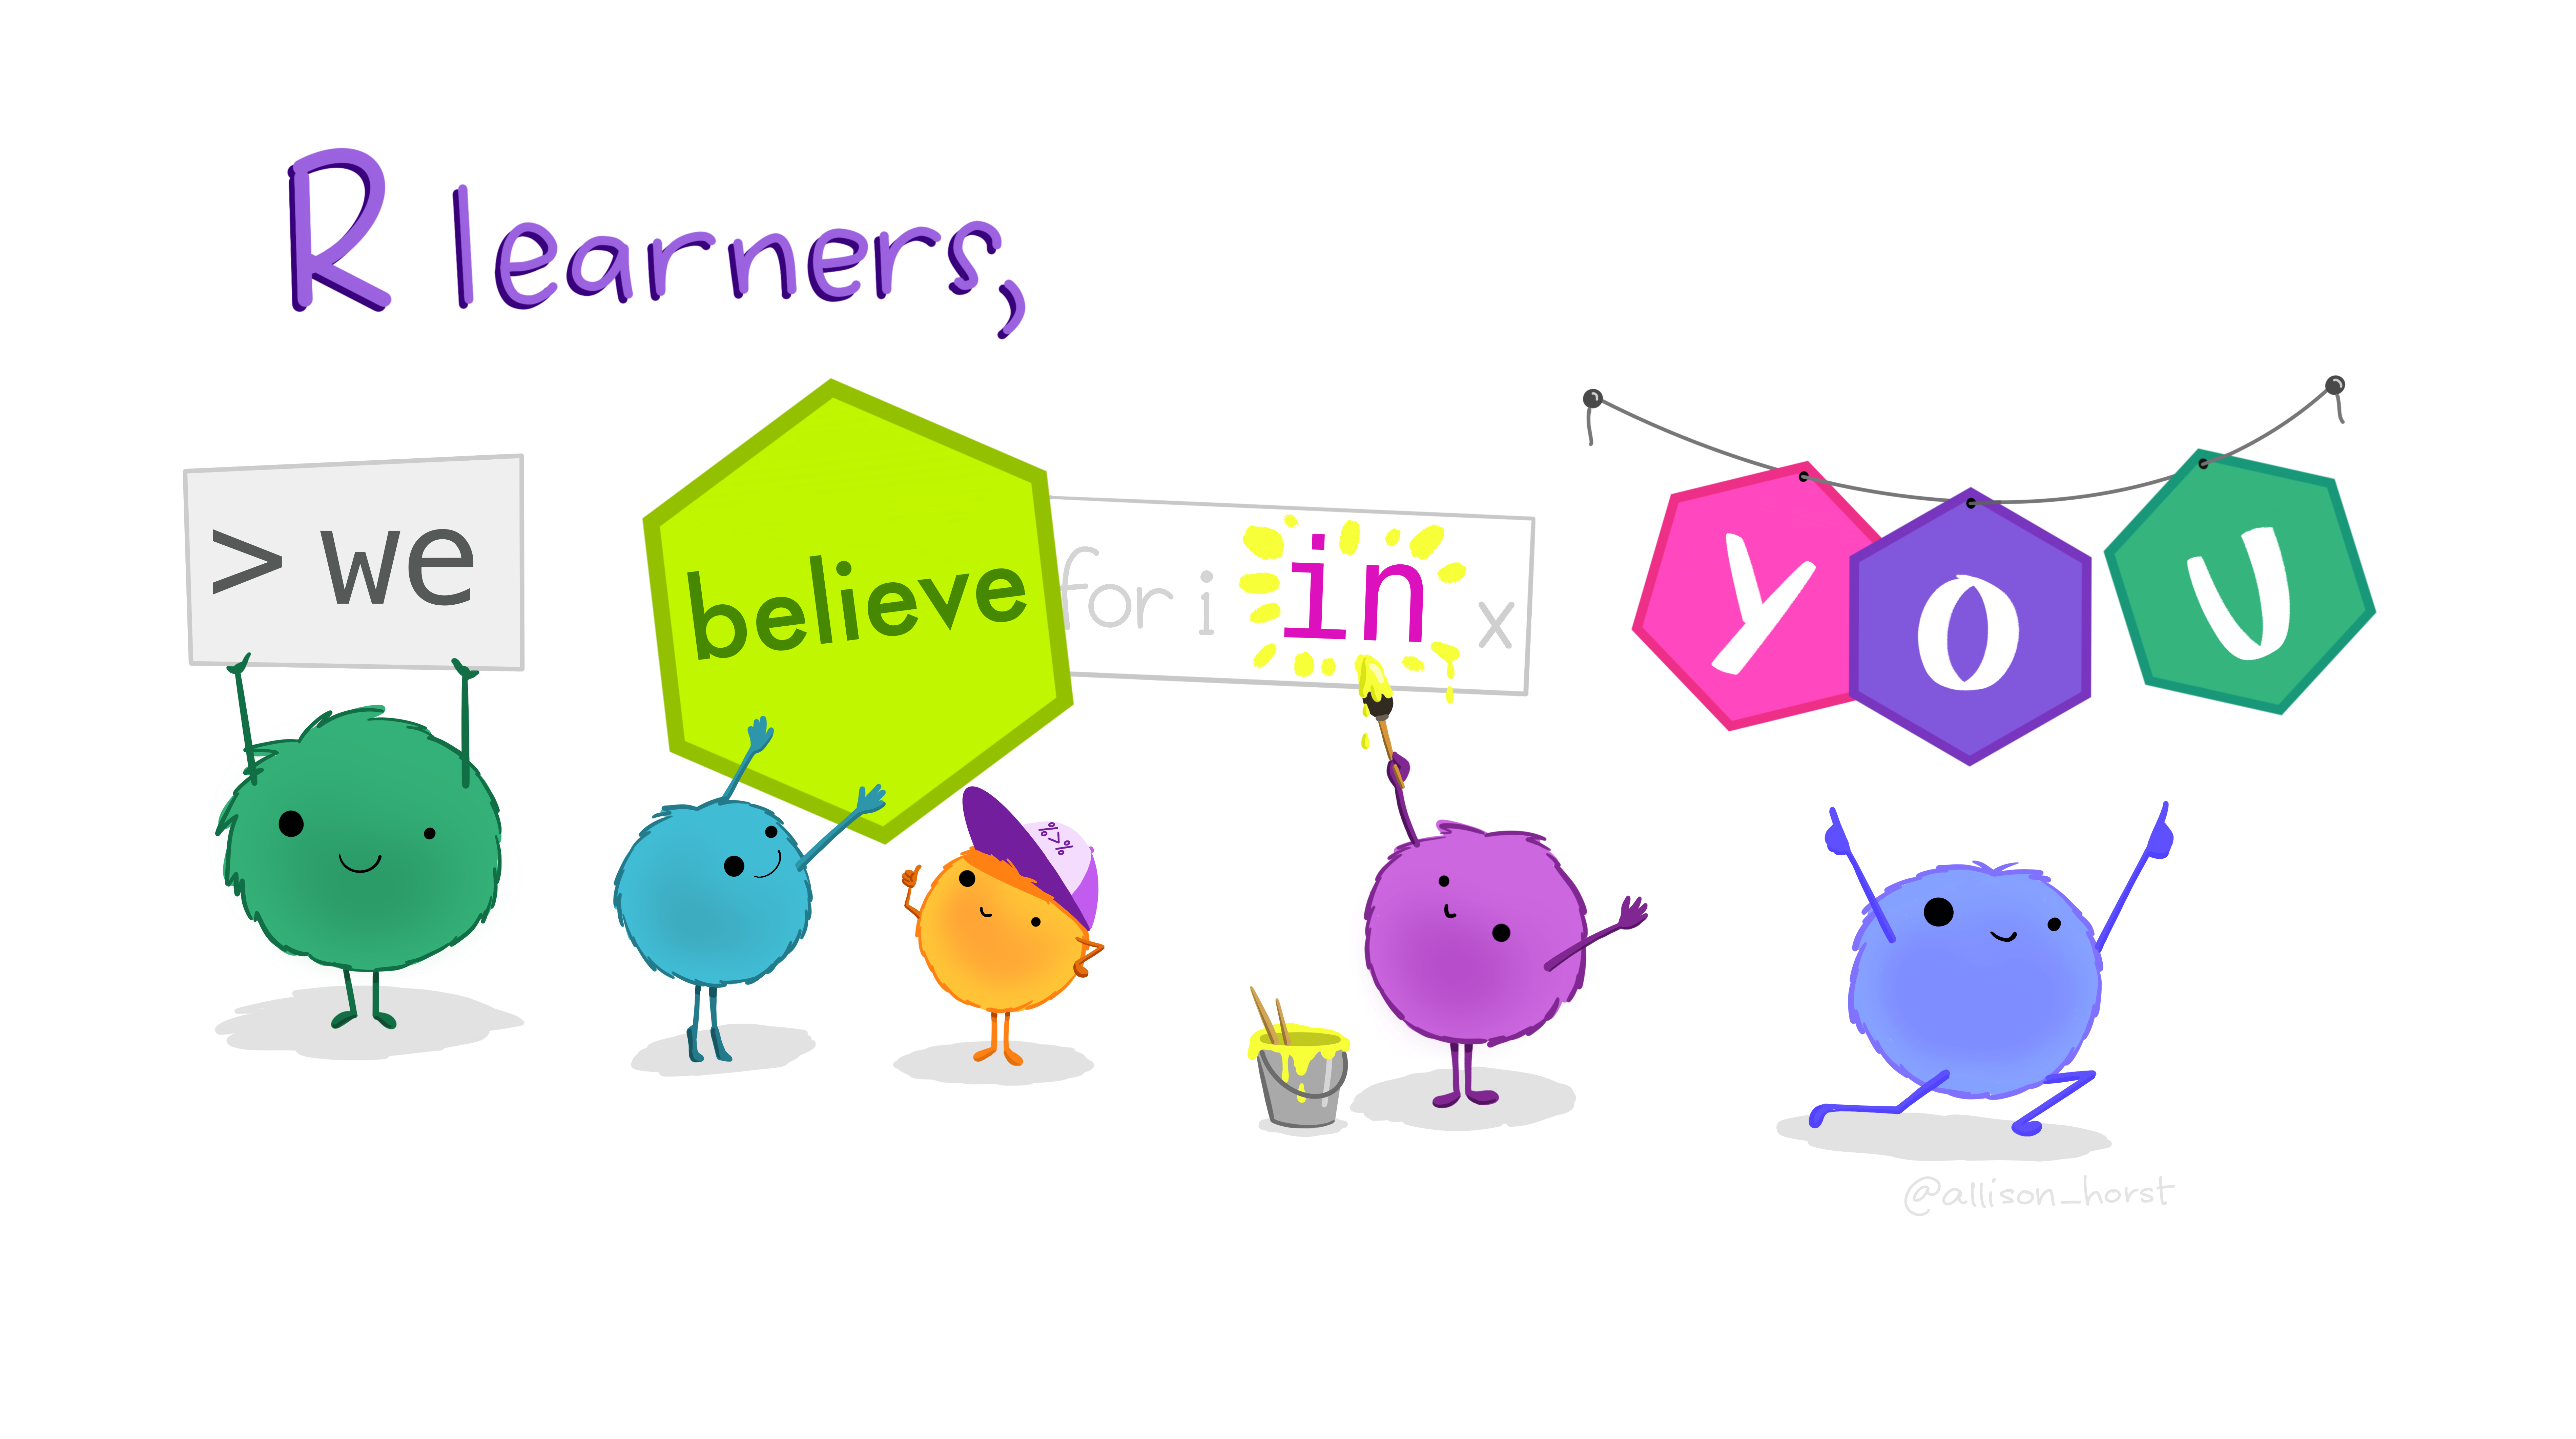
\includegraphics{images/RLearnersWeBelieve.png}

}

\caption{\label{fig-WeBelieveinYou}Artwork encouraging beginner
\texttt{R} learners by
\href{https://allisonhorst.com/allison-horst}{@allison\_horst}}

\end{figure}%

\bookmarksetup{startatroot}

\chapter{Open Scholarship}\label{open-scholarship}

This book aims to provide a stepping stone for students and scholars of
traditionally less quantitative and computational disciplines (such as
some branches of linguistics and language education research) to gather
first (hopefully positive!) experiences with statistical and
computational approaches to working with empirical data\footnote{Emprical
  data is based on what is experienced or observed rather than on theory
  alone.}. The underlying belief is that these methods ought to be
accessible to all, regardless of their academic background or personal
circumstances. To this end, this book embraces the principles of Open
Scholarship.

Open Scholarship ``reflects the idea that knowledge of all kinds should
be openly shared, transparent, rigorous, reproducible, replicable,
accumulative, and inclusive (allowing for all knowledge systems)''
(Parsons et al. 2022). For this to be the case, teaching materials need
to shared openly and the tools and software taught in these resources
need to be freely accessible, too. In the following, we will briefly
consider the role of Open Educational Resources (OERs) and open-source
software in our pursuit of Open Scholarship.

\section{Open Source}\label{open-source}

In line with its aim to provide an accessible introduction to statistics
and data visualisation, this textbook relies exclusively on open-source
software and programming languages, foremost \texttt{LibreOffice\ Calc},
\texttt{R} and \texttt{RStudio}. Open source refers to software whose
source code is available under a license that grants anyone the rights
to study, modify, and distribute the software to anyone and for any
purpose. If we think of a software application as a cake, the source
code is like its recipe. It contains the list of ingredients and the
steps to bake the cake. Open source means that the recipe is publicly
available. You can access it, read it, and use it to bake the cake. You
can also modify it to add your own twist, such as adding a new
ingredient or making it vegan, and share it with others. In the context
of software, this allows many people to collaborate, make improvements,
and share their versions, resulting in better and more diverse software.

Using open-source software in this introductory textbook means that
anyone\footnote{Provided that they have access to the internet and a
  functioning personal computer.} can download, install and use the
required software at no cost. However, it is very important to note that
not all free software (\emph{freeware}) is open source. Let us
illustrate the difference by comparing different spreadsheet programmes
as, in the following chapter, we will begin exploring tabular data
structures in a spreadsheet programme.

The most most widely used spreadsheet programme to date is undoubtedly
\texttt{Microsoft\ Excel}. Excel is a commercial, proprietary
spreadsheet editor which forms part of the Microsoft 365 package. As
such, to use Excel on your personal computer, you need to buy a license
or be a member of an organisation (e.g., your university or company)
that pays for such a license. It is true that Microsoft now also offers
a free (functionally limited) web-based version of Excel, yet this still
does not make it open source. This is because Microsoft does not share
the source code of any Excel version, which means that, even if they are
giving away free cake, we do not have the recipe to bake the cake
ourselves should the company decide to start charging money for the cake
or to no longer distribute it at all! Similarly, you may be familiar
with a popular, web-based alternative to Excel: \texttt{Google\ Sheets}.
Whilst it is (currently) free to use, as the name suggests, Google
Sheets is owned by Google and is therefore not open source, either. By
contrast, \texttt{LibreOffice\ Calc} is a project of The Document
Foundation (TDF) that provides a popular, free, open-source office
productivity software suite comparable to Microsoft 365 called
\texttt{LibreOffice}. LibreOffice is developed collaboratively by very
many different people across the world who all do so on a volunteer
basis. The Document Foundation estimates that there are 200 million
active LibreOffice users worldwide, about 25\% of whom are thought to be
students (figures from 2018, see LibreOffice 2024). Its popularity is
likely due to the fact that it not only uses open formats (e.g.,
\texttt{.odt} and \texttt{.ods}), but can also open and save to a range
of popular formats including those used by Microsoft (e.g.,
\texttt{.docx} and \texttt{.xlsx}).

\begin{quote}
\section*{Quiz time!}\label{quiz-time}
\addcontentsline{toc}{section}{Quiz time!}

\markright{Quiz time!}

1) Which of these is an open-source alternative to Microsoft Word?

~

2) Which of these is an open-source alternative to Microsoft Powerpoint?

~

3) Not only can software be open source, programming languages can, too.
In fact, most modern programming languages are open source. In this
book, we will focus on the open-source programming language \texttt{R}.
Which of these is \emph{not} an open-source programming language?

~

4) There are also many open-source operating systems. Which of these is
an open-source alternative to the operating system Windows?

~
\end{quote}

\begin{tcolorbox}[enhanced jigsaw, breakable, colbacktitle=quarto-callout-caution-color!10!white, bottomtitle=1mm, colframe=quarto-callout-caution-color-frame, leftrule=.75mm, bottomrule=.15mm, colback=white, toptitle=1mm, rightrule=.15mm, title=\textcolor{quarto-callout-caution-color}{\faFire}\hspace{0.5em}{Task 1}, coltitle=black, opacityback=0, arc=.35mm, left=2mm, titlerule=0mm, toprule=.15mm, opacitybacktitle=0.6]

Your first task is to \textbf{download} and \textbf{install}
\textbf{LibreOffice} as we will use its spreadsheet editor,
\textbf{LibreOffice Calc}, in the next few chapters.

\begin{itemize}
\item
  LibreOffice is available for Windows, Mac and Linux. You can download
  it from here:
  \url{https://www.libreoffice.org/download/download-libreoffice/.}
\item
  You will find detailed installation instructions here:
  \href{https://www.libreoffice.org/get-help/install-howto/.You}{https://www.libreoffice.org/get-help/install-howto/.}
\item
  Detailed documentation is also available in many different languages:
  \url{https://documentation.libreoffice.org/en/english-documentation/}
\end{itemize}

\end{tcolorbox}

\section{Open Education}\label{open-education}

The web-based version of this textbook is published as an Open
Educational Resource (OER; see Figure~\ref{fig-OER}) under the Creative
Commons license:
\href{https://creativecommons.org/licenses/by-nc-sa/4.0/}{\texttt{CC\ BY-NC-SA}}.
This means that it is free to read and use, as well as edit, remix, and
expand upon, provided that:

\begin{enumerate}
\def\labelenumi{\arabic{enumi}.}
\item
  the original author and source is mentioned (as indicated by
  \href{https://creativecommons.org/licenses/by-nc-sa/4.0/}{\texttt{BY}}),
\item
  any derived version is not made into a commercial product
  (\href{https://creativecommons.org/licenses/by-nc-sa/4.0/}{\texttt{NC}}
  stands for n\emph{on-commercial}), and that
\item
  any derived versions of this textbook (e.g., a translated version or a
  version adapted for history scholars) are also shared with this same
  license
  (\href{https://creativecommons.org/licenses/by-nc-sa/4.0/}{\texttt{SA}}
  stands for \emph{share alike}).
\end{enumerate}

In line with the principles of Open Education, all of the datasets that
we will work with in this textbook have been published in Open Access,
which means that we can freely use them to learn about statistics and
data visualisation using real datasets from published research studies
in applied linguistics and language education.

\begin{figure}

\centering{

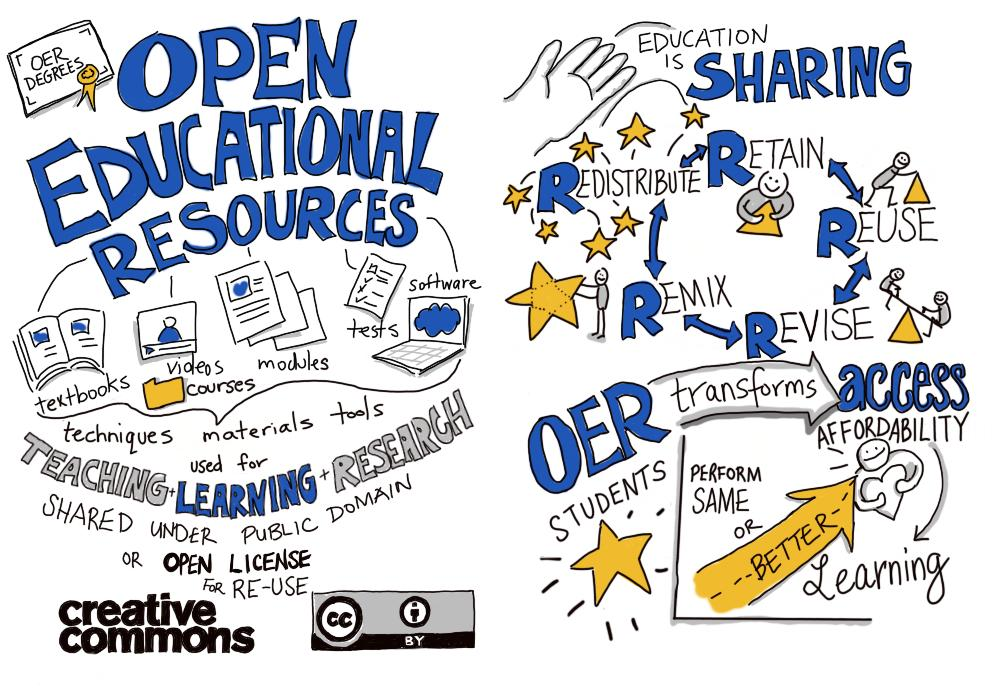
\includegraphics{images/oer.jpg}

}

\caption{\label{fig-OER}OER sketch note by
\href{https://leko.th-nuernberg.de/portal_digitale_lehre/praxisbeispiele/lehrmaterialien-teilen-fuer-flexibles-lernen/}{Yvonne
Stry}}

\end{figure}%

\begin{tcolorbox}[enhanced jigsaw, breakable, colbacktitle=quarto-callout-note-color!10!white, bottomtitle=1mm, colframe=quarto-callout-note-color-frame, leftrule=.75mm, bottomrule=.15mm, colback=white, toptitle=1mm, rightrule=.15mm, title=\textcolor{quarto-callout-note-color}{\faInfo}\hspace{0.5em}{Tips to go further}, coltitle=black, opacityback=0, arc=.35mm, left=2mm, titlerule=0mm, toprule=.15mm, opacitybacktitle=0.6]

This chapter has simplified things considerably. To be considered open
source, software distributions actually have to comply with ten
criteria. You can read up on them here:

\begin{itemize}
\tightlist
\item
  \url{https://opensource.org/osd}
\end{itemize}

To find out more about the benefits of open-source software in the
context of research, I recommend reading:

\begin{itemize}
\tightlist
\item
  \url{https://book.the-turing-way.org/reproducible-research/open/open-source}
\end{itemize}

To find out more about Open Educational Resources (OERs), I recommend
exploring the following OER databases:

\begin{itemize}
\tightlist
\item
  \url{https://oercommons.org/}
\item
  \url{https://www.twillo.de/oer/web/}
\end{itemize}

\end{tcolorbox}

\bookmarksetup{startatroot}

\chapter{Installing R and RStudio}\label{installing-r-and-rstudio}

\subsubsection*{\texorpdfstring{\textbf{Chapter
overview}}{Chapter overview}}\label{chapter-overview}
\addcontentsline{toc}{subsubsection}{\textbf{Chapter overview}}

This chapter is designed to help you get started using \texttt{R} and
\texttt{RStudio}, assuming no prior use of either. We will be covering
the following topics:

\begin{itemize}
\tightlist
\item
  Why it's worth learning \texttt{R}
\item
  Downloading \texttt{R} and \texttt{RStudio}
\item
  Setting up \texttt{RStudio}
\item
  Using the console in \texttt{RStudio}
\item
  Installing and loading \texttt{R} packages
\item
  Accessing help files
\item
  Citing packages
\end{itemize}

If you already have some experience of using \texttt{R} and
\texttt{RStudio}, please ensure that both are up-to-date. Whilst parts
of this chapter will likely be revision, others may be the opportunity
to learn some new tips about setting up and using \texttt{R} in
\texttt{RStudio}, installing and citing packages. Once you've skimmed
through this chapter, feel free to swiftly move on to the next chapter.

\section{Why learn R?}\label{why-learn-r}

In short, because \texttt{R} can do it all! 🙃 This statement is only a
slight exaggeration: \texttt{R} is indeed a highly versatile programming
language and environment that allows us to do a multitude of tasks
relevant to the language sciences. These include data handling and
processing, statistical analysis, creating effective and appealing data
visualisations, web scraping, text analysis, generating reports in
various formats, designing web pages, and interactive apps, and much,
much more! 💪

Whilst some will claim that \texttt{R} has a steep learning curve, this
textbook aims to prove that the opposite is true! Whilst it's fair to
say that, as with all new things, it will take you a while to get the
hang of it, once you've got started, you will see that your
possibilities are (pretty much) endless and that learning how to do new
things in \texttt{R} makes for fun and very rewarding challenges. What's
more, this textbook introduces the \{tidyverse\} approach to programming
in \texttt{R}, which is particularly accessible to beginners. We will
also use \texttt{RStudio} to access \texttt{R}, which makes things
considerably more intuitive and generally easier to work with.

What's more, both \texttt{R} and the \texttt{RStudio\ Desktop} version
that we will be using are free and open source (see
\href{https://elenlefoll.github.io/RstatsTextbook/OpenScholarship.html}{Chapter
1}), which means that they are accessible to all, regardless of their
institutional affiliation or professional status. This is in contrast to
proprietary statistical software such as SPSS for which you or your
university needs to buy an expensive license. To get started in
\texttt{R}, all you will need is access to the internet, a computer
(unfortunately, a tablet will not suffice), and the intrinsic motivation
to work your way through the basic skills taught in this textbook.

\begin{quote}
``{[}U{]}sing R - it's like the green and environment-friendly gardening
alternative to buying plastic wrapped tomatoes in the supermarket that
have no taste anyway.''
(\href{https://slcladal.github.io/whyr.html}{Martin Schweinberger 2022})

\begin{figure}

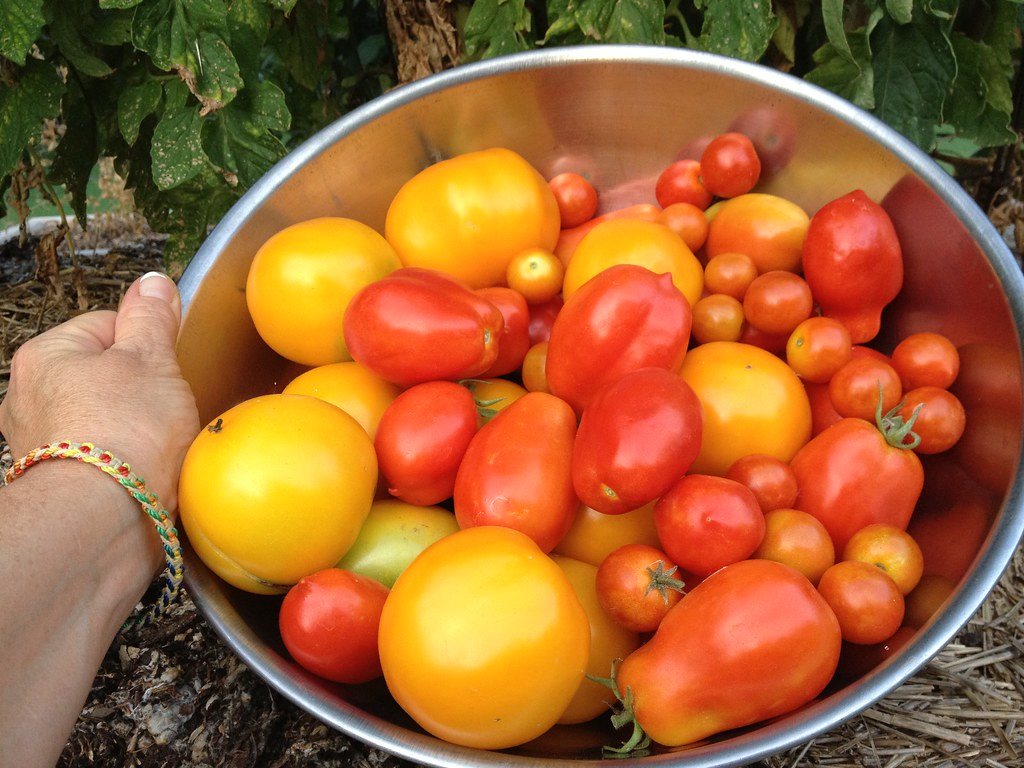
\includegraphics[width=3.91667in,height=\textheight]{images/TomatoHarvest.jpg}

\caption{\label{fig-tomatoes}``\href{https://www.flickr.com/photos/47264866@N00/9455141053}{Tomato
Harvest, Yellow \& Red}'' by
\href{https://www.flickr.com/photos/47264866@N00}{OakleyOriginals} is
licensed under
\href{https://creativecommons.org/licenses/by/2.0/?ref=openverse}{CC BY
2.0}.}

\end{figure}%
\end{quote}

Last but not least, in choosing to learn \texttt{R}, you are entering a
vibrant community of users. As an open-source programming environment,
\texttt{R} is the product of many different people's contributions.
Everyday, new packages, functions, and resources are being developed,
improved, and shared with the community. Given that \texttt{R} has
evolved into one of the most popular languages for scientific
programming (and has become ``the de facto standard in the language
sciences'' Winter 2019: xiii), many of these have been created by
scientists and are particularly well-suited to research workflows.
Moreover, the \texttt{R} community is known for being welcoming,
supportive, and inclusive (sadly, the same cannot be said of all
communities in the computing world). This is reflected in the strong
presence of many community-led initiatives such as
\href{https://rladies.org/}{RLadies} and
\href{https://rainbowr.netlify.app/}{RainbowR}, which encourage
under-represented groups to participate in and contribute to the
\texttt{R} community. 🤗

\begin{figure}

\centering{


\includegraphics[width=2.60417in,height=\textheight]{images/rladiesrp_logo.png}

}

\caption{\label{fig-RLadies}Logo of the
\href{https://rladiesrp.github.io/}{RLadies Ribeirão Preto} meet-up
group, one of
\href{https://benubah.github.io/r-community-explorer/rladies.html}{many
RLadies chapters}.}

\end{figure}%

\subsection*{\texorpdfstring{\emph{``Look, I am studying languages so
why should I learn to code?''}
🤔}{``Look, I am studying languages so why should I learn to code?'' 🤔}}\label{look-i-am-studying-languages-so-why-should-i-learn-to-code}
\addcontentsline{toc}{subsection}{\emph{``Look, I am studying languages
so why should I learn to code?''} 🤔}

Using scripts rather than GUI software will help you make your research
less error-prone, more transparent, and sustainable. Being open-source,
there are no restrictions as to who can run \texttt{R} code and older
versions are available ensuring that exact reproduction is possible,
even years later. As many other language scientists use \texttt{R}, you
will be able to collaborate with others and understand other
researchers' \texttt{R} code. As we will see in a future chapter, in
\texttt{RStudio}, it is also very easy to export \texttt{R} code and
share your scripts, for example as part of an appendix to your research
publication, in various formats (including \texttt{.html} that can be
opened in any browser and \texttt{.pdf}).

In addition, learning to code in \texttt{R} is an excellent way to
understand the basics of data literacy and statistical reasoning. These
are skills that are highly valued among employers, both in academia and
the industry. Many companies, public institutions (e.g., ministries,
hospitals, national agencies) and NGOs hire data scientists who often
work in \texttt{R}. And, even if you end up doing little to no coding
yourself, understanding the basic principles of programming is
undoubtedly a highly useful skill in the modern world.

\begin{tcolorbox}[enhanced jigsaw, breakable, colbacktitle=quarto-callout-note-color!10!white, bottomtitle=1mm, colframe=quarto-callout-note-color-frame, leftrule=.75mm, bottomrule=.15mm, colback=white, toptitle=1mm, rightrule=.15mm, title=\textcolor{quarto-callout-note-color}{\faInfo}\hspace{0.5em}{What about learning Python instead?}, coltitle=black, opacityback=0, arc=.35mm, left=2mm, titlerule=0mm, toprule=.15mm, opacitybacktitle=0.6]

Some of you may be wondering whether you should be learning
\texttt{Python} rather than \texttt{R}. Both are widely used languages
in scientific programming and data science. At the time of writing,
there are more resources specifically aimed at linguists and education
researchers in \texttt{R} than there are in Python simply because it is
currently the most widely used language in these disciplines. Should you
wish to learn \texttt{Python} at a later stage, many of the same
principles that you will have learned in this textbook will apply: it
should feel somewhat like learning Italian when you already speak
Spanish or French.

\end{tcolorbox}

\section{Installing R and RStudio}\label{installing-r-and-rstudio-1}

\subsection{\texorpdfstring{What are \texttt{R} and \texttt{RStudio}?
And why do I need
both?}{What are R and RStudio? And why do I need both?}}\label{what-are-r-and-rstudio-and-why-do-i-need-both}

As a beginner, it's easy to confuse \texttt{R} and \texttt{RStudio}, but
it's important to understand that they are two very different things.
\texttt{R} is a programming environment for statistical computing and
graphics that uses the programming language \texttt{R}. Think of it as
the engine with which we will learn to perform lots of different tasks.
\texttt{RStudio}, by contrast, is a set of tools, a so-called
`integrated development environment' (IDE). It makes working in
\texttt{R} much more intuitive and efficient. If \texttt{R} is the
engine of our car, you can imagine \texttt{RStudio} as our dashboard.
Hence, even though we will later on appear to only be working in
\texttt{RStudio}, \texttt{R} will actually be doing the heavy-lifting,
under the hood.

\begin{figure}

\begin{minipage}{0.50\linewidth}

\centering{


\includegraphics[width=2.40625in,height=\textheight]{images/Rlogo.png}

}

\subcaption{\label{fig-RLogo}Logo of the programming language and
environment \texttt{R}}

\end{minipage}%
%
\begin{minipage}{0.50\linewidth}

\centering{


\includegraphics[width=1.92708in,height=1.85417in]{images/RStudio-Logo_Trademark.png}

}

\subcaption{\label{fig-RStudioLogo}Logo of the IDE \texttt{RStudio}
(RStudio® is a trademark of Posit Software, PBC)}

\end{minipage}%

\caption{\label{fig-Logos}Even the two logos are easy to confuse, but
remember that \texttt{R} and \texttt{RStudio} are two very different
things!}

\end{figure}%

\begin{tcolorbox}[enhanced jigsaw, breakable, colbacktitle=quarto-callout-note-color!10!white, bottomtitle=1mm, colframe=quarto-callout-note-color-frame, leftrule=.75mm, bottomrule=.15mm, colback=white, toptitle=1mm, rightrule=.15mm, title=\textcolor{quarto-callout-note-color}{\faInfo}\hspace{0.5em}{Using other IDEs to work in \texttt{R}}, coltitle=black, opacityback=0, arc=.35mm, left=2mm, titlerule=0mm, toprule=.15mm, opacitybacktitle=0.6]

At the time of writing, \texttt{RStudio} is the most widely used
Integrated Development Environment (IDE) to work in \texttt{R}. However,
it is worth noting that many other IDEs that can be used to access
\texttt{R}. These include:

\begin{itemize}
\item
  \href{https://jupyter.org/}{Jupyter notebook}
\item
  \href{https://code.visualstudio.com/}{Visual Studio Code}
\item
  \href{https://www.jetbrains.com/pycharm/}{PyCharm}
\item
  \href{https://eclipseide.org/}{Eclipse}
\end{itemize}

Whilst this textbook will assume that everyone is working in
\texttt{RStudio}, if you are already familiar with another IDE that
works well with \texttt{R}, you are welcome to continue working in that
IDE. Each IDE has a different feel to it and offers different functions
so, ultimately, it'll be up to you to find the one that suits you best!

\end{tcolorbox}

\subsection{\texorpdfstring{Installing
\texttt{R}}{Installing R}}\label{installing-r}

\begin{enumerate}
\def\labelenumi{\arabic{enumi}.}
\item
  Go to the website of the Comprehensive R Archive Network (CRAN):
  \url{https://cran.r-project.org}.
\item
  Click on the ``Download R for \ldots{}'' link that matches your
  operating system (Linux, macOS or Windows), then:

  \begin{itemize}
  \tightlist
  \item
    For Windows, click on the top `base' link, also marked as ``install
    R for the first time'' (Note that you should also use this link if
    you are updating your R version). On the next page, click on the top
    ``Download R'' link.
  \item
    For MacOS, click on either the top \texttt{.pkg} link if you have an
    Apple silicon Mac (e.g., M1, M2, M3) or the second \texttt{.pkg}
    link, if you have an older Intel Mac.
  \item
    For Linux, click on your Linux distribution and then follow the
    instructions on the following pages.
  \end{itemize}
\end{enumerate}

\begin{enumerate}
\def\labelenumi{\arabic{enumi}.}
\setcounter{enumi}{2}
\item
  Once you have downloaded one of these \texttt{R} versions, navigate to
  the folder where you have saved it (by default, this will be your
  Downloads folder), and double click on the executable file to install
  \texttt{R}.
\item
  Follow the on-screen instructions to install \texttt{R}.
\item
  Test that \texttt{R} is correctly installed. On Windows and MacOS,
  navigate to your Applications folder and double click on the
  \texttt{R} icon. On Linux, open up \texttt{R} by typing \texttt{R} in
  your terminal. This should open up an R Console. You can type R
  commands into the Console after the command prompt
  \texttt{\textgreater{}}. Type the following R code after the command
  prompt and then press enter: \texttt{plot(1:10)}.
\end{enumerate}

\begin{figure}

\begin{minipage}{0.50\linewidth}

\centering{

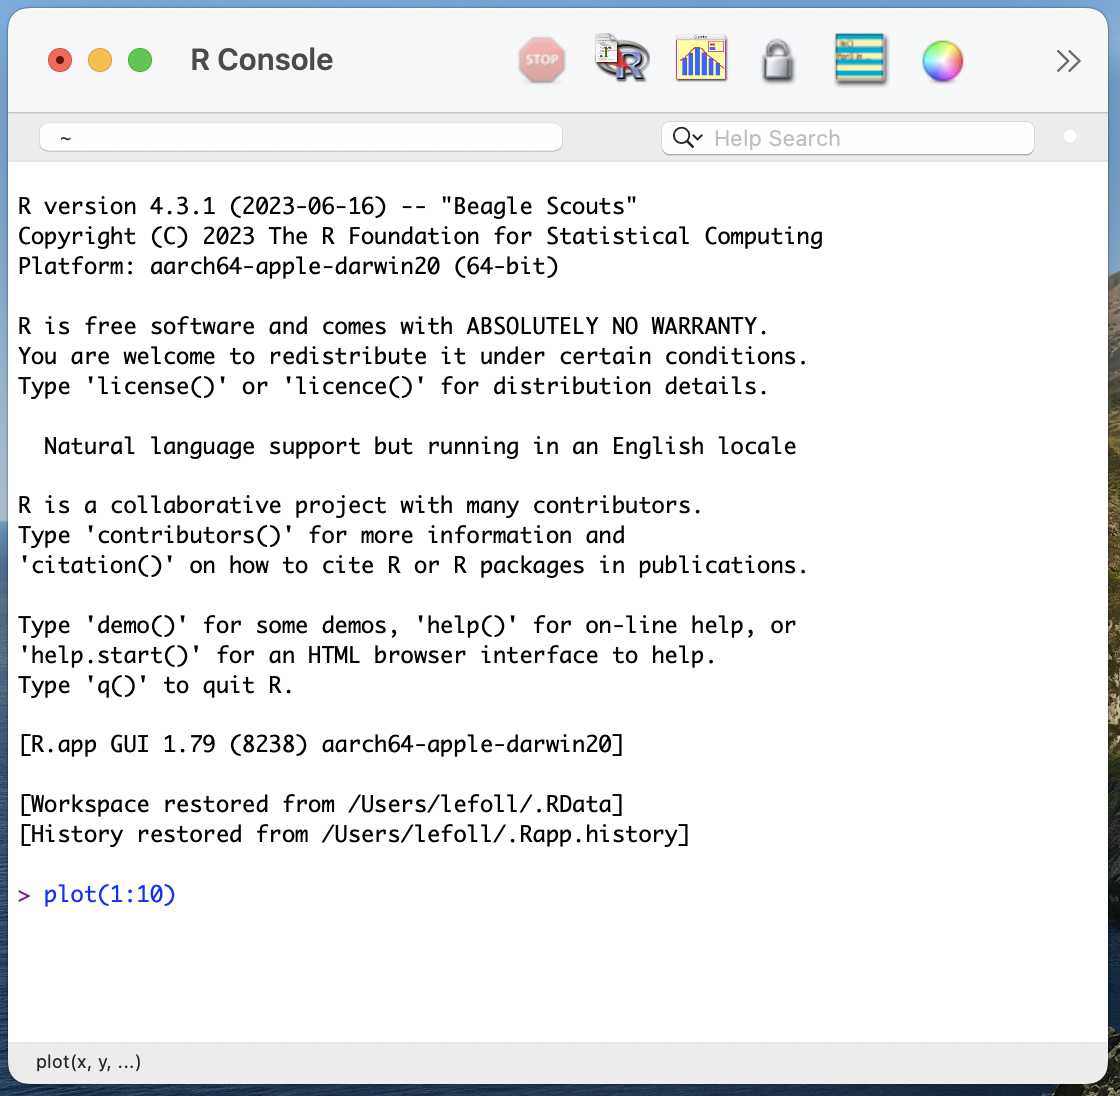
\includegraphics{images/RConsole.png}

}

\subcaption{\label{fig-console}Test command in the R Console}

\end{minipage}%
%
\begin{minipage}{0.50\linewidth}

\centering{

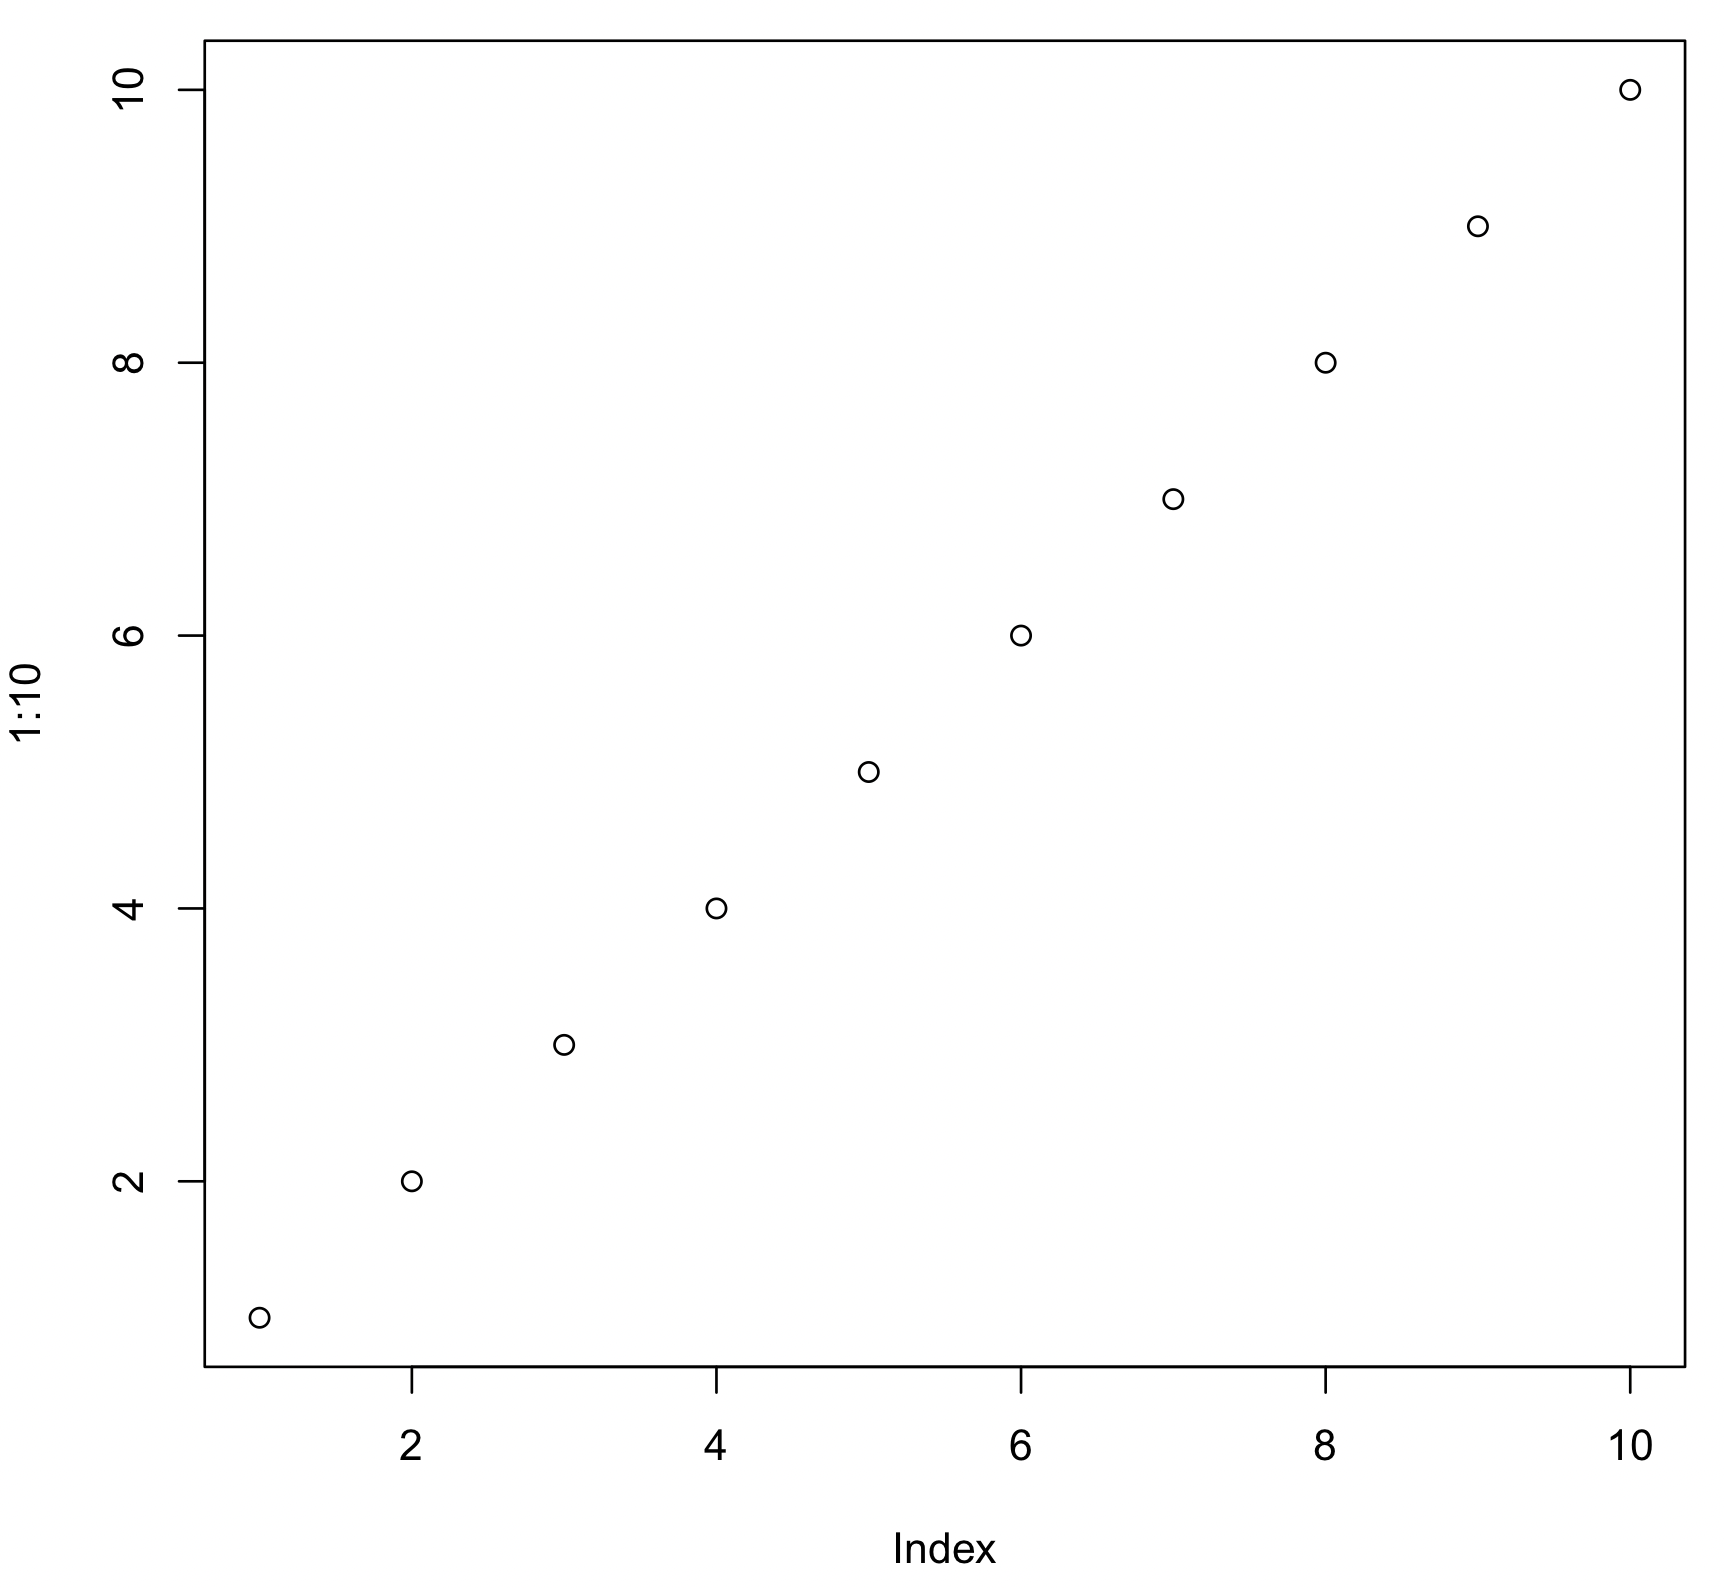
\includegraphics{images/TestingRPlot.png}

}

\subcaption{\label{fig-testplot}Resulting plot (note that the
proportions of your plot may be different depending on the size of your
window)}

\end{minipage}%

\caption{\label{fig-Rtest}Testing R}

\end{figure}%

✅ If you see the plot above, you have successfully installed and tested
\texttt{R} and you can go on to installing \texttt{RStudio}.

⚠️ If that's not the case, make a note of the errors produced (copy and
paste them into a text document or take a screenshot) and search for
solutions on the Internet. It is very likely that many other people have
already encountered the same problem as you and that someone from the
\texttt{R} community has posted a solution online.

\begin{tcolorbox}[enhanced jigsaw, breakable, colbacktitle=quarto-callout-note-color!10!white, bottomtitle=1mm, colframe=quarto-callout-note-color-frame, leftrule=.75mm, bottomrule=.15mm, colback=white, toptitle=1mm, rightrule=.15mm, title=\textcolor{quarto-callout-note-color}{\faInfo}\hspace{0.5em}{What to do if you cannot get R and/or RStudio working on your computer}, coltitle=black, opacityback=0, arc=.35mm, left=2mm, titlerule=0mm, toprule=.15mm, opacitybacktitle=0.6]

The aim of this chapter is to install both \texttt{R} and
\texttt{R\ Studio} on your own computer so that you can write and run
your own scripts locally (i.e., on your own computer without the need
for an internet connection). In some cases, however, this might not be
possible. For example, because the programmes are not available for your
operating system, or because you do not have admin rights on your
computer, or because your disk is full and you cannot delete anything.
None of these situations are ideal to do research, but don't give up on
learning \texttt{R}: there is an alternative!

You can sign up to \href{https://posit.co/products/cloud/cloud/}{Posit
Cloud}. Posit Cloud will allow you to run \texttt{R} in \texttt{RStudio}
in a browser (e.g., Firefox or Chrome) without having to install
anything on your computer. Although Posit Cloud's
\href{https://posit.cloud/plans/free}{free plan} is limited, it will
suffice to learn the contents of this textbook. You will be able to
follow the textbook in exactly the same way as everyone else. However,
you will need a stable internet connection and you may find that you
need to be a bit more patient as things are likely to run a little
slower. If you decide to opt for the Posit Cloud solution, create a free
account and then go straight to Setting up RStudio.

\end{tcolorbox}

\subsection{\texorpdfstring{Installing
\texttt{RStudio}}{Installing RStudio}}\label{installing-rstudio}

When you head over to their website, it may be confusing to you that the
company that provides \texttt{RStudio}, Posit, also offers paid-for
versions of \texttt{RStudio} and other paying services. Do not worry, we
will not need any of these: These are products designed for companies
and large organisations. The version of \texttt{RStudio\ Desktop} that
we will be using, however, is completely free and, given that it is open
source, even if Posit decided to stop working on this product one day,
others in the \texttt{R} community would take over. Such is the beauty
of
\href{https://elenlefoll.github.io/RstatsTextbook/OpenScholarship.html}{open-source
software}! 🤗

\begin{enumerate}
\def\labelenumi{\arabic{enumi}.}
\item
  Head over to this page
  \url{https://posit.co/download/rstudio-desktop/} to download the
  latest version of \texttt{RStudio\ Desktop}.
\item
  As you have already installed \texttt{R}, you can jump straight to
  step ``2: Install RStudio''. The website should have detected which
  operating system your computer is running on, so that you can most
  likely simply click on the ``Download RStudio Desktop\ldots{}''
  button. Your download should start straight away.

  \begin{itemize}
  \tightlist
  \item
    If an incorrect operating system is detected, simply scroll down the
    page to find your operating system and download the corresponding
    version of \texttt{RStudio.}
  \end{itemize}
\end{enumerate}

\begin{enumerate}
\def\labelenumi{\arabic{enumi}.}
\setcounter{enumi}{2}
\item
  Once you have downloaded \texttt{RStudio}, navigate to the folder
  where the downloaded file has been saved (by default, this will be
  your Downloads folder), and double click on the executable file to
  install \texttt{RStudio}.
\item
  Follow the on-screen instructions to install \texttt{RStudio}.
\end{enumerate}

If you run into any issues that you cannot solve with existing online
posts, the \href{https://forum.posit.co/}{Posit Community forums} are a
good place to ask for help.

\section{Setting up RStudio}\label{setting-up-rstudio}

From now on, we will only be accessing \texttt{R} through
\texttt{RStudio}. When you open up \texttt{RStudio} for the first time,
you might find the layout rather intimidating. The application window is
divided into several sections, which we call `panes'. Each pane also has
several tabs. Although it may seem overwhelming at first, you will soon
see that these different panes and tabs will actually make life much
easier.

\subsection{Global options}\label{global-options}

Before we get staRted properly, however, we need to change some of the
default settings of \texttt{RStudio}. The first set of changes that we
are going to make ensure that, each time we launch a new \texttt{R}
session in \texttt{RStudio}, we are starting afresh.

To do so, head over to the `Tools' dropdown menu and click on `Global
Options'. Make sure that the first three boxes are unticked (see
Figure~\ref{fig-GOGeneral}). Under ``Save workspace to .RData on exit'',
select the option ``Never''. Always starting afresh is good programming
practice. It avoids any problems being carried over from previous
\texttt{R} sessions. You can think of it like cooking in a freshly
cleaned, tidy kitchen. It's much safer than preparing a meal in a messy,
possibly even contaminated kitchen! {\marginnote{\begin{footnotesize}Or
use the keyboard shortcut
\texttt{Ctrl/Command\ +\ ,}\end{footnotesize}}}

\begin{figure}

\begin{minipage}{0.50\linewidth}

\centering{

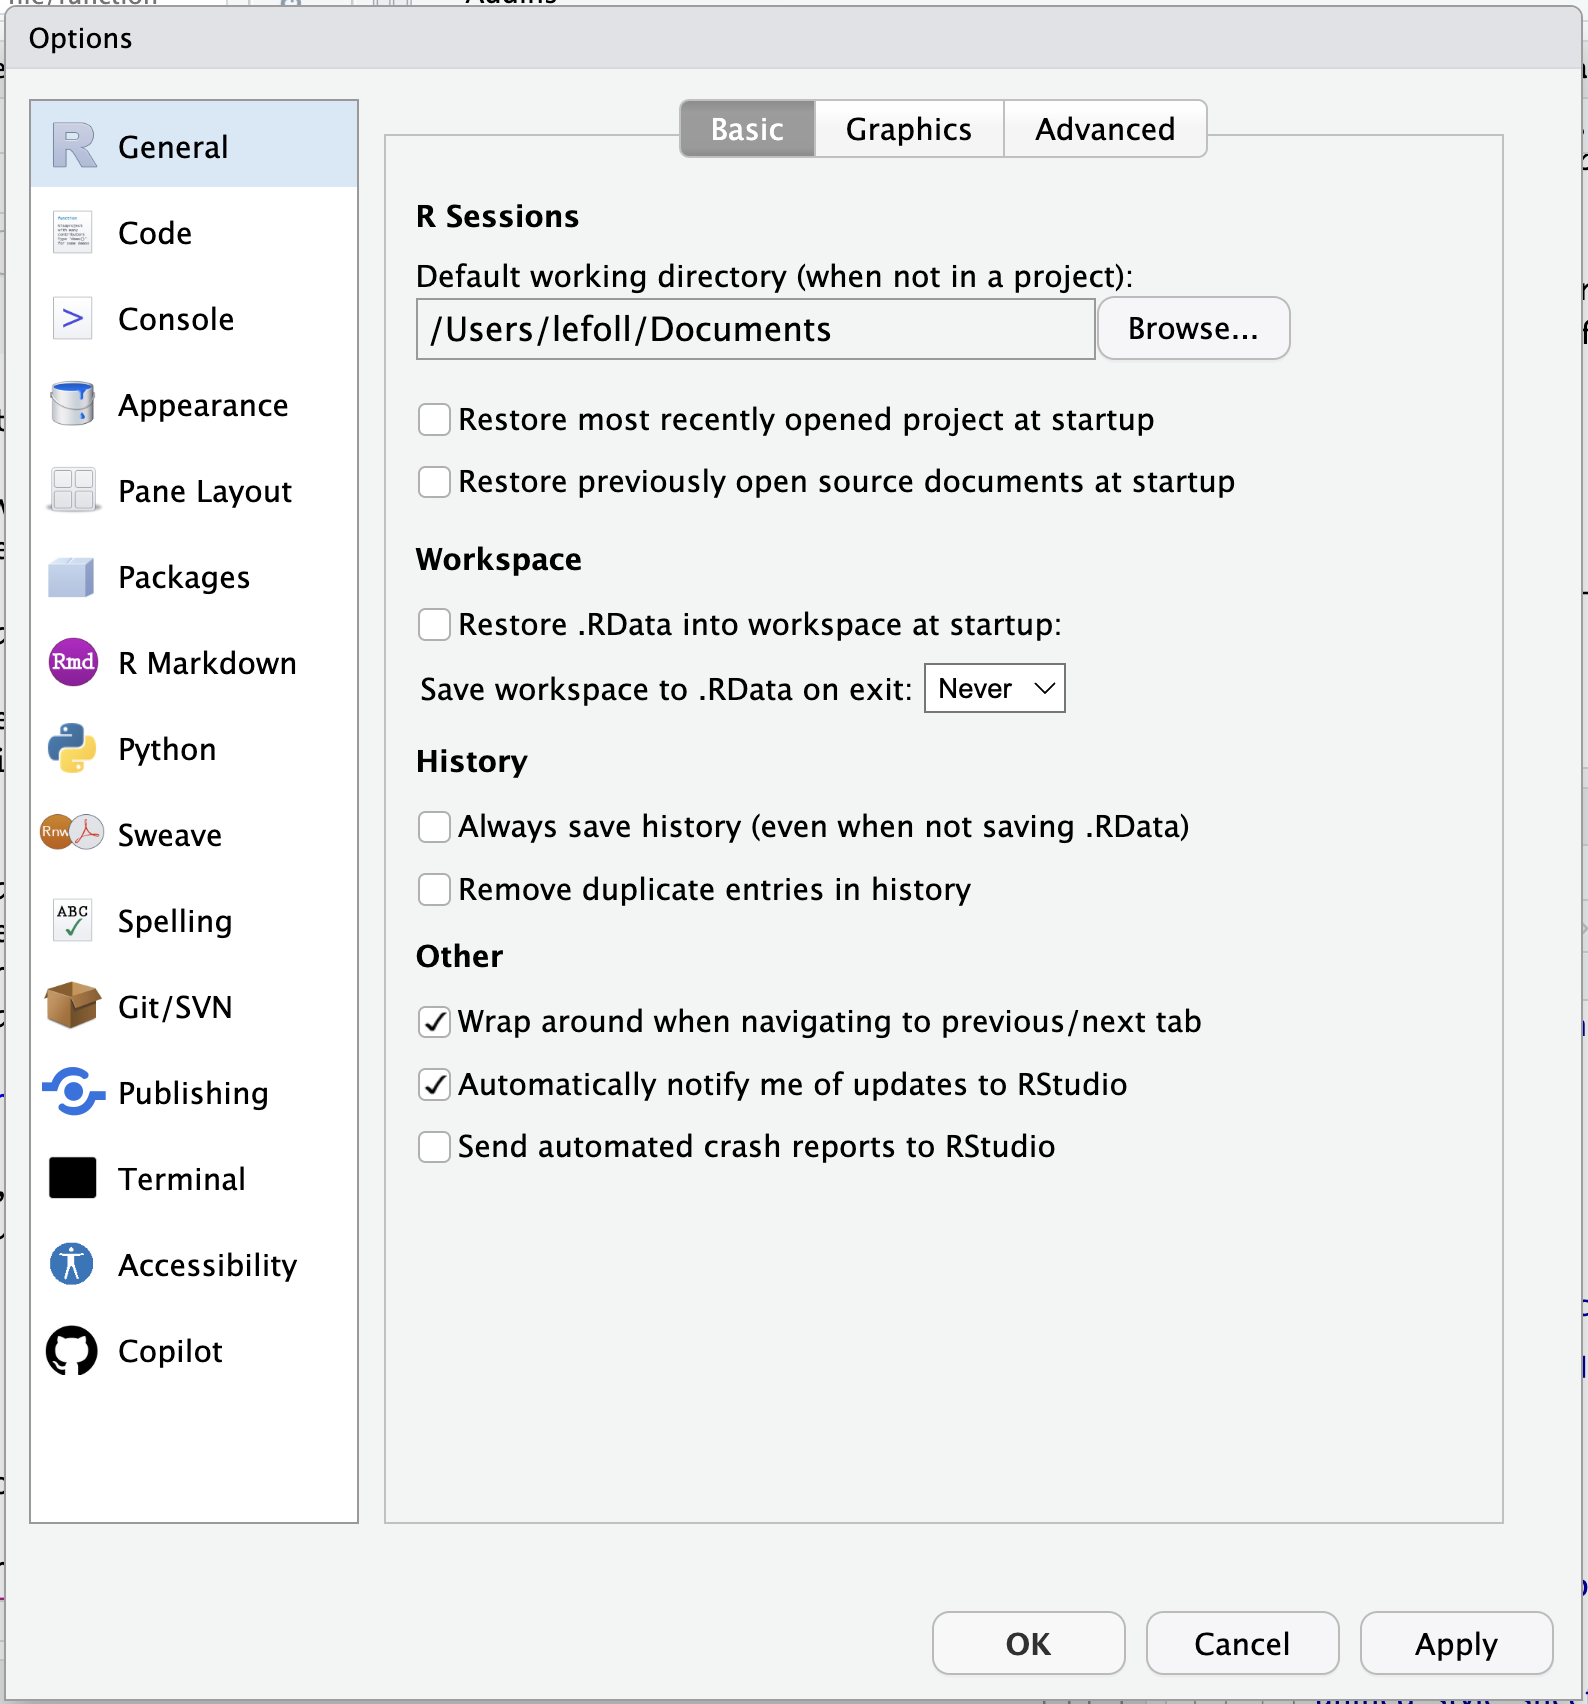
\includegraphics{images/RStudioGlobalOptionsGeneral.png}

}

\subcaption{\label{fig-GOGeneral}General tab}

\end{minipage}%
%
\begin{minipage}{0.50\linewidth}

\centering{

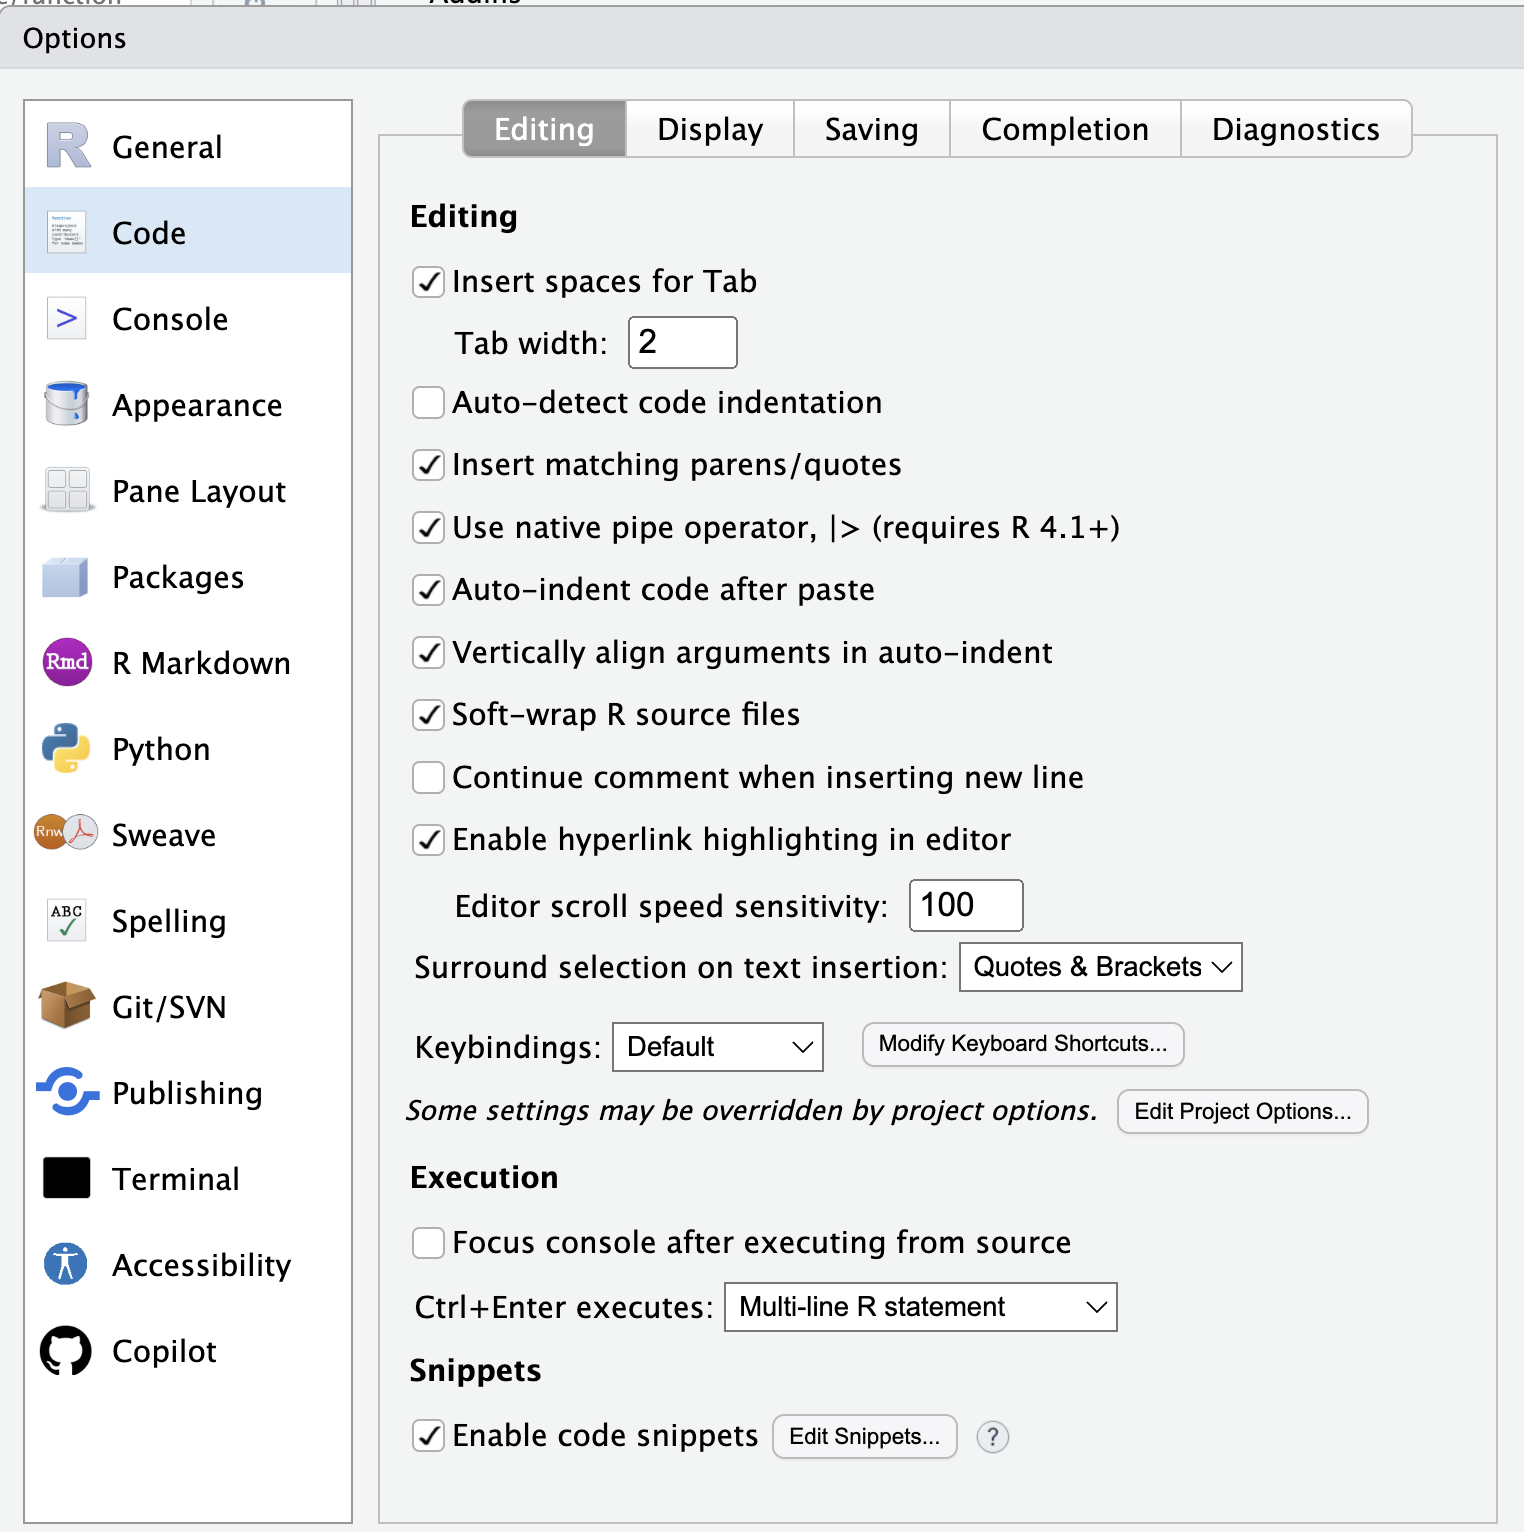
\includegraphics{images/RStudioGlobalOptionsCode.png}

}

\subcaption{\label{fig-GOCode}Code tab}

\end{minipage}%

\caption{\label{fig-GlobalOptions}RStudio's Global Options}

\end{figure}%

Next, under the `Global Options' tab `Code' of the `Global Options'
window, ensure that the option ``Use native pipe operator'' is ticked
(see Figure~\ref{fig-GOCode}). This is a new feature in \texttt{R} that
is very useful so we will make use of it in this textbook. The other
options are not relevant for now.

Finally, head over to the `Pane Layout' tab. From here, you can
rearrange the panes of your \texttt{RStudio} window. To do so, click on
the ﹀ symbols to get a dropdown menu corresponding to each pane. You
can also select which tabs you would like to see in each pane. If you
are already familiar with \texttt{RStudio}, feel free to stick to your
favourite set-up. Personally, I use the panes layout below and, if you
are new to \texttt{R}, I recommend that you select this layout, too. You
can always go back to these `Global Options' to change this setup at any
stage. Don't forget to click on `OK' at the bottom of the Global Options
page to save your settings. Then, the panes in your \texttt{RStudio}
window should be ordered as in Figure~\ref{fig-RStudioNewLayout}.

\begin{figure}

\begin{minipage}{0.50\linewidth}

\centering{

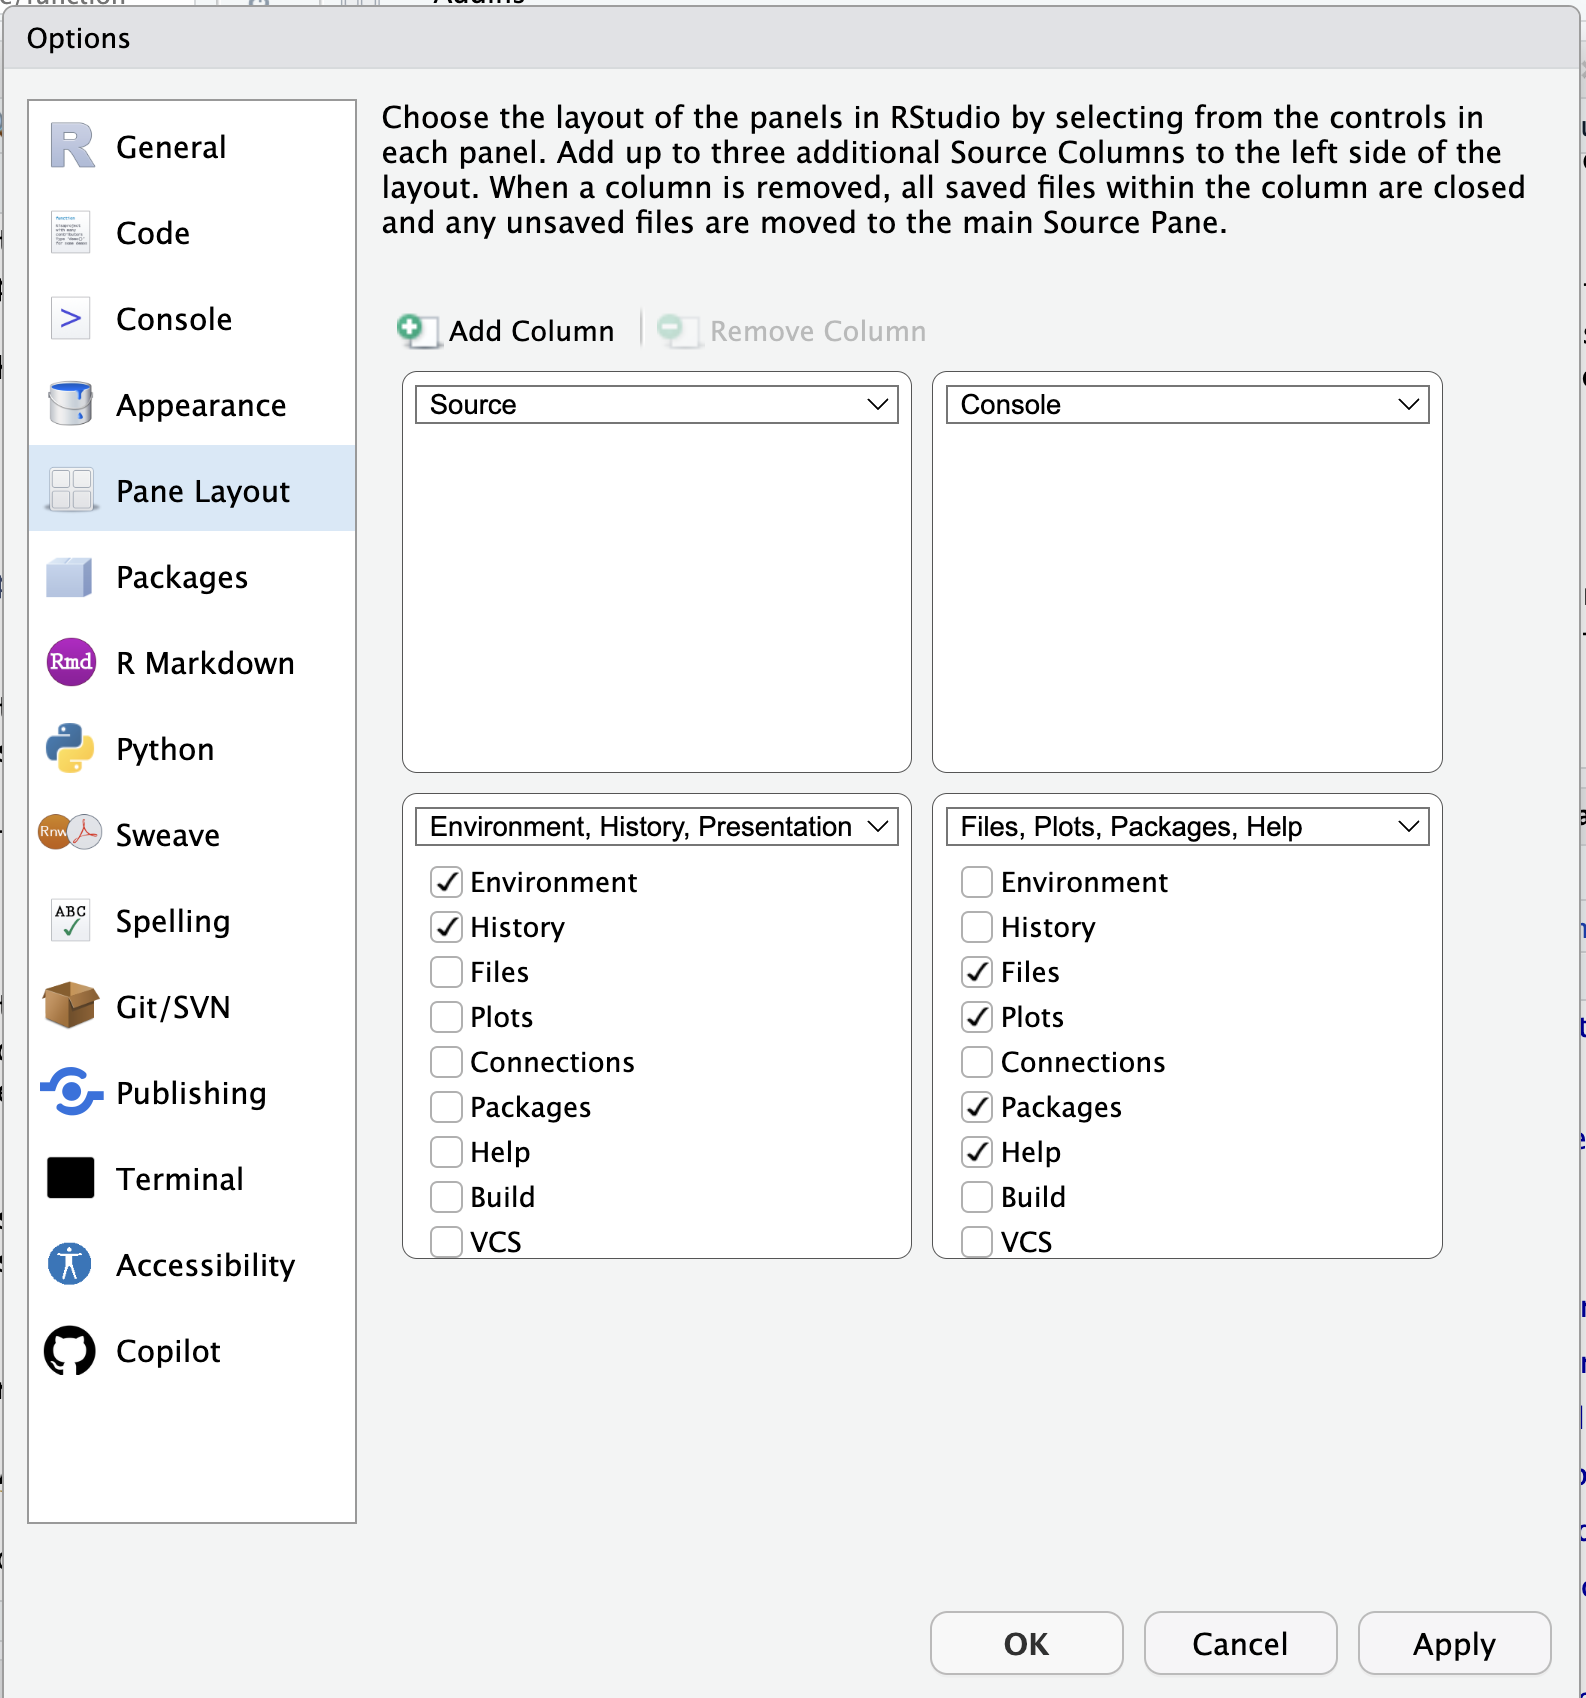
\includegraphics{images/RStudioGlobalOptionsPanes.png}

}

\subcaption{\label{fig-GOPanes}Panes Layout tab}

\end{minipage}%
%
\begin{minipage}{0.50\linewidth}

\centering{

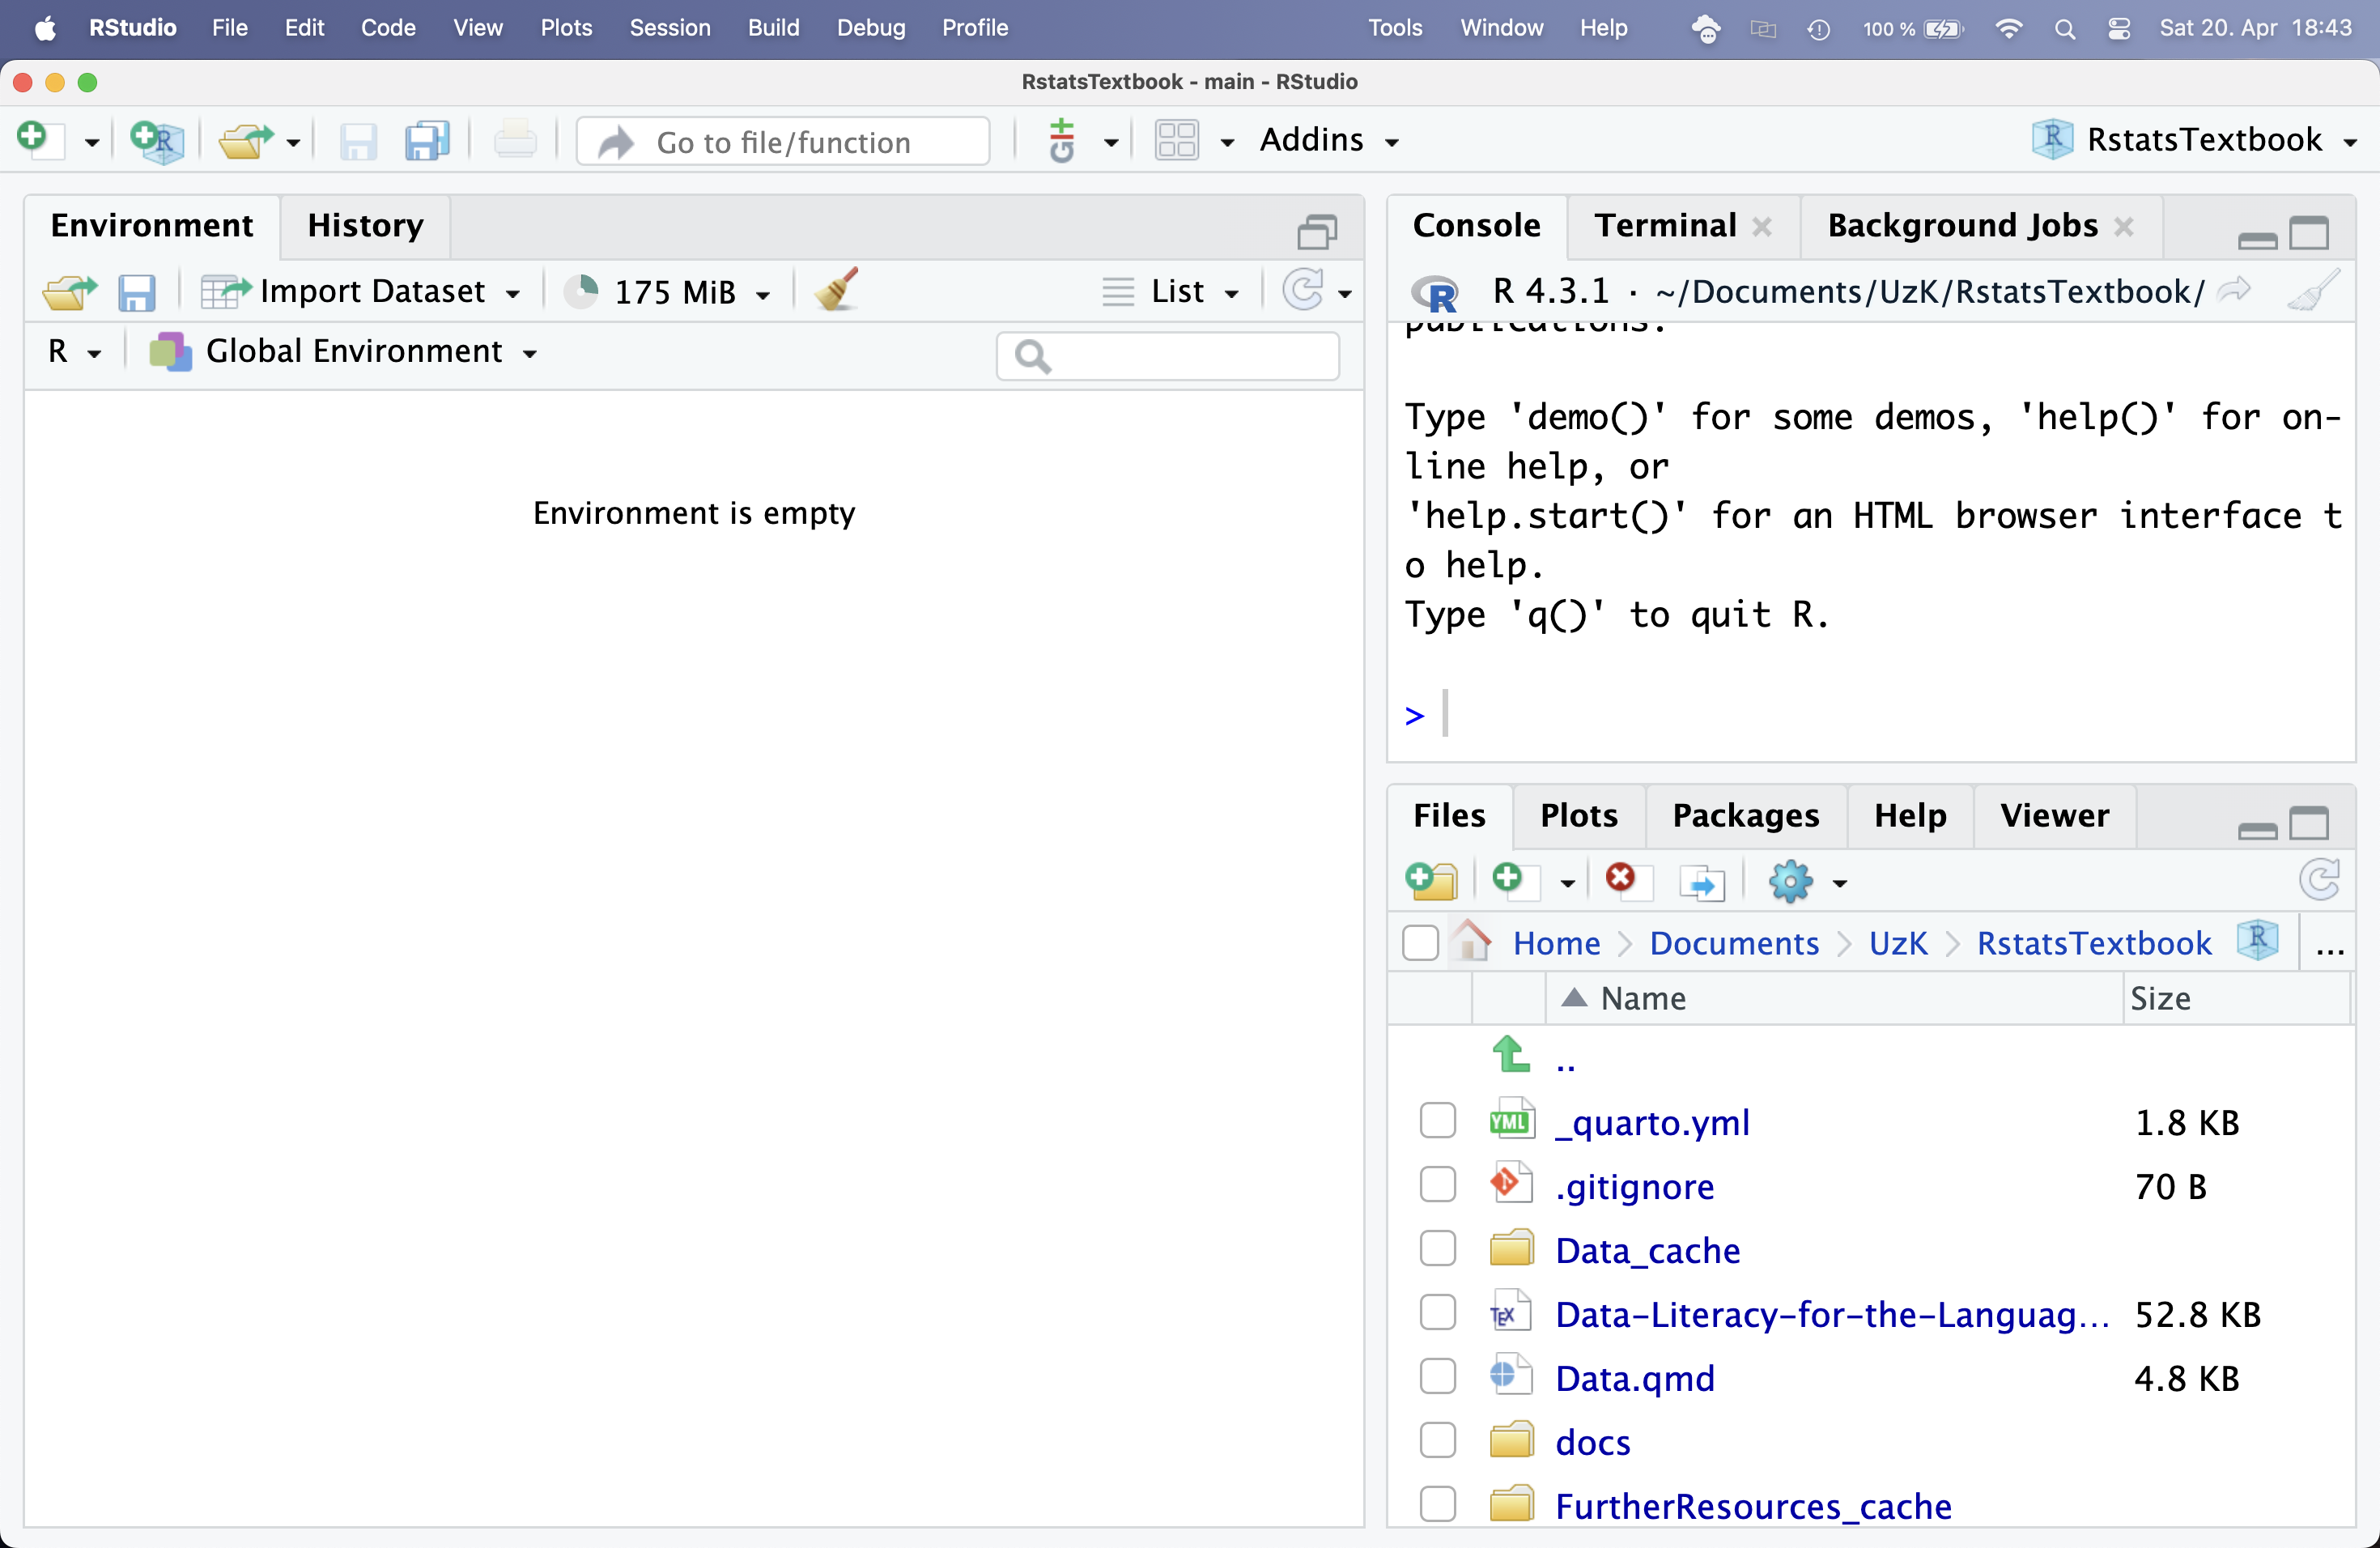
\includegraphics{images/RStudioNewLayout.png}

}

\subcaption{\label{fig-RStudioNewLayout}Customised panes layout}

\end{minipage}%

\caption{\label{fig-Panes}Recommended \texttt{RStudio} panes layout}

\end{figure}%

\subsection{Testing RStudio}\label{testing-rstudio}

It is now time we tested whether \texttt{RStudio} is communicating well
with \texttt{R}. To do so, let's run the same test as in the
\texttt{R\ Console}. This time, head over to the Console tab in the top
right pane of your \texttt{RStudio} window and, after the command prompt
\texttt{\textgreater{}}, type: \texttt{plot(1:10)} and then press enter.
You should see the same plot as earlier on (see
Figure~\ref{fig-testplot}), appearing in the Plots tab of the bottom
right pane of your \texttt{RStudio} window.

If you get the following error message
\texttt{Error\ in\ plot.new()\ :\ figure\ margins\ too\ large}, this is
because your bottom right pane is hidden from view or too small for the
plot to be printed there. Click on the small two-window icon in the
bottom-right corner if it is hidden (see
Figure~\ref{fig-MinimisedPlotPane}). Or, if it too small, click on the
dividing line between the two right-hand side panes and, whilst still
holding down the mouse button, drag up the line until it is about
halfway up. Then, re-type the command \texttt{plot(1:10)} in the Console
pane and press enter again. The plot should appear as in
Figure~\ref{fig-testplotRStudio}.

\begin{figure}

\begin{minipage}{0.50\linewidth}

\centering{

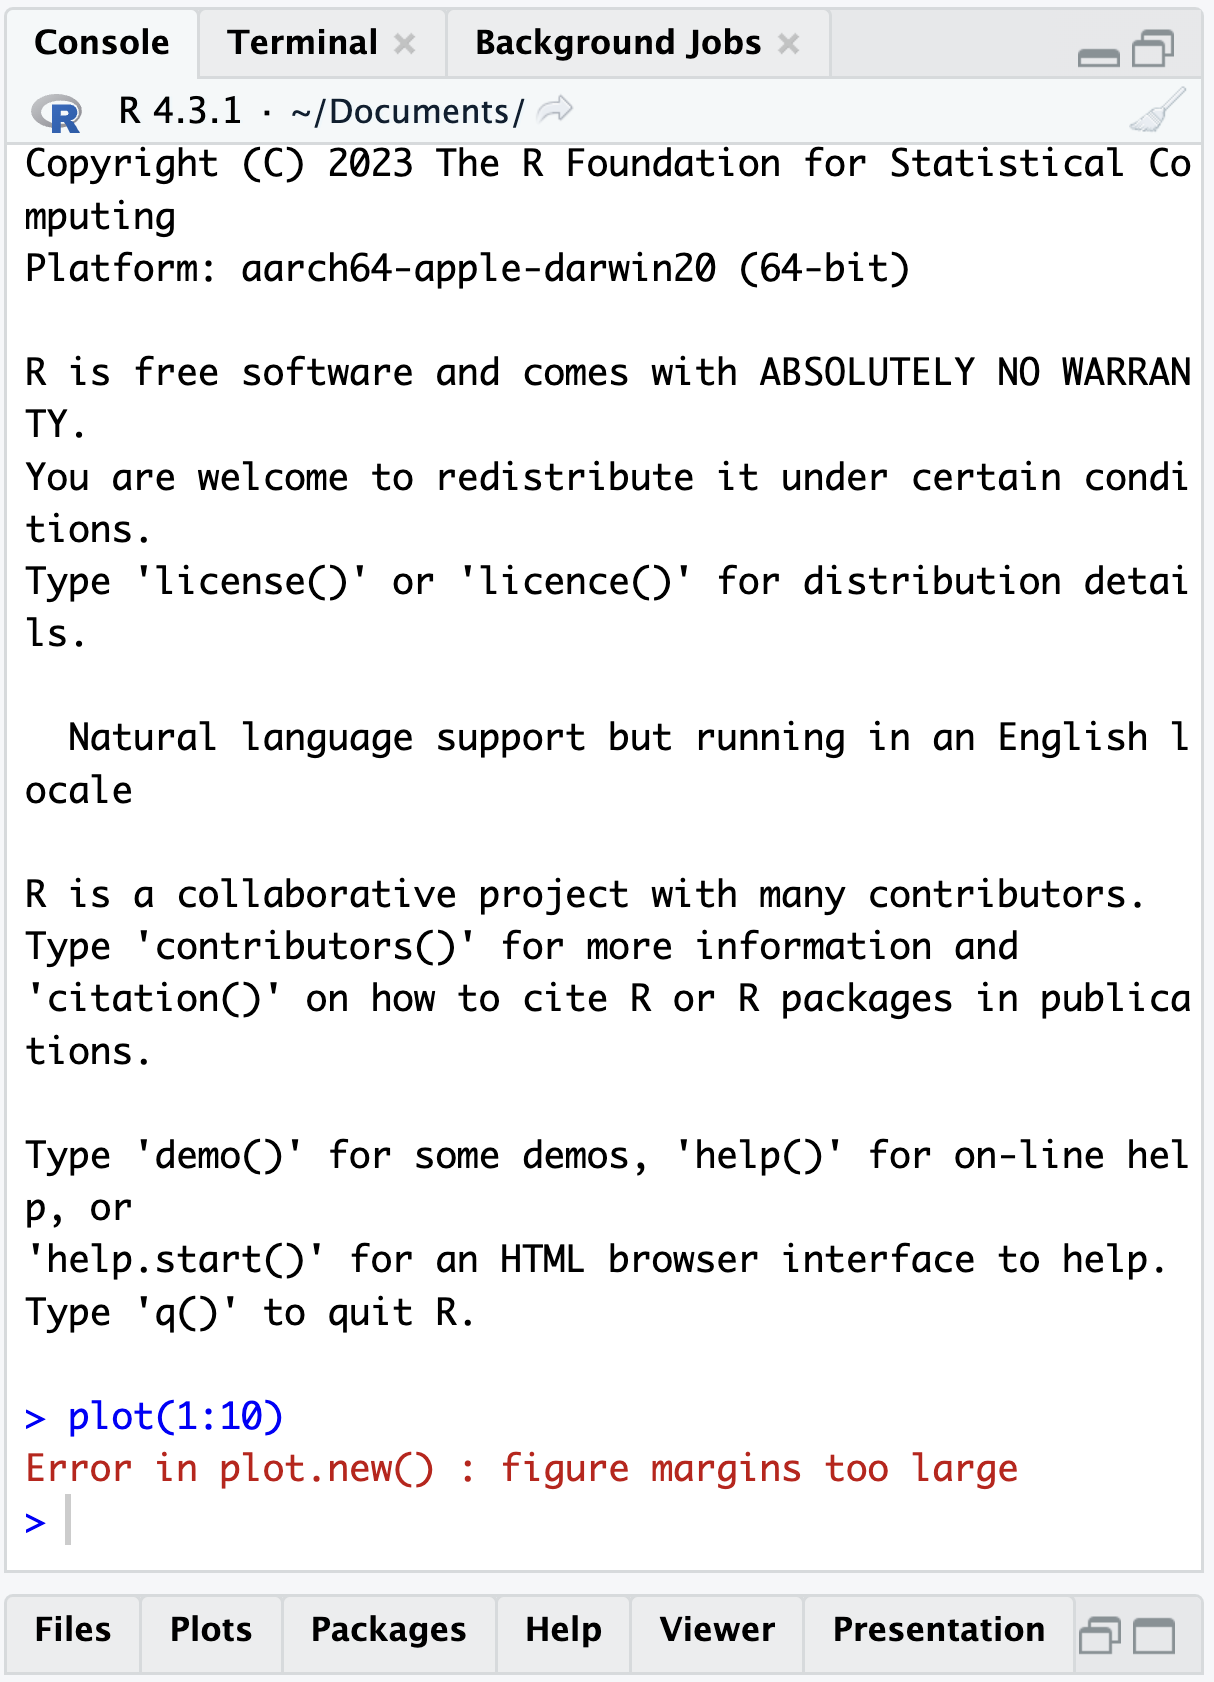
\includegraphics{images/PlotMarginsError.png}

}

\subcaption{\label{fig-MinimisedPlotPane}Hidden (minimised) bottom right
pane}

\end{minipage}%
%
\begin{minipage}{0.50\linewidth}

\centering{

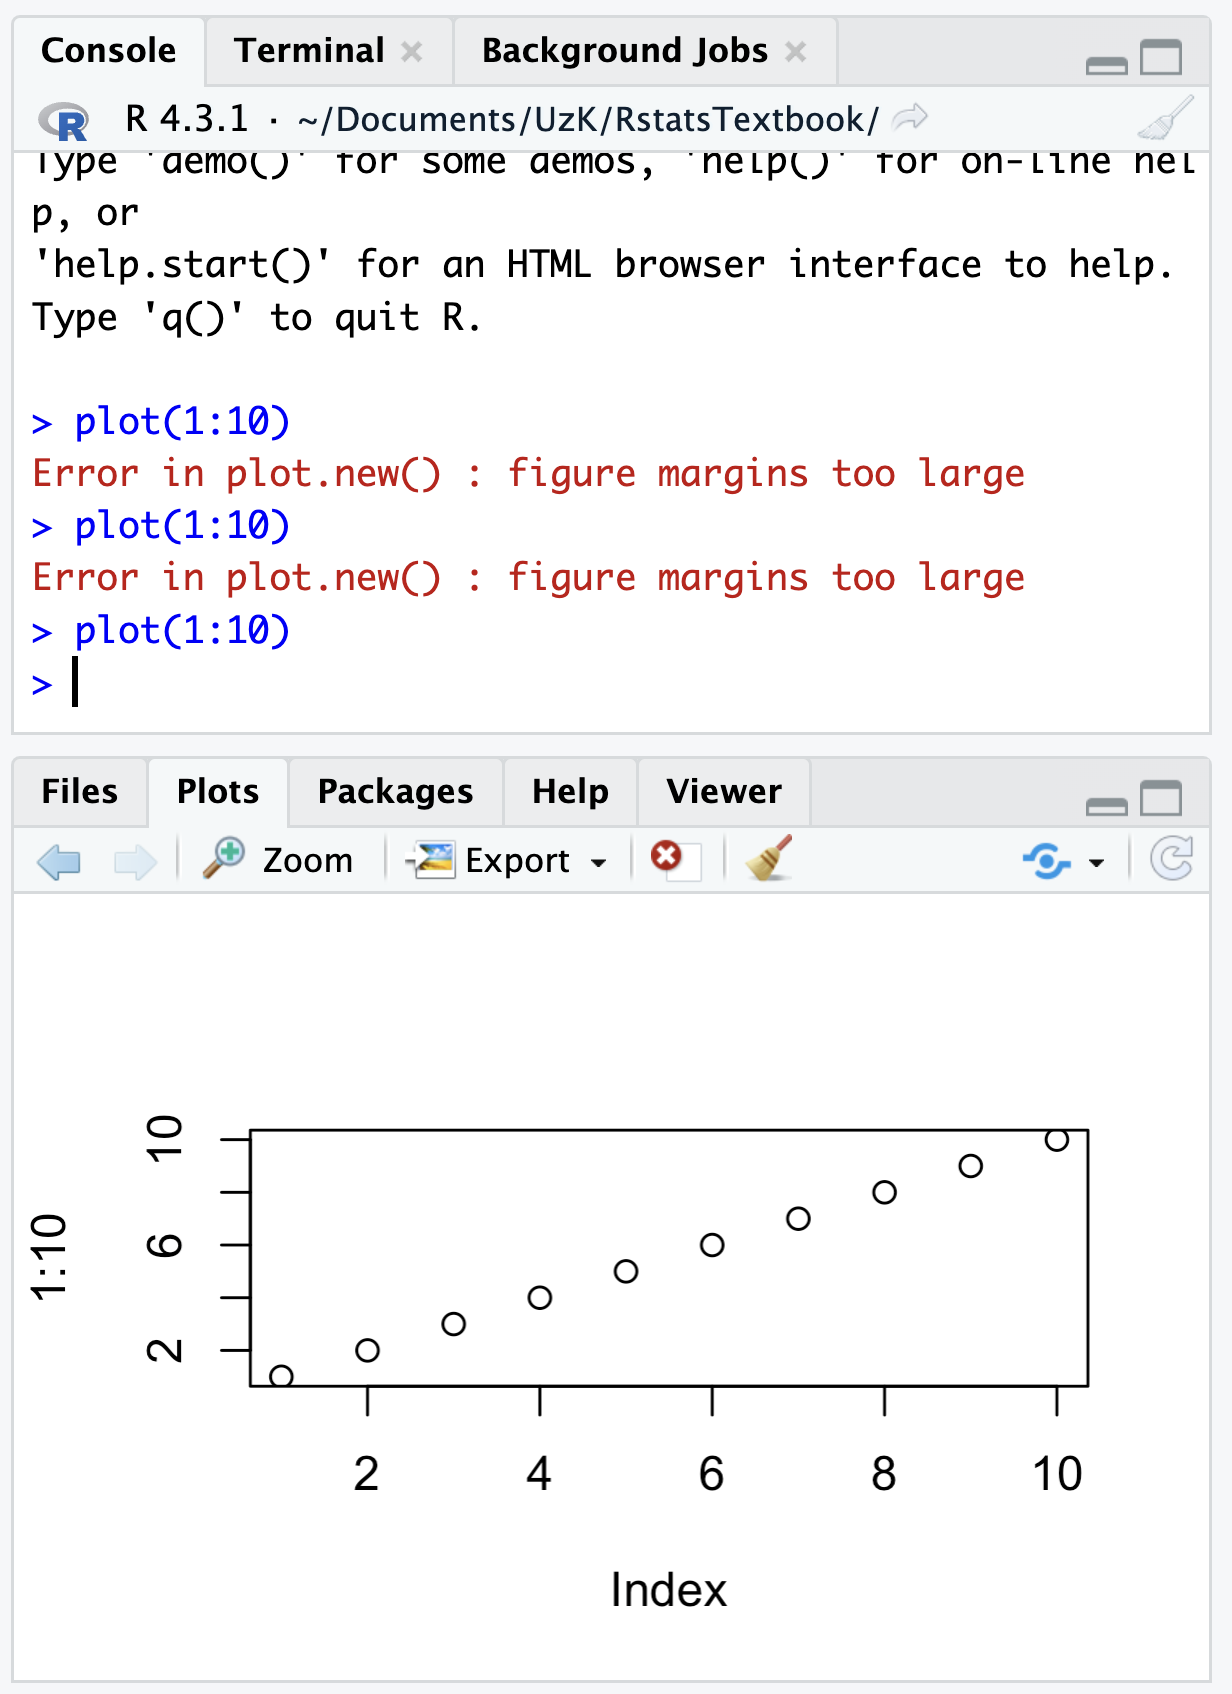
\includegraphics{images/TestplotRStudio.png}

}

\subcaption{\label{fig-testplotRStudio}Now the dividing line between the
two panes is halfway up and the plot has been successfully output in the
Plots pane}

\end{minipage}%

\caption{\label{fig-testingRStudio}Testing that \texttt{RStudio} is
communicating well with your \texttt{R} installation.}

\end{figure}%

\section{\texorpdfstring{Installing \texttt{R}
packages}{Installing R packages}}\label{installing-r-packages}

\subsection{What are packages?}\label{what-are-packages}

You now have a base installation of \texttt{R}. Base \texttt{R} is very
powerful and comes with many standard packages and functions that
\texttt{R} users use on a daily basis. If you click on the Packages tab
in the bottom-right pane and scroll down, you will see that there are
many packages available. Only a few are selected. These are part of the
base \texttt{R} installation.

In addition to the members of the R Core Team who develop and maintain
base \texttt{R}, thousands of \texttt{R} users develop and share
additional \texttt{R} packages every day. These enable us to vastly
increase the capacities of base \texttt{R}. Packages are a very helpful
way to bundle together a set of functions, data, and documentation files
so that other \texttt{R} users can easily download these bundles and add
them to their local \texttt{R} installation.

Throughout this textbook, the names of packages will be enclosed in
curly brackets like this: \{ggplot2\}.

\begin{quote}
\subsubsection*{Quiz time!}\label{quiz-time-1}
\addcontentsline{toc}{subsubsection}{Quiz time!}

1) Which of these packages is not part of base \texttt{R}?

~

2) Is it possible to create an \texttt{R} package that provides access
to the full texts of all of Jane Austen's published novels for
computational text analysis in \texttt{R}?

~

3) Is the \{janeaustenr\} package installed as part of base \texttt{R}?
\end{quote}

\subsection{Installing packages}\label{installing-packages}

To install a package, you will first need to download it from the
internet. Packages are typically stored on different websites (online
repositories), but the most trustworthy one and easiest to work with is
\href{https://cran.rstudio.com/index.html}{CRAN} (Comprehensive R
Archive Network). To install the \{janeaustenr\} package from CRAN,
simply type the following command in the Console pane and then type
enter: \texttt{install.packages("janeaustenr")}.

This command will take a few seconds to run (or longer depending on how
slow your internet connection is). You should then see a message in red
in the console indicating (among other things that you can ignore) that
the package has been successfully downloaded and its size (here: 1.5
megabyte), as well as the path to where the package's content has been
saved on your computer (see Figure~\ref{fig-PckInstalled}). You do not
need to worry about any of the other information.

\begin{figure}

\centering{

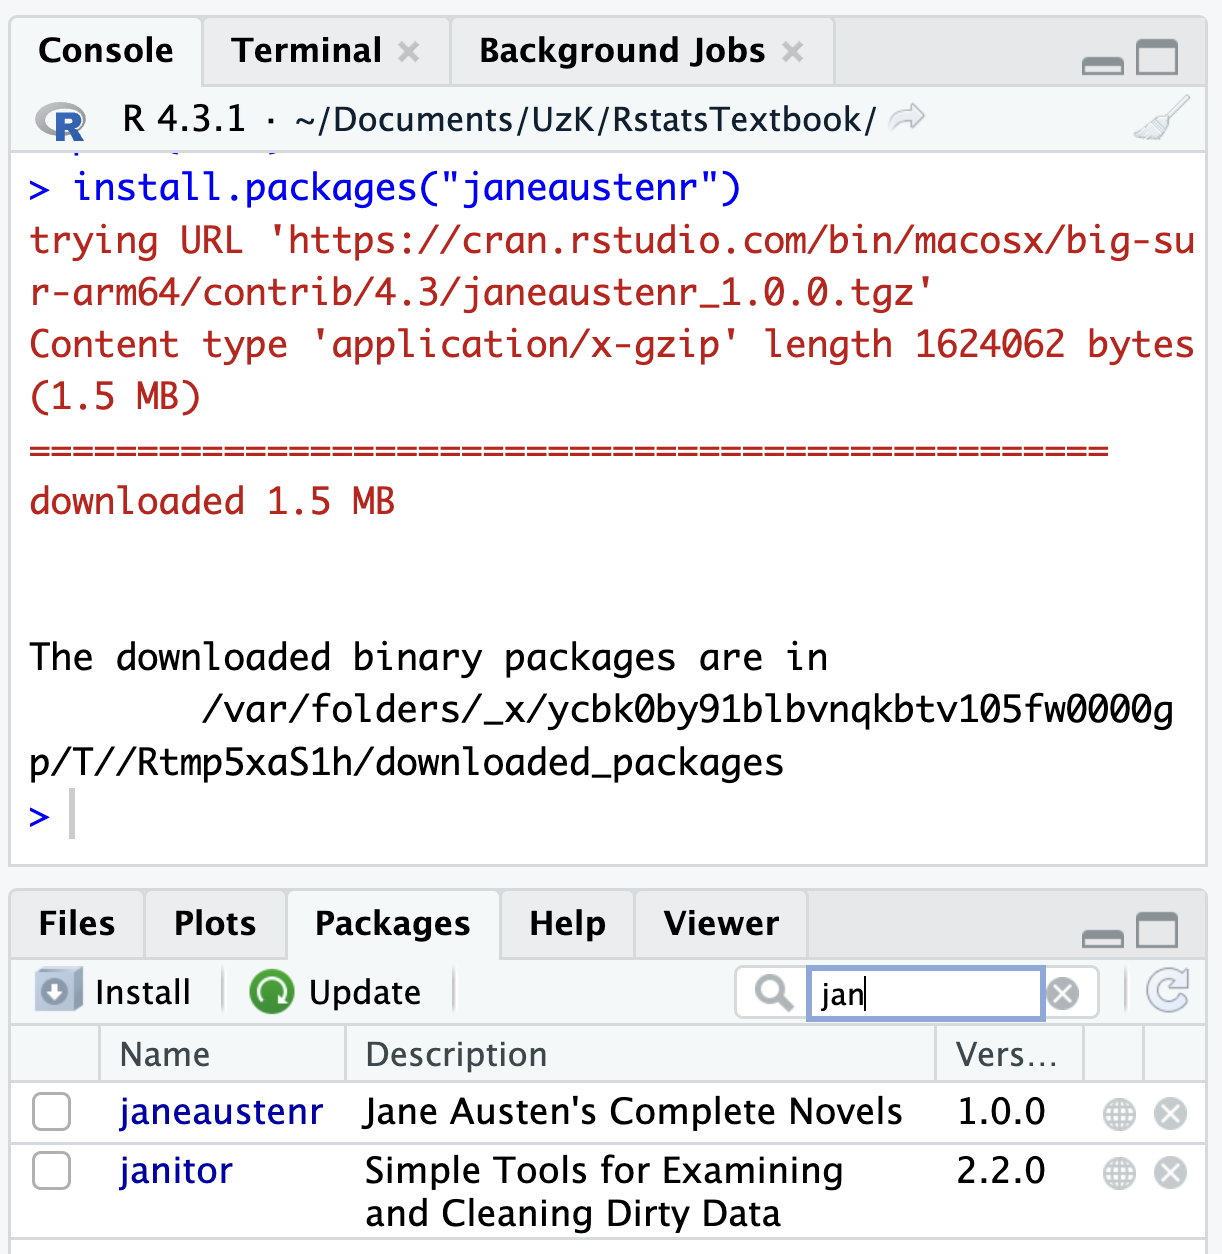
\includegraphics[width=4.6875in,height=\textheight]{images/JaneaustenrInstalled.png}

}

\caption{\label{fig-PckInstalled}Screenshot showing that the package has
been correctly installed.}

\end{figure}%

To check that the package has been successfully downloaded and
installed, head over to the Packages tab of the bottom-right pane and
scroll down to the \{janeaustenr\} package, or search for it using the
search window within this same tab. The \{janeaustenr\} package should
now be visible, which tells us that the package is installed on your
computer. Note, however, that the checkbox next to it is currently
empty. This means that the package hasn't been loaded in our current
\texttt{R} session and therefore cannot be used yet. Note that whilst
you only need to install each package once, you will need to load it
every time we want to use it in a new \texttt{R} session. This is
because, when we start a new \texttt{R} session, the kitchen is
perfectly clean and tidy and everything is back in storage. And the good
news is that we don't even need to do the washing-up! 🙃

\subsection{Loading packages}\label{loading-packages}

You can think of base \texttt{R} as a fully functional student kitchen.
It is rather small and only has the most essential ingredients and
equipment, but it still has everything you need to cook simple,
delicious meals. Downloading and installing additional packages is like
buying fancier ingredients (these are packages that include datasets) or
more sophisticated and specialised kitchen devices (these are packages
that include additional functions).

Once you have downloaded and installed a new package, it is put in
storage (either in the fridge or in a kitchen cupboard). In this case,
the package appears in your Packages tab, but is not yet selected. If
you want to use the new ingredient or the piece of equipment that was
delivered in the new package, you need to get it out of the fridge or
the cupboard and place it on the kitchen counter. This is the equivalent
to loading a package. Once they are unpacked (i.e., installed), packages
are usually referred to as libraries.

So the first thing we now need to do to be able to analyse Jane Austen's
novels in \texttt{R} is to load the \{janeaustenr\} library. The command
to do is \texttt{library(janeaustenr)}. Type this command in the Console
and press enter. Ideally, it should look like nothing has happened.
Indeed, if you do not get an error message (in red), then the library
has been successfully loaded. We can check that this is actually the
case by looking again for the \{janeaustenr\} in the Packages tab. The
checkbox should now be ticked. {\marginnote{\begin{footnotesize}⚠️ Note
that, rather confusingly, both error and warning messages are printed in
red but, for now, we will only worry about error messages. Most warning
messages can safely be ignored.\end{footnotesize}}}

\section{Package documentation}\label{package-documentation}

To find out more about any package or function, simply use the command
\texttt{help()} or its shortcut \texttt{?}. For example, to find out
more about the \{janeaustenr\} package, enter the command
\texttt{help(janeaustenr)} or \texttt{?janeaustenr} in the Console. The
help file will open up in the Help tab of the bottom-right pane. It
contains the name of the package and a short description, as well as the
name of the package maintainer, Julia Silge, and some additional links.

One of these links takes us to the package creator's GitHub repository.
This is where we can find a source code for the package, should we want
to check how it works under the hood, or amend it in any way. Click on
this link and scroll down the package's GitHub page to consult its
README file. This document informs us that the package includes plain
text versions of Jane Austen's six completed, published novels and tells
us under what name they are stored within the library. For example, to
access \emph{Pride and Prejudice,} we need to load the library object
\texttt{prideprejudice}. {\marginnote{\begin{footnotesize}Note that the
object names in \texttt{R} cannot contain spaces or
hyphens.\end{footnotesize}}}

Pick your favourite Jane Austen novel and enter its corresponding object
name in the Console, e.g., \texttt{emma}. The entire novel will be
printed in the Console output! You can print only a few lines by
selecting them within square brackets, e.g., the command
\texttt{emma{[}20:25{]}} will only print lines 20 to 25 of the object
\texttt{emma} (see Figure~\ref{fig-emma2025}).

\begin{figure}

\centering{

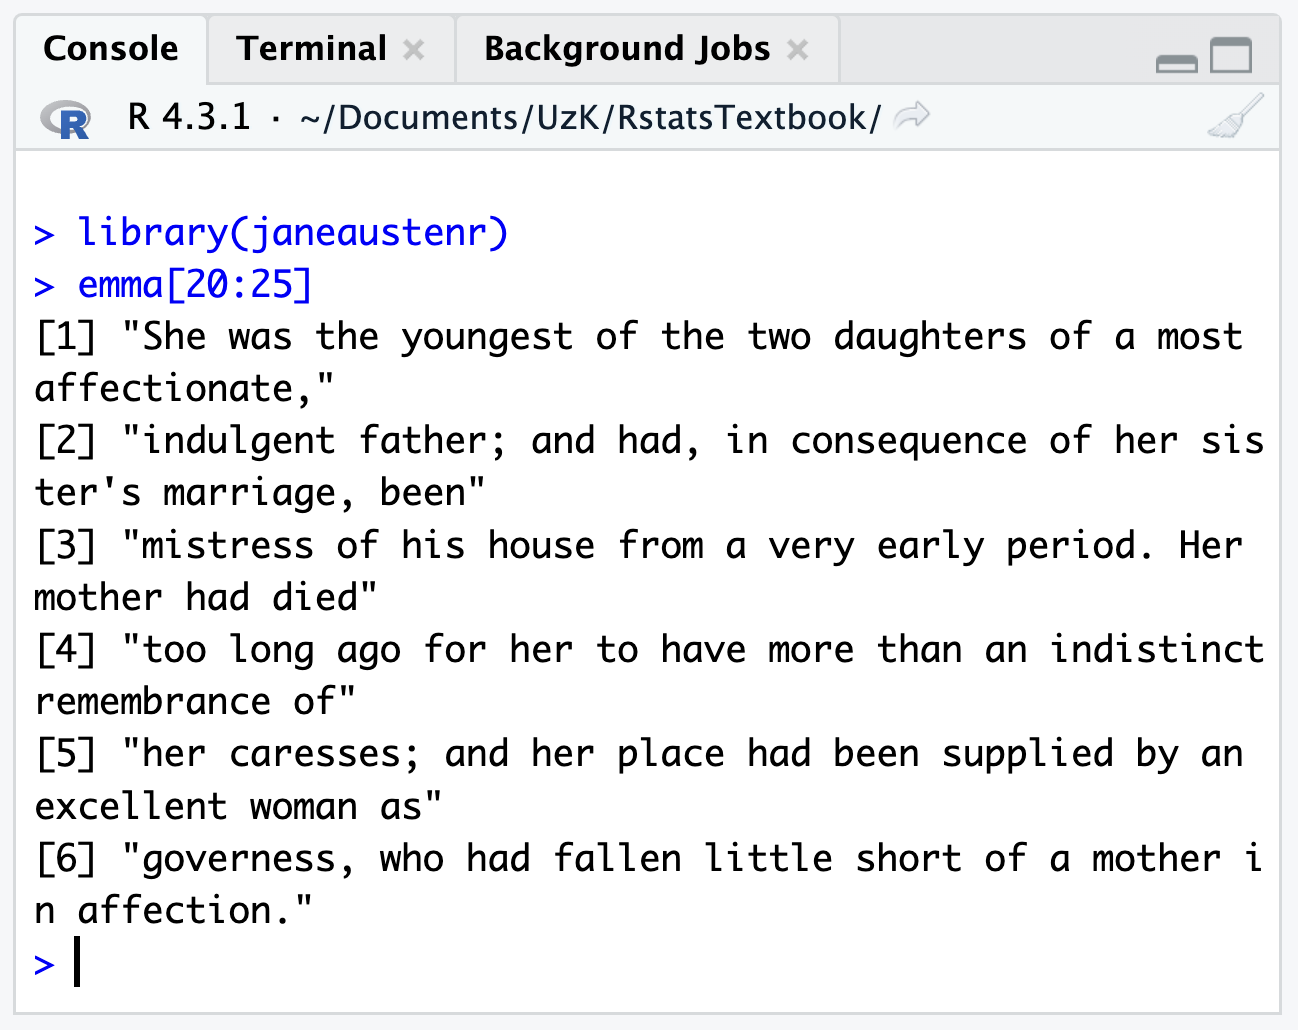
\includegraphics[width=4.16667in,height=\textheight]{images/Emma2025.png}

}

\caption{\label{fig-emma2025}Screenshot showing a selection of lines
from the object \texttt{emma} (note that you can adjust the size of the
Console pane to see more or less of the text at any one time).}

\end{figure}%

To find out more about a dataset or function within a package, use the
functions \texttt{help()} or \texttt{?}, e.g., \texttt{help(emma)} or
\texttt{?emma}. In this case, the help file provides us with a short
description of this object and a link to the original source from which
the package creator obtained the novel (which is in the
\href{https://www.gutenberg.org/help/faq.html\#what-books-does-project-gutenberg-publish}{public
domain}, otherwise it would not be possible to share it in this way).

\section{\texorpdfstring{Citing \texttt{R}
packages}{Citing R packages}}\label{citing-r-packages}

When we use a package that is not part of base \texttt{R}, it is very
important to reference the package adequately. There are two main
reasons for doing this. For a start, the people who create and maintain
these packages largely do so in their free time and they deserve full
credit for their incredibly valuable work and contribution to science.
Hence, whenever you use a package for your research, you should cite it,
just like you would other sources.

The help page of the \{janeaustenr\} package already informed us that
the maintainer of the package is Julia Silge. To get a full citation,
however, we should use the \texttt{citation()} function. Enter
\texttt{citation("janeaustenr")} in the Console to find out how to cite
this package.

Note that the recommended bibliographic reference also includes the
package version, which is important for reproducibility as the package
may evolve and someone wanting to reproduce your analysis (and this may
well be future you!) will need to know which version you used. This is
the second main reason why we should be diligent about citing the
packages that we used. In a research report, thesis, or academic
article, you could cite the \{janeaustenr\} package like this:

\begin{quote}
We used the \emph{janeaustenr} package (Silge 2022) to access Jane
Austen's six published novels in R (R Core Team 2024).
\end{quote}

You can see the full references by hovering on the in-text citation
links or by going to the
\href{https://elenlefoll.github.io/RstatsTextbook/references.html}{References}
section of this book.

\begin{tcolorbox}[enhanced jigsaw, breakable, colbacktitle=quarto-callout-note-color!10!white, bottomtitle=1mm, colframe=quarto-callout-note-color-frame, leftrule=.75mm, bottomrule=.15mm, colback=white, toptitle=1mm, rightrule=.15mm, title=\textcolor{quarto-callout-note-color}{\faInfo}\hspace{0.5em}{More about referencing packages}, coltitle=black, opacityback=0, arc=.35mm, left=2mm, titlerule=0mm, toprule=.15mm, opacitybacktitle=0.6]

You may also want to install the \{report\} package, which includes a
number of useful functions for citing \texttt{R} versions and \texttt{R}
packages:

\begin{Shaded}
\begin{Highlighting}[]
\NormalTok{report}\SpecialCharTok{::}\FunctionTok{report\_system}\NormalTok{()}
\end{Highlighting}
\end{Shaded}

\begin{verbatim}
Analyses were conducted using the R Statistical language (version 4.3.1; R Core
Team, 2023) on macOS Sonoma 14.4.1
\end{verbatim}

\begin{Shaded}
\begin{Highlighting}[]
\NormalTok{report}\SpecialCharTok{::}\FunctionTok{cite\_packages}\NormalTok{()}
\end{Highlighting}
\end{Shaded}

\begin{verbatim}
  - Makowski D, Lüdecke D, Patil I, Thériault R, Ben-Shachar M, Wiernik B (2023). "Automated Results Reporting as a Practical Tool to Improve Reproducibility and Methodological Best Practices Adoption." _CRAN_. <https://easystats.github.io/report/>.
  - Moroz G (2020). _Create check-fields and check-boxes with checkdown_. <https://CRAN.R-project.org/package=checkdown>.
  - R Core Team (2023). _R: A Language and Environment for Statistical Computing_. R Foundation for Statistical Computing, Vienna, Austria. <https://www.R-project.org/>.
  - Silge J (2022). _janeaustenr: Jane Austen's Complete Novels_. R package version 1.0.0, <https://CRAN.R-project.org/package=janeaustenr>.
  - Xie Y (2023). _knitr: A General-Purpose Package for Dynamic Report Generation in R_. R package version 1.45, <https://yihui.org/knitr/>. Xie Y (2015). _Dynamic Documents with R and knitr_, 2nd edition. Chapman and Hall/CRC, Boca Raton, Florida. ISBN 978-1498716963, <https://yihui.org/knitr/>. Xie Y (2014). "knitr: A Comprehensive Tool for Reproducible Research in R." In Stodden V, Leisch F, Peng RD (eds.), _Implementing Reproducible Computational Research_. Chapman and Hall/CRC. ISBN 978-1466561595.
\end{verbatim}

\begin{Shaded}
\begin{Highlighting}[]
\NormalTok{report}\SpecialCharTok{::}\FunctionTok{report\_packages}\NormalTok{()}
\end{Highlighting}
\end{Shaded}

\begin{verbatim}
  - report (version 0.5.8; Makowski D et al., 2023)
  - checkdown (version 0.0.12; Moroz G, 2020)
  - R (version 4.3.1; R Core Team, 2023)
  - janeaustenr (version 1.0.0; Silge J, 2022)
  - knitr (version 1.45; Xie Y, 2023)
\end{verbatim}

To find out more, it is also worth reading Steffi LaZerte's blog post on
``How to cite R and R packages'':
\url{https://ropensci.org/blog/2021/11/16/how-to-cite-r-and-r-packages/}.

\end{tcolorbox}

\bookmarksetup{startatroot}

\chapter{Getting staRted}\label{getting-started}

\subsubsection*{\texorpdfstring{\textbf{Chapter
overview}}{Chapter overview}}\label{chapter-overview-1}
\addcontentsline{toc}{subsubsection}{\textbf{Chapter overview}}

Now that you have installed and tested \texttt{R} and \texttt{RStudio},
in this chapter, you will learn how to:

\begin{itemize}
\tightlist
\item
  Use the \texttt{R} Console.
\item
  Do basic mathematical operations in \texttt{R}.
\item
  Create and use \texttt{R} objects.
\item
  Write and save \texttt{.R} scripts.
\item
  Add comments to your scripts.
\item
  Keep your cool when errors pop up! 😎
\end{itemize}

If you are already familiar with the basics of \texttt{R} and are keen
to learn more about doing statistics in \texttt{R}, you can skip most of
this chapter. That's said, it's probably not a bad idea to have a go at
the quiz questions and the final task to refresh your memory.

\section{Using the Console}\label{using-the-console}

{\marginnote{\begin{footnotesize}This is what you did in the previous
chapter when you tested that \texttt{RStudio} was working properly
(using the command: \texttt{plot(1:10)}).\end{footnotesize}}}

One way to write \texttt{R} code in \texttt{RStudio} is to use the
Console. If you set up \texttt{RStudio} as recommended
\href{https://elenlefoll.github.io/RstatsTextbook/InstallingR.html\#global-options}{here},
the Console should be in your top-right pane. You can type a line of
code immediately after the command prompt \texttt{\textgreater{}} and
press ``Enter''.

Data input is the most basic operation in \texttt{R}. Try inputting a
number by typing it out in the Console and then pressing ``Enter''.
\texttt{R} will interpret the number and return it. You can input both
integers (whole numbers, e.g., \texttt{13}) and decimal numbers (e.g.,
\texttt{0.5}).

\begin{figure}

\centering{

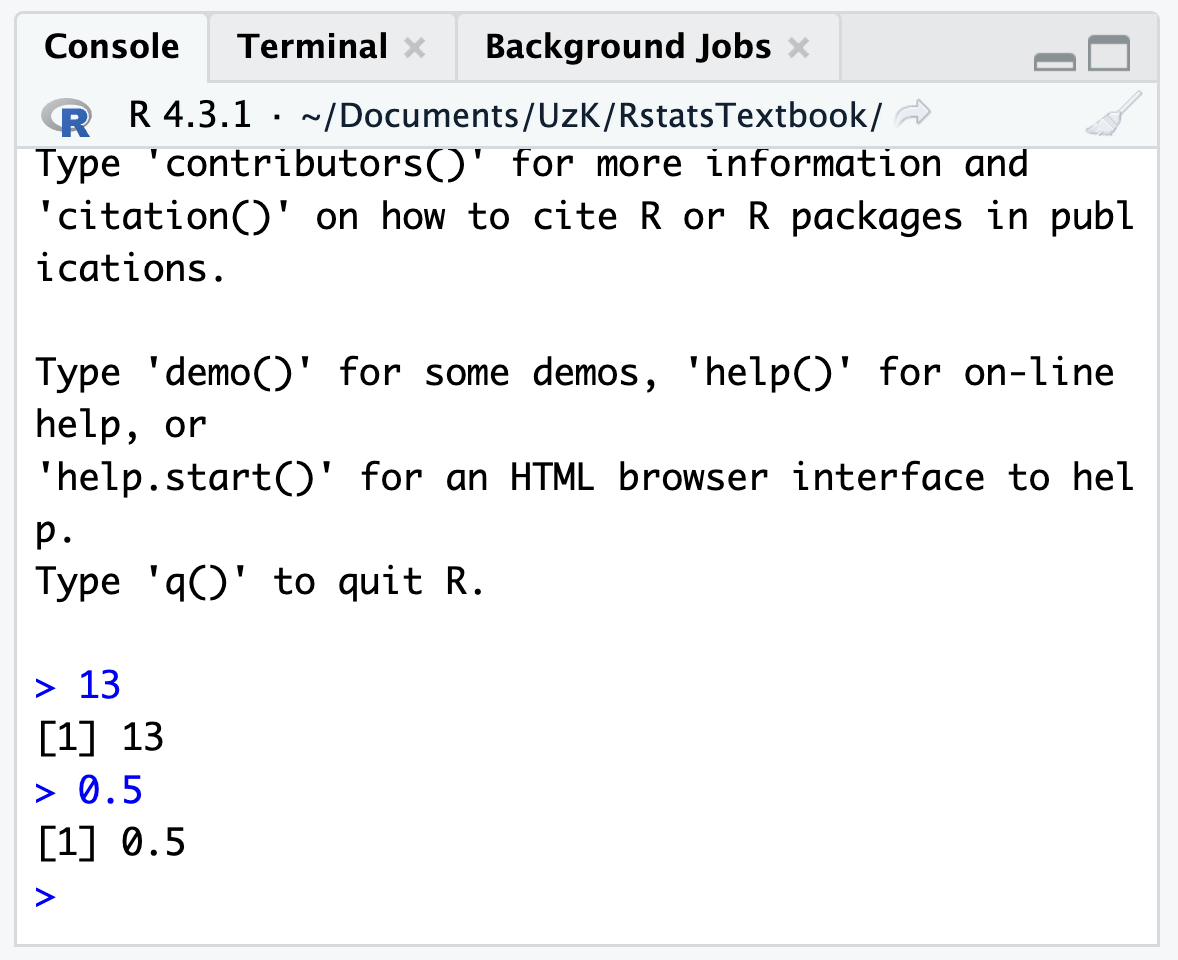
\includegraphics[width=4.6875in,height=\textheight]{images/ConsoleInputNumbers.png}

}

\caption{\label{fig-ConsoleInputNumbers}Inputting numbers in the
Console}

\end{figure}%

\texttt{R} can handle not only numbers but also text data, known as
``character strings'' or just ``strings''. Strings must always be
enclosed in quotation marks. You can choose to use either double
quotation marks \texttt{"\ "} or single quotation marks
\texttt{\textquotesingle{}\ \textquotesingle{}}, but it is important to
be consistent. In this textbook, we will use double quotation marks
throughout.

Try first inputting a single word and then an entire sentence in the
Console.

\begin{figure}

\centering{

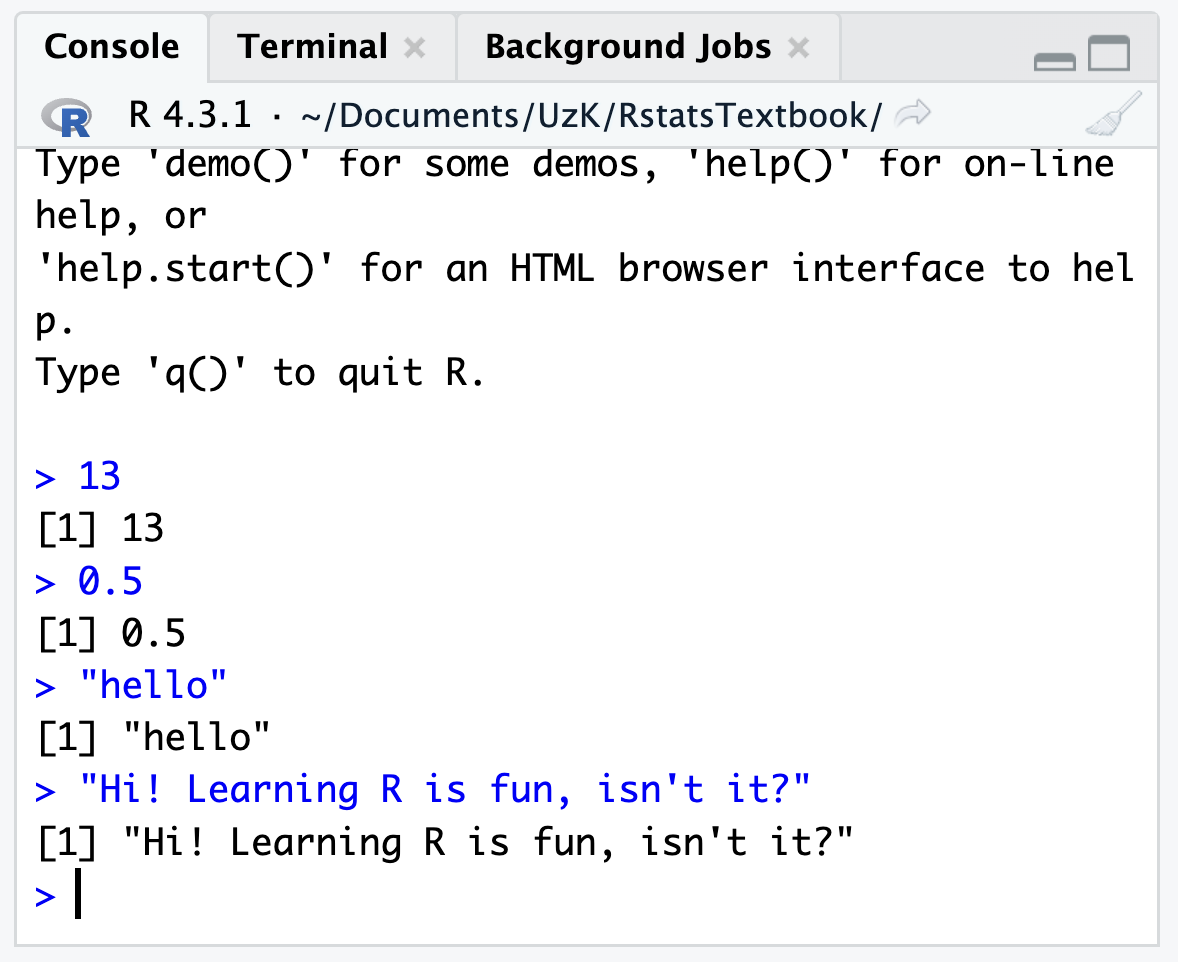
\includegraphics[width=4.6875in,height=\textheight]{images/ConsoleInputStrings.png}

}

\caption{\label{fig-ConsoleInputStrings}Inputting strings in the
Console}

\end{figure}%

\begin{tcolorbox}[enhanced jigsaw, breakable, colbacktitle=quarto-callout-tip-color!10!white, bottomtitle=1mm, colframe=quarto-callout-tip-color-frame, leftrule=.75mm, bottomrule=.15mm, colback=white, toptitle=1mm, rightrule=.15mm, title=\textcolor{quarto-callout-tip-color}{\faLightbulb}\hspace{0.5em}{Quiz time!}, coltitle=black, opacityback=0, arc=.35mm, left=2mm, titlerule=0mm, toprule=.15mm, opacitybacktitle=0.6]

1) What happens if you enter a word without quotation marks?

\end{tcolorbox}

\section{\texorpdfstring{Doing maths in
\texttt{R}}{Doing maths in R}}\label{doing-maths-in-r}

\texttt{R} can also be used as a very powerful calculator. The lines of
code in Figure~\ref{fig-ConsoleInputMathematicalOperations} demonstrate
mathematical operations involving addition (\texttt{+}), subtraction
(\texttt{-}), division (\texttt{/}), and multiplication (\texttt{*}).
Try out a few yourself!

\begin{figure}

\centering{

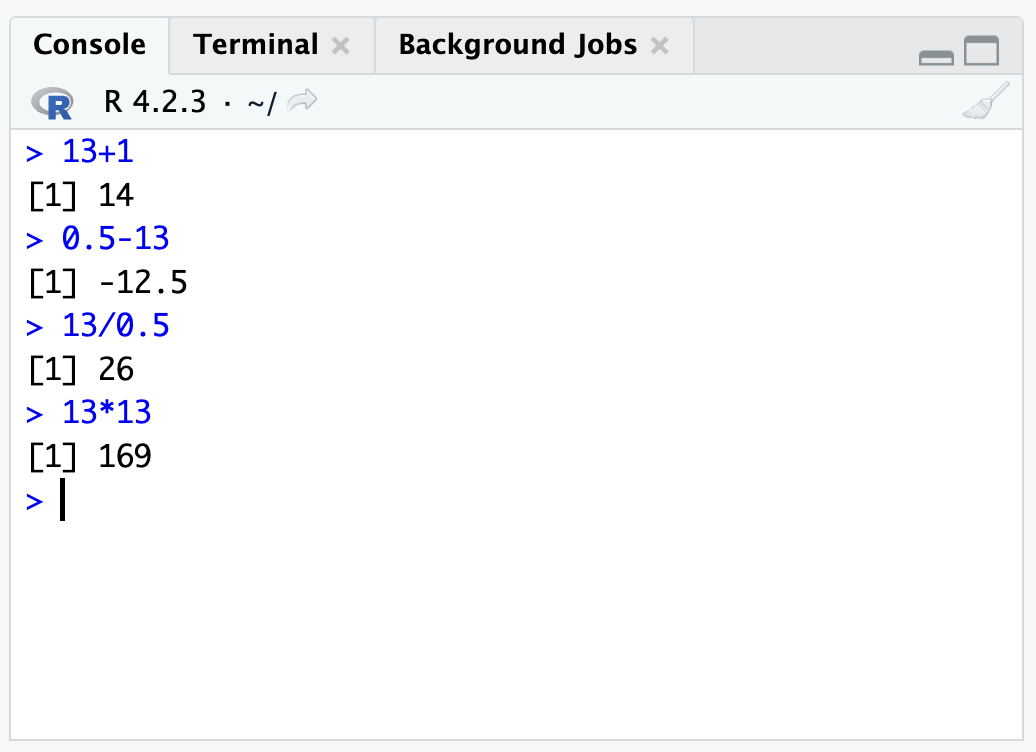
\includegraphics[width=4.6875in,height=\textheight]{images/ConsoleInputMathematicalOperations.png}

}

\caption{\label{fig-ConsoleInputMathematicalOperations}Using the
\texttt{R} Console as a calculator}

\end{figure}%

\begin{tcolorbox}[enhanced jigsaw, breakable, colbacktitle=quarto-callout-tip-color!10!white, bottomtitle=1mm, colframe=quarto-callout-tip-color-frame, leftrule=.75mm, bottomrule=.15mm, colback=white, toptitle=1mm, rightrule=.15mm, title=\textcolor{quarto-callout-tip-color}{\faLightbulb}\hspace{0.5em}{Quiz time!}, coltitle=black, opacityback=0, arc=.35mm, left=2mm, titlerule=0mm, toprule=.15mm, opacitybacktitle=0.6]

2) Try entering \texttt{13\^{}2} in the Console. What does the
\texttt{\^{}} (caret) operator do?

~

3) Compare \texttt{13*13} with \texttt{13\ *\ 13}. What is the
difference in the output?

\end{tcolorbox}

\section{\texorpdfstring{Working with \texttt{R}
objects}{Working with R objects}}\label{working-with-r-objects}

So far, we have used the Console like a calculator. It's important to
understand that, just like with a standard calculator, the output of all
of our operations was not saved anywhere.

\texttt{R} allows us to store values, sequences of values, and the
results of computations in so-called ``objects'' for later use. We use
the assignment operator (\texttt{\textless{}-}) to assign a value or
sequence of values to an object name.

Write out the following line to create an object called
\texttt{my.favourite.number} that contains your own favourite number.

\begin{Shaded}
\begin{Highlighting}[]
\NormalTok{my.favourite.number }\OtherTok{\textless{}{-}} \DecValTok{13}
\end{Highlighting}
\end{Shaded}

When you enter this line in the Console and press ``Enter'', it should
look like nothing happened: \texttt{R} does not return anything in the
Console. Instead, it saves the output in an object called
\texttt{my.favourite.number}. However, if you look in your Environment
pane, you should see that an object has appeared
(Figure~\ref{fig-ObjectCreation}).

\begin{figure}

\centering{

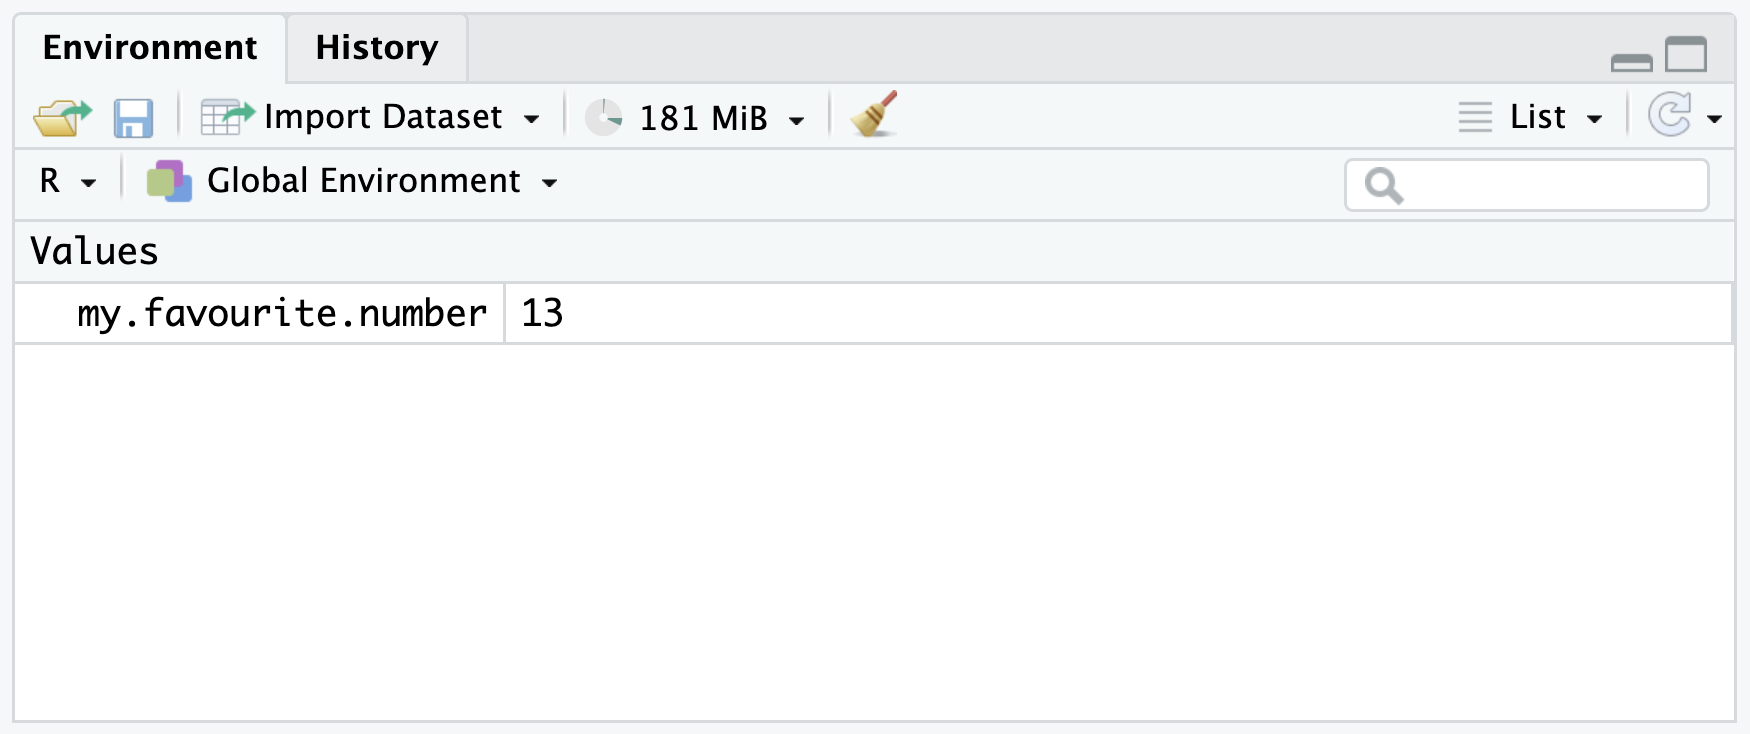
\includegraphics[width=5.72917in,height=\textheight]{images/ObjectCreation.png}

}

\caption{\label{fig-ObjectCreation}Created object in the Environment
pane}

\end{figure}%

To save an object containing a character string, we use quotation marks.
Create an object called \texttt{my.favourite.word} containing your
favourite word (in any written language of your choice).

\begin{Shaded}
\begin{Highlighting}[]
\NormalTok{my.favourite.word }\OtherTok{\textless{}{-}} \StringTok{"empathy"}
\end{Highlighting}
\end{Shaded}

Your Environment pane should now contain two objects. You can print the
content of a stored object by entering the object name in the Console
and then pressing ``Enter'' (see Figure~\ref{fig-ShowObjects}).

Tip: If you feeling lazy or simply want to avoid making a typo, you can
type only the first few letters of an object name and then press the
``Tab'' key (\texttt{↹} or \texttt{⇥}). \texttt{RStudio} will then give
you a drop-down menu with possible options. Select the one you want by
clicking on it or pressing ``Enter''.

\begin{figure}

\centering{

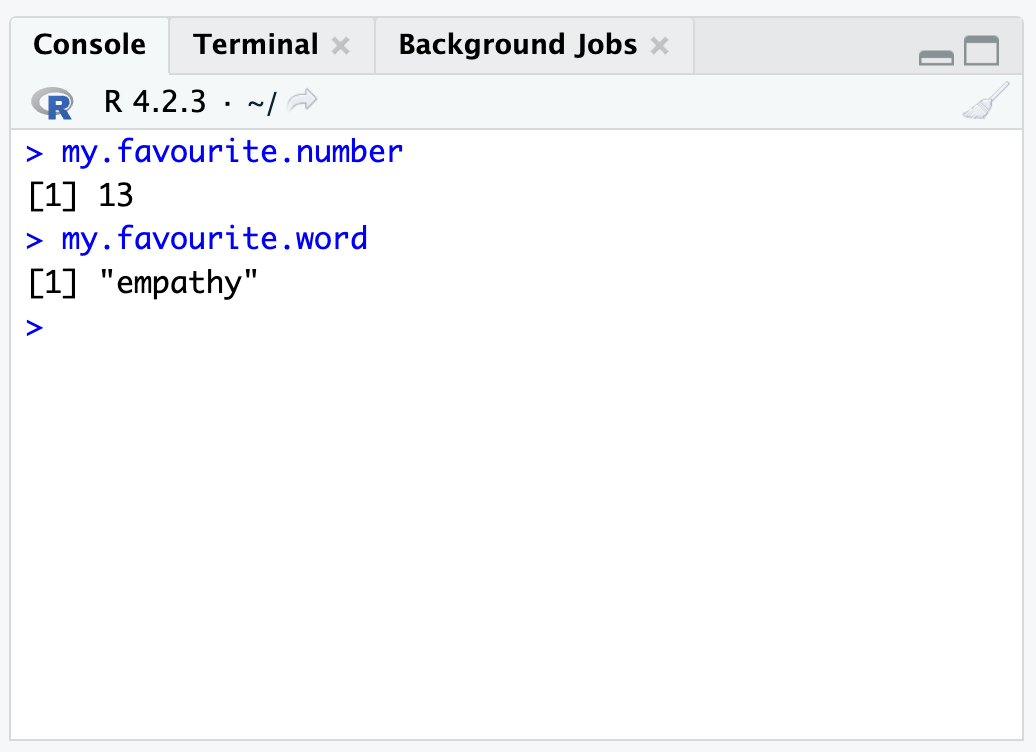
\includegraphics[width=4.6875in,height=\textheight]{images/ShowObjects.png}

}

\caption{\label{fig-ShowObjects}Calling up stored objects in the Console
to view their content}

\end{figure}%

These two objects are of different types. We can use the
\texttt{class()} function to find out which type of object an object is.

\begin{figure}

\centering{

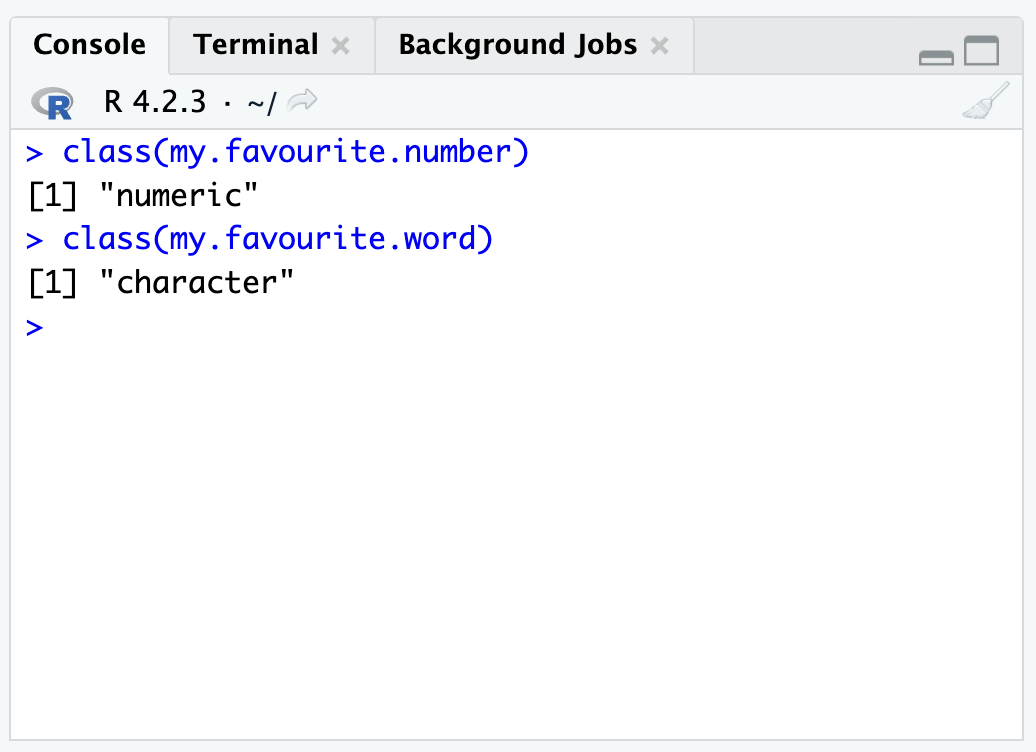
\includegraphics[width=4.6875in,height=\textheight]{images/ShowObjectClass.png}

}

\caption{\label{fig-ShowObjectClass}Using the \texttt{class()} function}

\end{figure}%

Here, \texttt{my.favourite.number} is a numeric object, while
\texttt{my.favourite.word} is a character object.

Object naming conventions in \texttt{R} are fairly flexible. We can use
dots (\texttt{.}), underscores (\texttt{\_}) and capital letters to make
our object names maximally informative and easy for us humans to read.
However, spaces and other symbols are not allowed. All of these options
work:

\begin{Shaded}
\begin{Highlighting}[]
\NormalTok{word2 }\OtherTok{\textless{}{-}} \StringTok{"cheerful"}
\NormalTok{my.second.word }\OtherTok{\textless{}{-}} \StringTok{"cheerful"}
\NormalTok{my\_second\_word }\OtherTok{\textless{}{-}} \StringTok{"cheerful"}
\NormalTok{MySecondWord }\OtherTok{\textless{}{-}} \StringTok{"cheerful"}
\end{Highlighting}
\end{Shaded}

\begin{figure}

\centering{

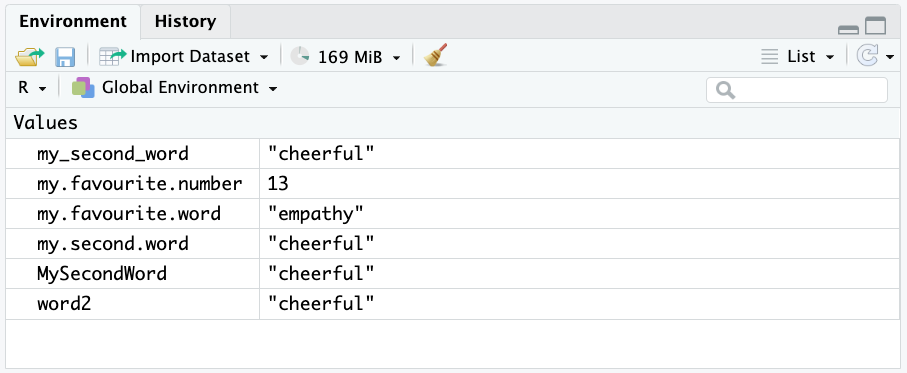
\includegraphics[width=5.72917in,height=\textheight]{images/MultipleObjectsEnvironmentPane.png}

}

\caption{\label{fig-MultipleObjectsEnvironmentPane}Environment pane
showing all of the objects currently stored in the \texttt{R} session
environment}

\end{figure}%

\begin{tcolorbox}[enhanced jigsaw, breakable, colbacktitle=quarto-callout-tip-color!10!white, bottomtitle=1mm, colframe=quarto-callout-tip-color-frame, leftrule=.75mm, bottomrule=.15mm, colback=white, toptitle=1mm, rightrule=.15mm, title=\textcolor{quarto-callout-tip-color}{\faLightbulb}\hspace{0.5em}{Quiz time!}, coltitle=black, opacityback=0, arc=.35mm, left=2mm, titlerule=0mm, toprule=.15mm, opacitybacktitle=0.6]

4) Which of these object names are \emph{not} allowed in \texttt{R}? Try
to create an object with each of these names and see if you get an error
message or not.

\end{tcolorbox}

Object names should not contain spaces or symbols like \texttt{!}, nor
should they contain hyphens as the hyphen is reserved for the
mathematical operator ``minus''. Digits can be used anywhere except at
the beginning of an object name. And whilst it is possible to have
special characters such as accented letters like ``è'', it is not
recommended that you use them for object names.

Object names are unique. If you create a new object with an existing
object name, it will overwrite the existing object with the new one. In
other words, you will lose the values that you saved in the original
object. Try it out by running this line and observing what happens in
your Environment pane:

\begin{Shaded}
\begin{Highlighting}[]
\NormalTok{word2 }\OtherTok{\textless{}{-}} \StringTok{"surprised"}
\end{Highlighting}
\end{Shaded}

Earlier on, you created an object called \texttt{word2} which contained
the string ``cheerful''. But, by running this new line of code,
``cheerful'' has been replaced by the string ``surprised'' - with no
warning that you were about to permanently delete ``cheerful''! 😲

The command to delete a single object from your environment is
\texttt{remove()} or \texttt{rm()}. Hence, to permanently delete the
object \texttt{MySecondWord}, you can use either of these commands:

\begin{Shaded}
\begin{Highlighting}[]
\FunctionTok{remove}\NormalTok{(MySecondWord)}
\FunctionTok{rm}\NormalTok{(MySecondWord)}
\end{Highlighting}
\end{Shaded}

\section{\texorpdfstring{Writing and saving \texttt{.R}
scripts}{Writing and saving .R scripts}}\label{writing-and-saving-.r-scripts}

If we shut down \texttt{Rstudio} right now, we will lose all of our work
so far. This is because the objects that we have created are only saved
in the environment of our current \texttt{R} session. Whilst this might
sound reckless, it is actually a good thing: In the previous chapter, we
set our Global Options settings in \texttt{RStudio} such that, whenever
we restart \texttt{RStudio}, we begin with a clean slate, or a perfectly
clean and tidy kitchen. We don't want any dirty dishes or stale
ingredients lying around when we enter the kitchen! With this in mind,
close \texttt{RStudio} now and open it again to start a new \texttt{R}
session.

You should now have an empty history in your Console pane and an empty
Environment pane. Whilst nobody wants to start cooking in a messy
kitchen, it's also true that, if we want to remember what we did in a
previous cooking/baking session, we should write it down. The pages of
our recipe book are \texttt{.R} scripts. In the following, we will see
that writing scripts is much better than running everything from the
Console. It allows us to save and rerun our entire analysis pipeline any
time we want. It also ensures that our analyses are reproducible and
saves us time as we don't have to rewrite our code every time.
Crucially, if we made a mistake at any stage, we can go back and correct
it and rerun the entire corrected script at the click of a button.

There are three ways to create a new \texttt{.R} script in
\texttt{RStudio}. Pick the one that you like best:

\begin{enumerate}
\def\labelenumi{\arabic{enumi}.}
\tightlist
\item
  Navigate to the top menu item ``File'', then select ``New File'', then
  click on ``R Script''.
\item
  Click on the icon with a white page and a green plus button in the top
  left corner of the tool bar.
\item
  Use the keyboard shortcut \texttt{Shift\ +\ Ctrl/Cmd\ +\ N}.
\end{enumerate}

Whichever option you chose, \texttt{RStudio} should have opened an empty
file in a fourth pane. This is the ``Source pane'' and it should have
appeared in the top-left corner of your \texttt{RStudio} window.

We can now type our code in this empty \texttt{.R} script in the Source
pane, just like we did in the Console. Type the following lines of code:

\begin{Shaded}
\begin{Highlighting}[]
\DecValTok{13}\SpecialCharTok{*}\DecValTok{13}
\NormalTok{my.favourite.number }\OtherTok{\textless{}{-}} \DecValTok{13}
\NormalTok{my.favourite.word }\OtherTok{\textless{}{-}} \StringTok{"empathy"}
\end{Highlighting}
\end{Shaded}

You will have noticed that when you pressed ``Enter'' after every line,
nothing happened: Nowhere can we see the result of \texttt{13*13}, nor
have our two objects been saved to the environment as Environment pane
remains empty (see Figure~\ref{fig-NewScript}). Just like a recipe for a
cake is not an actual, delicious cake, but simply a set of instructions,
a script is only a text file that contains lines of code as
instructions. For these instructions to be executed, we need to send
them to the \texttt{R} Console where they will be interpreted as
\texttt{R} code.

\begin{figure}

\centering{

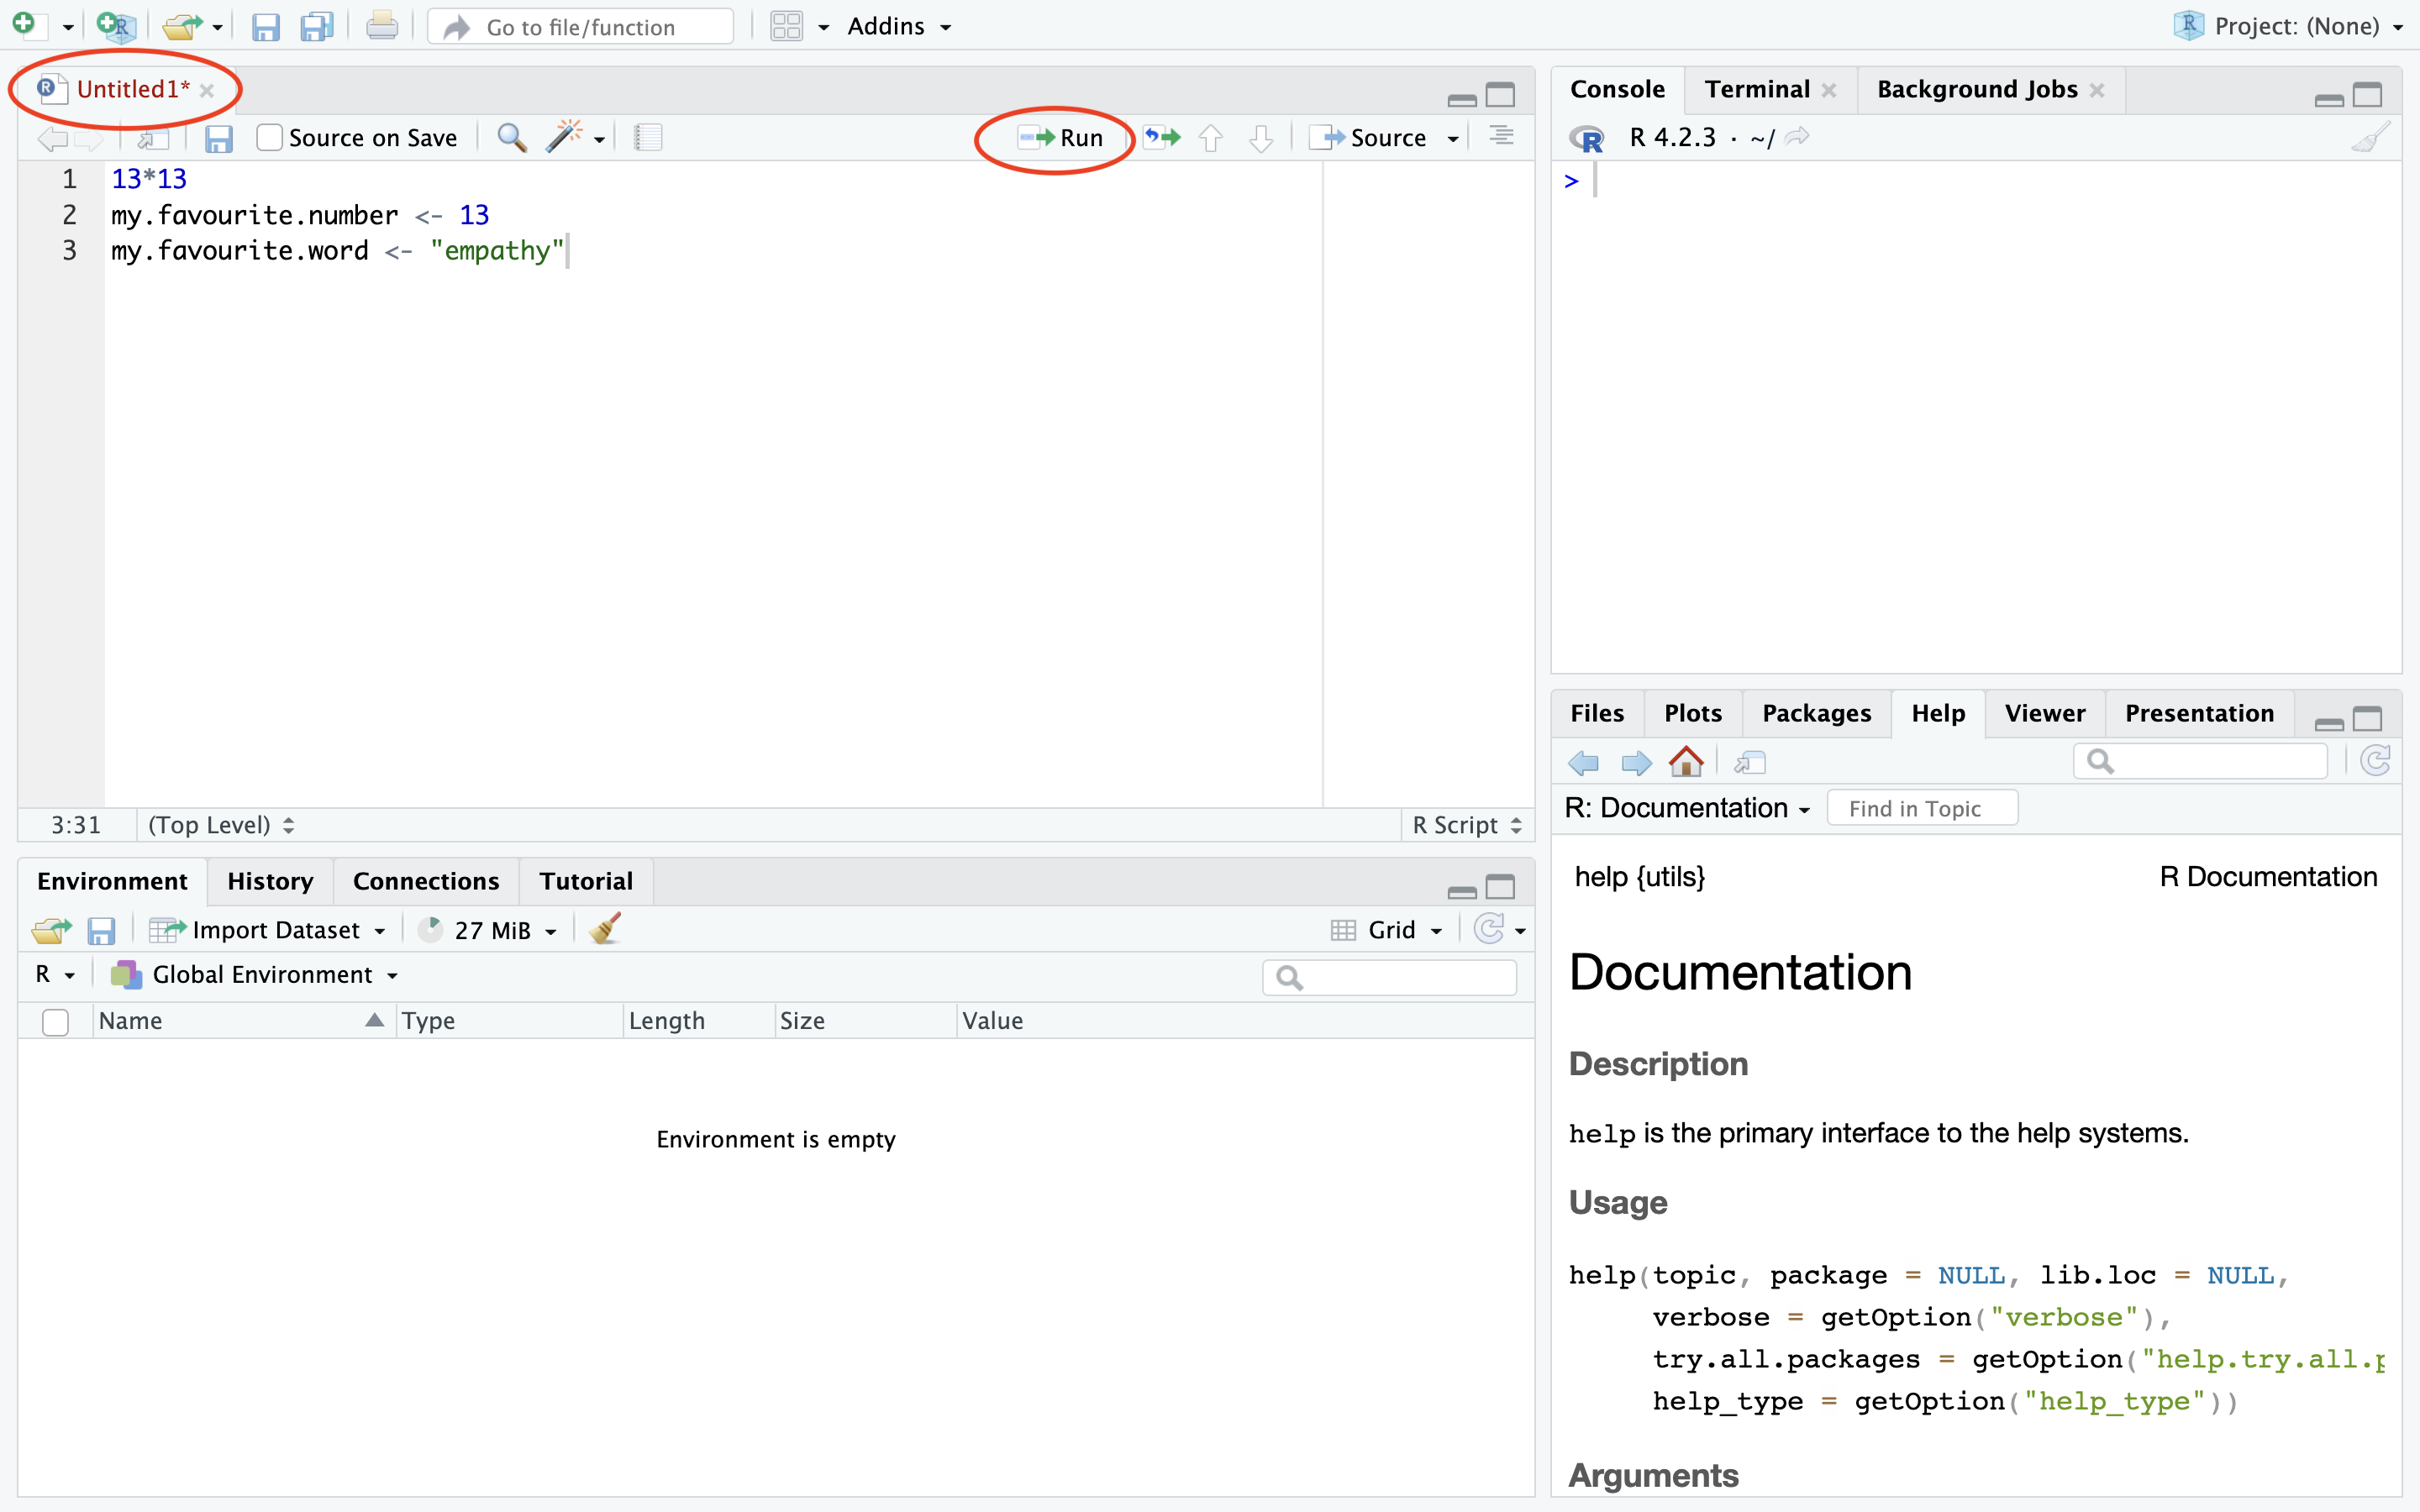
\includegraphics{images/NewScript.png}

}

\caption{\label{fig-NewScript}Writing code in a script}

\end{figure}%

To send a line of code to the Console, or ``run'' a line of code, select
the line that you want to run, or place your mouse cursor anywhere
within that line and then click on the `Run' button (in the top-right
corner of the pane, see Figure~\ref{fig-NewScript}) or use the keyboard
shortcut \texttt{Ctrl/Cmd\ +\ Enter}.

Run the three lines of code of your script using these two options and
check that a) you are seeing the result of the mathematical operation in
the Console output and b) two objects have been added to your
environment.

It is now very easy to rerun this script any time we want to redo this
calculation and recreate these two \texttt{R} objects. However, our
\texttt{.R} script is not yet saved! \texttt{RStudio} is warning us
about this by highlighting the file name ``Untitled1*'' in red (see
Figure~\ref{fig-NewScript}). Just like with any unsaved computer file,
if we were to shut \texttt{RStudio} down now, we would loose our work.
So, let us save this \texttt{.R} script locally, that is on our own
computer. To do so either:

\begin{enumerate}
\def\labelenumi{\arabic{enumi}.}
\tightlist
\item
  Navigate to the top menu item ``File'' and then click on ``Save'',
\item
  Click on the save icon 💾, or
\item
  Use the keyboard shortcut \texttt{Ctrl/Cmd+\ S}.
\end{enumerate}

Give your script a meaningful file name. Remember that file names should
be both computer-readable and human-readable. If you navigate to the
folder where you saved your \texttt{.R} script, you should see that its
file extension is \texttt{.R}. You should also see that it is a tiny
file because it contains nothing more than a few lines of text. If you
double click on an \texttt{.R} file, \texttt{RStudio} should
automatically open it. However, if you wanted, you could open
\texttt{.R} files with any text-processing software, such as LibreOffice
Writer or Microsoft Word.

\subsection{Writing comments}\label{writing-comments}

Just like in a recipe book, in addition to writing the actual
instructions, we can also write some notes, for example to remind
ourselves of why we did things in a particular way or for what occasion
we created a special dish. In programming, notes are called ``comments''
and they are typically preceded by the \texttt{\#} symbol.

Thus, if a line starts with a \texttt{\#} symbol, we say that it is
``commented out''. \texttt{RStudio} helpfully displays lines that are
commented out in a different colour. These lines will not be interpreted
as code even if you send them to the Console. Write the following lines
in your script and try to run them.

\begin{Shaded}
\begin{Highlighting}[]
\CommentTok{\#13\^{}13}

\CommentTok{\#StringObject3 \textless{}{-} "This line has been commented out so the object will not be saved in the environment even if you try to run it."}
\end{Highlighting}
\end{Shaded}

As you can see, nothing happens. You can also add comments next to a
line of interpretable code. In this case, the code is interpreted up
until the \texttt{\#}. This can be helpful to make a note of what a line
of code does, e.g.:

\begin{Shaded}
\begin{Highlighting}[]
\FunctionTok{sqrt}\NormalTok{(}\DecValTok{169}\NormalTok{) }\CommentTok{\# Here the sqrt() function will compute the square root of 169.}
\end{Highlighting}
\end{Shaded}

It is good practice to comment your code when working in an \texttt{.R}
script. Comments are crucial for other people to understand what your
code does and how it achieves that. But even if you are confident that
you are the only person who will ever use your code, it is still a very
good idea to use comments to make notes documenting your intentions and
your reasoning as you write your script.

Finally, writing comments in your code as you work through the examples
in this book is a great way to reinforce what you are learning. From
this chapter onwards, I recommend that, for each chapter, you create an
\texttt{.R} script documenting what you have learnt, adding lots of
comments to help you remember how things work. This is generally more
efficient (and less error-prone!) than trying to take notes in a
separate document (e.g., in a Microsoft Word file) or on paper.

\section{Using relational operators}\label{using-relational-operators}

Now that we have saved some objects in our environment, we can use them
in calculations. Try out the following operations (and any other that
take your fancy) with your own favourite number:

\begin{Shaded}
\begin{Highlighting}[]
\NormalTok{my.favourite.number }\SpecialCharTok{/} \DecValTok{2}
\end{Highlighting}
\end{Shaded}

\begin{verbatim}
[1] 6.5
\end{verbatim}

\begin{Shaded}
\begin{Highlighting}[]
\NormalTok{my.favourite.number}\SpecialCharTok{*}\NormalTok{my.favourite.number}
\end{Highlighting}
\end{Shaded}

\begin{verbatim}
[1] 169
\end{verbatim}

\begin{Shaded}
\begin{Highlighting}[]
\FunctionTok{sqrt}\NormalTok{(my.favourite.number)}
\end{Highlighting}
\end{Shaded}

\begin{verbatim}
[1] 3.605551
\end{verbatim}

\begin{Shaded}
\begin{Highlighting}[]
\FunctionTok{sqrt}\NormalTok{(my.favourite.number}\SpecialCharTok{*}\NormalTok{my.favourite.number)}
\end{Highlighting}
\end{Shaded}

\begin{verbatim}
[1] 13
\end{verbatim}

We can also use relational operators such \texttt{\textgreater{}},
\texttt{\textless{}}, \texttt{\textless{}=}, \texttt{\textgreater{}=},
\texttt{==} and \texttt{!=} to make comparisons. Experiment with the
following commands to understand what these relational operators do:

\begin{Shaded}
\begin{Highlighting}[]
\NormalTok{my.favourite.number }\SpecialCharTok{\textgreater{}} \DecValTok{10}
\NormalTok{my.favourite.number }\SpecialCharTok{\textless{}} \DecValTok{10}
\NormalTok{my.favourite.number }\SpecialCharTok{==} \DecValTok{25}
\NormalTok{my.favourite.number }\SpecialCharTok{\textgreater{}=} \DecValTok{13}
\NormalTok{my.favourite.number }\SpecialCharTok{\textless{}=} \SpecialCharTok{{-}}\DecValTok{13}
\NormalTok{my.favourite.number }\SpecialCharTok{!=} \DecValTok{25}
\end{Highlighting}
\end{Shaded}

\begin{tcolorbox}[enhanced jigsaw, breakable, colbacktitle=quarto-callout-tip-color!10!white, bottomtitle=1mm, colframe=quarto-callout-tip-color-frame, leftrule=.75mm, bottomrule=.15mm, colback=white, toptitle=1mm, rightrule=.15mm, title=\textcolor{quarto-callout-tip-color}{\faLightbulb}\hspace{0.5em}{Quiz time!}, coltitle=black, opacityback=0, arc=.35mm, left=2mm, titlerule=0mm, toprule=.15mm, opacitybacktitle=0.6]

5) What is the relational operator that checks whether a value is ``more
than or equal to'' another value?

~

6) What is the relational operator that checks whether a value ``is not
equal to'' another value?

\end{tcolorbox}

The relational operators \texttt{==} and \texttt{!=} can also be used
with character objects. Find out how they work by first creating a new
character object with a word that was added to the 2025 edition of the
\emph{Petit Larousse} dictionary:

\begin{Shaded}
\begin{Highlighting}[]
\NormalTok{New.French.Word }\OtherTok{\textless{}{-}} \StringTok{"écogeste"}
\end{Highlighting}
\end{Shaded}

Then copy these lines of code to test how these relational operators
work with string characters.

\begin{Shaded}
\begin{Highlighting}[]
\NormalTok{New.French.Word }\SpecialCharTok{==} \StringTok{"écogeste"} 
\NormalTok{New.French.Word }\SpecialCharTok{!=} \StringTok{"trottinettiste"}
\end{Highlighting}
\end{Shaded}

\begin{tcolorbox}[enhanced jigsaw, breakable, colbacktitle=quarto-callout-tip-color!10!white, bottomtitle=1mm, colframe=quarto-callout-tip-color-frame, leftrule=.75mm, bottomrule=.15mm, colback=white, toptitle=1mm, rightrule=.15mm, title=\textcolor{quarto-callout-tip-color}{\faLightbulb}\hspace{0.5em}{Quiz time!}, coltitle=black, opacityback=0, arc=.35mm, left=2mm, titlerule=0mm, toprule=.15mm, opacitybacktitle=0.6]

7) Why does this line of code return \texttt{FALSE} even though
\texttt{New.French.Word} was assigned the character string ``écogeste''?

\begin{Shaded}
\begin{Highlighting}[]
\NormalTok{New.French.Word }\SpecialCharTok{==} \StringTok{"ecogeste"}
\end{Highlighting}
\end{Shaded}

\begin{verbatim}
[1] FALSE
\end{verbatim}

~

8) Why does this line of code return \texttt{FALSE} even though
\texttt{New.French.Word} was assigned the character string ``écogeste''?

\begin{Shaded}
\begin{Highlighting}[]
\NormalTok{New.French.Word }\SpecialCharTok{==} \StringTok{" écogeste"}
\end{Highlighting}
\end{Shaded}

\begin{verbatim}
[1] FALSE
\end{verbatim}

~

9) Why does this line of code return \texttt{FALSE} even though
\texttt{New.French.Word} was assigned the character string ``écogeste''?

\begin{Shaded}
\begin{Highlighting}[]
\NormalTok{New.French.Word }\SpecialCharTok{==} \StringTok{"Écogeste"}
\end{Highlighting}
\end{Shaded}

\begin{verbatim}
[1] FALSE
\end{verbatim}

~

10) Why does this line of code return \texttt{FALSE} even though
\texttt{New.French.Word} was assigned the character string ``écogeste''?

\begin{Shaded}
\begin{Highlighting}[]
\NormalTok{New.French.Word }\SpecialCharTok{!=} \StringTok{"écogeste"}
\end{Highlighting}
\end{Shaded}

\begin{verbatim}
[1] FALSE
\end{verbatim}

\end{tcolorbox}

\section{Dealing with errors}\label{dealing-with-errors}

When \texttt{R} cannot interpret your code, the Console will display an
error message in red. A large part of learning to code is really about
learning how to interpret these error messages and developing an
intuition for the most common reasons why errors occur.

\begin{figure}

\centering{

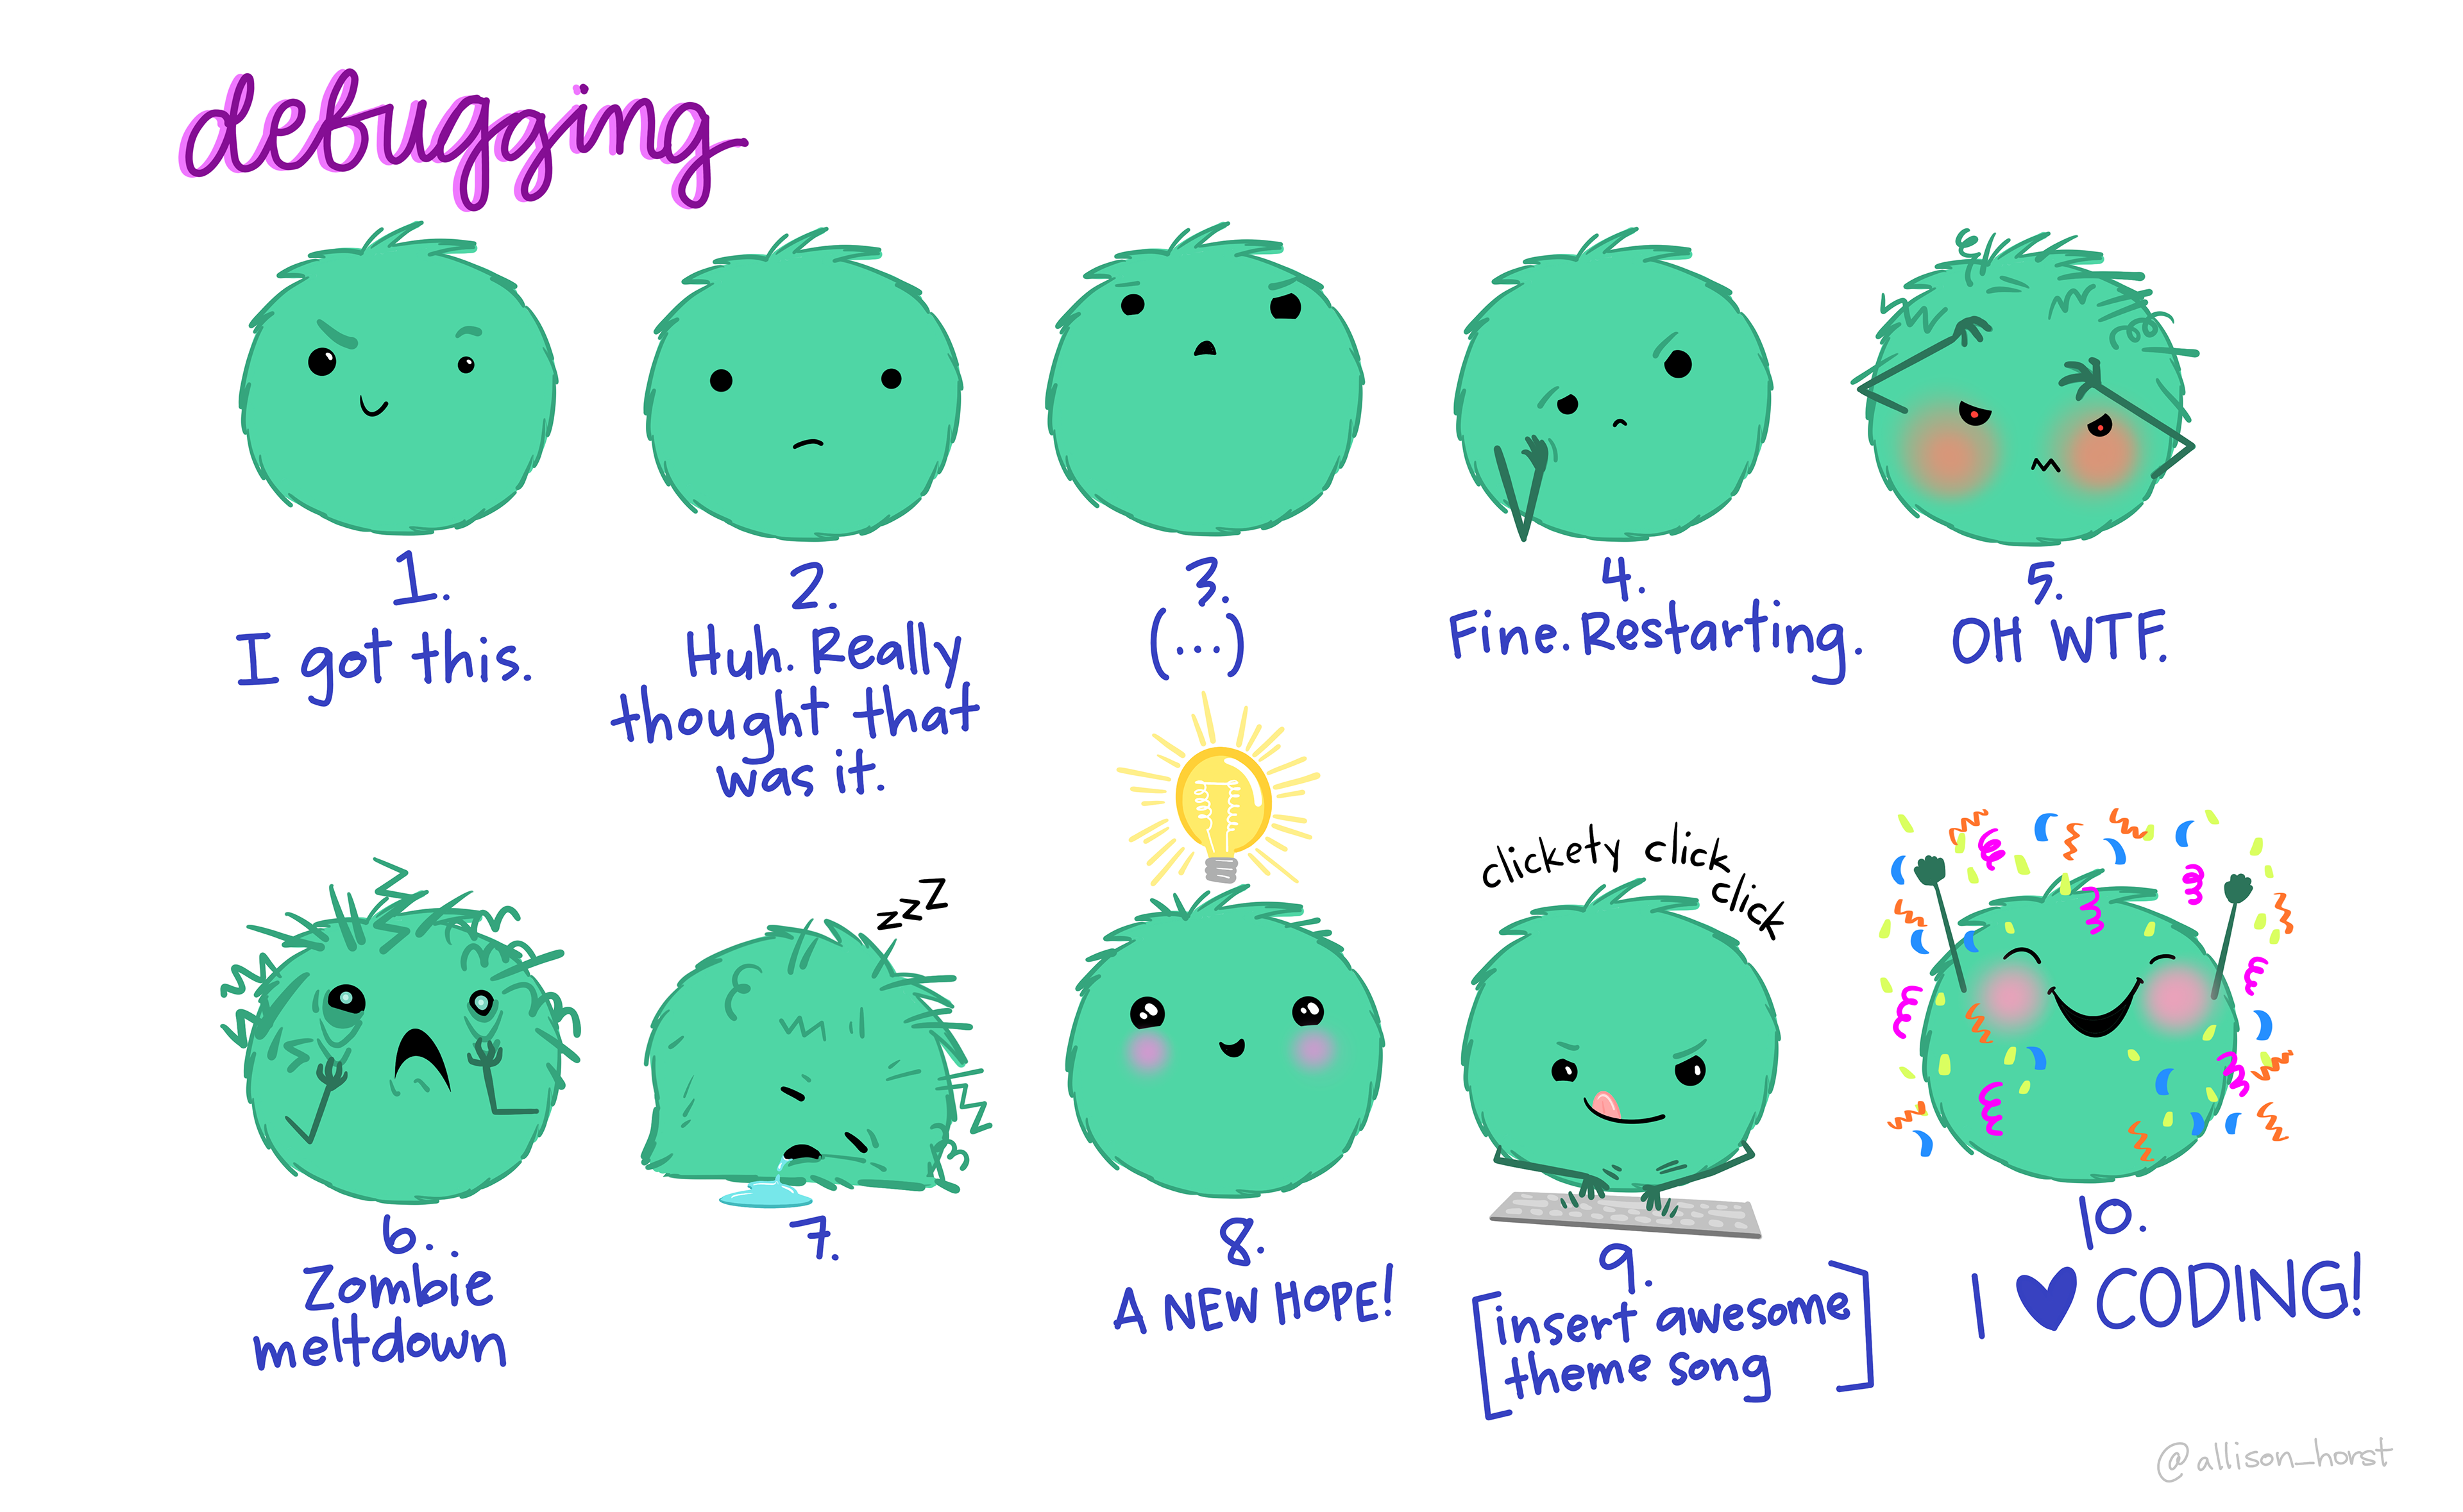
\includegraphics{images/DebuggingMonsters.png}

}

\caption{\label{fig-DebuggingMonster}The process of fixing programming
errors is called ``debugging'' and often involves an array of emotions
(artwork by
\href{https://allisonhorst.com/allison-horst}{@allison\_horst}).}

\end{figure}%

As you begin your journey learning to code in \texttt{R}, you are very
likely to encounter one problem on a regular basis. So let's take a
closer look at that error. Copy and paste this exact line of code and
try to run it in your \texttt{R} Console:

\begin{Shaded}
\begin{Highlighting}[]
\FunctionTok{sqrt}\NormalTok{(my.favourite.number}
\end{Highlighting}
\end{Shaded}

Notice that, in this erroneous line of code, we have (intentionally)
forgotten to include the final bracket. As a result, after you hit
``Enter'', the Console output shows a ``\texttt{+}'' instead of the
result of the mathematical operation. The ``\texttt{+}'' indicates that
the line is incomplete and therefore cannot be interpreted yet.
\texttt{R} is therefore asking you to complete your line of code.

\begin{figure}

\centering{

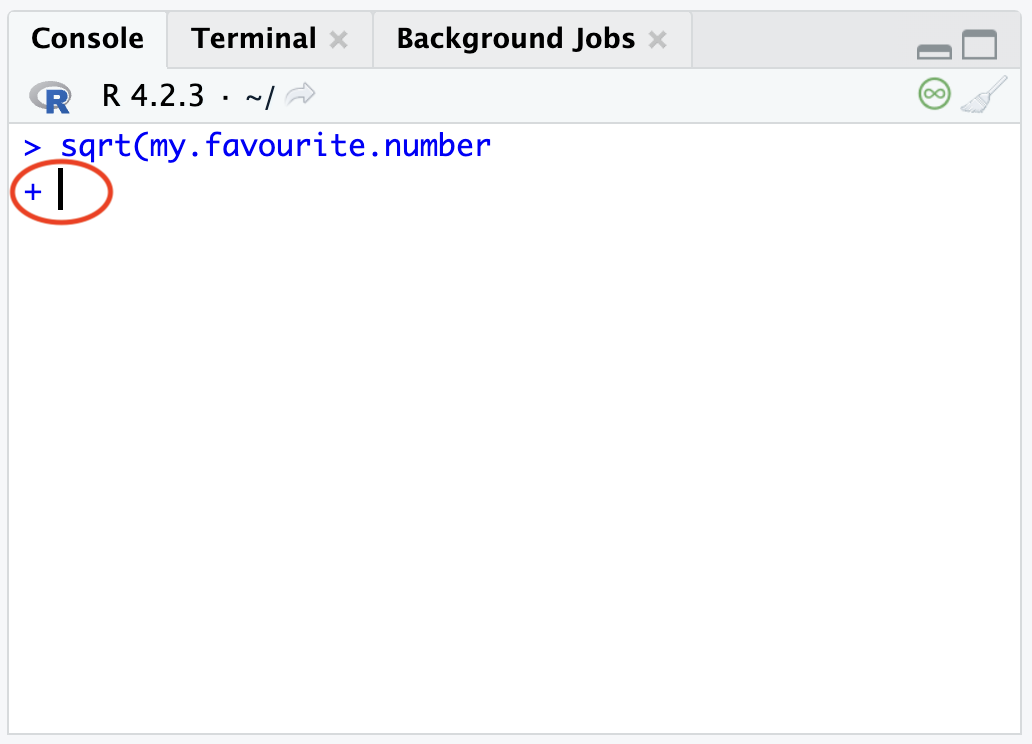
\includegraphics[width=4.6875in,height=\textheight]{images/ConsoleUncompleteFunction.png}

}

\caption{\label{fig-ConsoleUncompleteFunction}Incomplete function in
console}

\end{figure}%

There are two ways to fix this. The first method is to complete the line
of code directly in the Console. In this case, this means adding the
closing bracket ``\texttt{)}'' after the ``\texttt{+}'' and hitting
``Enter''. Now that the line has been completed, \texttt{R} is able to
interpret it as an \texttt{R} command and will output the result of the
operation.

If you are running a line of code just once, from the Console, this
first method is fine. As we have seen above, however, most of the time,
you will write your code in a script rather than in the Console. So this
first, on-the-fly, method is only recommendable for lines of code that
you will genuinely only need once. These include commands to install
packages, like \texttt{install.packages("janeaustenr")}, or to get
consult documentation files, e.g., \texttt{help(janeaustenr)}.

Given that we will mostly be working in scripts, let's now generate this
error from an \texttt{.R} script. To do so, copy and paste the erroneous
line of code in your \texttt{.R} script and try to run it by either
clicking on the ``Run'' icon or using the shortcut
\texttt{Ctrl/Cmd\ +\ Enter}:

\begin{Shaded}
\begin{Highlighting}[]
\FunctionTok{sqrt}\NormalTok{(my.favourite.number}
\end{Highlighting}
\end{Shaded}

Again, our incomplete line of code cannot be interpreted and the
``\texttt{+}'' symbol appears in the Console. Now, correct the error in
your script by adding the missing ``\texttt{)}'' and try to run the
command again:

\begin{Shaded}
\begin{Highlighting}[]
\FunctionTok{sqrt}\NormalTok{(my.favourite.number)}
\end{Highlighting}
\end{Shaded}

Even though we have corrected the problem, we now get an error! 🤯 At
first sight, this does not make sense, but look carefully at what
happened in the Console: The line of code that \texttt{R} tried to
interpret is
\texttt{sqrt(my.favourite.number\ +\ sqrt(my.favourite.number)}, i.e.,
the combination of the incomplete version of the command plus the
complete one. This is obviously nonsense and \texttt{R} tells us so by
outputting an error message!

\begin{figure}

\centering{

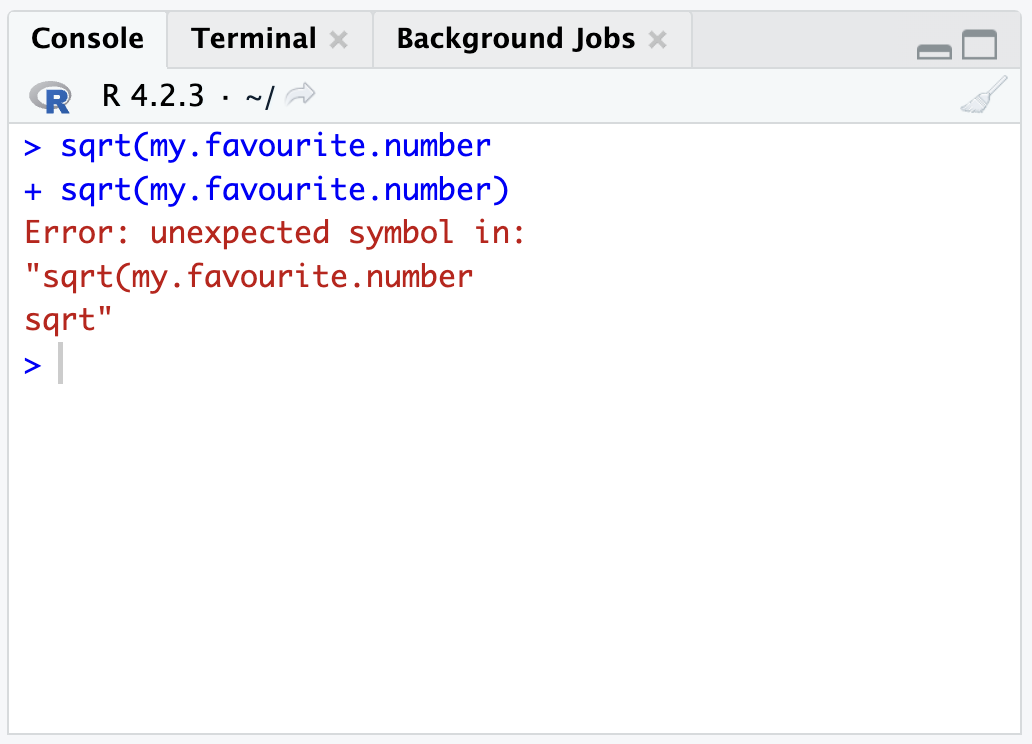
\includegraphics[width=4.6875in,height=\textheight]{images/ConsoleError.png}

}

\caption{\label{fig-ConsoleError}Error message in console}

\end{figure}%

To be able to enter a new line of code, we must see the command prompt
\texttt{\textgreater{}} in the Console. So, let's generate the error
again and learn how to fix it with the second method. Add this erroneous
line to your script again and run it:

\begin{Shaded}
\begin{Highlighting}[]
\FunctionTok{sqrt}\NormalTok{(my.favourite.number}
\end{Highlighting}
\end{Shaded}

The \texttt{+} situation arises again, but we will now solve it using
the second method. Head over to the Console and place your cursor next
to the \texttt{+}. This time, instead of completing the line by adding a
closing bracket, press ``Esc'' on your keyboard. This will cancel the
incomplete line of code. Then, you can add the missing \texttt{)} in
your script and rerun the newly completed line of code from the Source
pane.

This second method is the one you should use when you are documenting
your code in a script. If you don't make the changes immediately in your
script, you will forget and you will run into this error again in the
future. Think of it like a pastry chef who realises that they need to
put a little more baking powder in a cake batter for the texture to be
just right, but does not make a note of that change in their recipe
book. Next time, the pastry chef will likely forget and not put the
correct amount of baking powder. If it is one of their assistants who
prepares the cake, they will not be able to know that the chef made that
change!

Learning to make sense of error messages is a very important skill that,
like all skills, takes practice. Most errors are very easy to fix if you
keep your cool. In fact, 90\% of errors are simply typos.

\begin{tcolorbox}[enhanced jigsaw, breakable, colbacktitle=quarto-callout-caution-color!10!white, bottomtitle=1mm, colframe=quarto-callout-caution-color-frame, leftrule=.75mm, bottomrule=.15mm, colback=white, toptitle=1mm, rightrule=.15mm, title=\textcolor{quarto-callout-caution-color}{\faFire}\hspace{0.5em}{Task 1}, coltitle=black, opacityback=0, arc=.35mm, left=2mm, titlerule=0mm, toprule=.15mm, opacitybacktitle=0.6]

Copy and paste the following lines of code in a new \texttt{.R} script.
Try to run each line individually. Each line will generate an error of
some kind. In some cases, \texttt{RStudio} will warn you in advance that
a line of code is likely wrong by displaying a red cross icon to the
left of the erroneous line. If you hover over the red cross icon,
\texttt{RStudio} will display a message that may help you to fix the
error.

Can you decode the error messages to find out what is causing these
errors and fix these ten erroneous commands?

\begin{Shaded}
\begin{Highlighting}[]
\NormalTok{my.favourite.word }\OtherTok{\textless{}{-}} \StringTok{"empathy"}
\NormalTok{my.favourite.number }\OtherTok{\textless{}{-}} \DecValTok{13}

\CommentTok{\# Error 1:}
\NormalTok{my.favourite.number }\SpecialCharTok{+}\NormalTok{ my.favorite.number}

\CommentTok{\# Error 2:}
\NormalTok{Negin}\SpecialCharTok{{-}}\NormalTok{Fav}\SpecialCharTok{{-}}\NormalTok{Word }\OtherTok{\textless{}{-}} \StringTok{"Ach so!"} 

\CommentTok{\# Error 3:}
\NormalTok{my.favourite.numbers}\SpecialCharTok{\^{}}\DecValTok{2}

\CommentTok{\# Error 4:}
\NormalTok{ömers\_favourite\_ number }\OtherTok{\textless{}{-}} \DecValTok{52}

\CommentTok{\# Error 5:}
\NormalTok{    ömers\_favorite\_number }\OtherTok{=}\NormalTok{   my.favourite..number}

\CommentTok{\# Error 6:}
\NormalTok{my.favourite.number}\SpecialCharTok{*}\DecValTok{2} \OtherTok{{-}\textgreater{}}\NormalTok{ half.my.fav.number}

\CommentTok{\# Error 7:}
\NormalTok{rose}\StringTok{\textquotesingle{}s.favourite.number \textless{}{-} 5}

\StringTok{\# Error 8:}
\StringTok{BestWordEver \textless{}{-} "supercalifragilisticexpialidocious}

\StringTok{\# Error 9:}
\StringTok{2FavNumbers \textless{}{-} my.favourite.number + ömers\_favourite\_number}

\StringTok{\# Error 10:}
\StringTok{good.luck \textless{}{-} موفق باشيد"}
\end{Highlighting}
\end{Shaded}

\end{tcolorbox}

\begin{figure}

\centering{

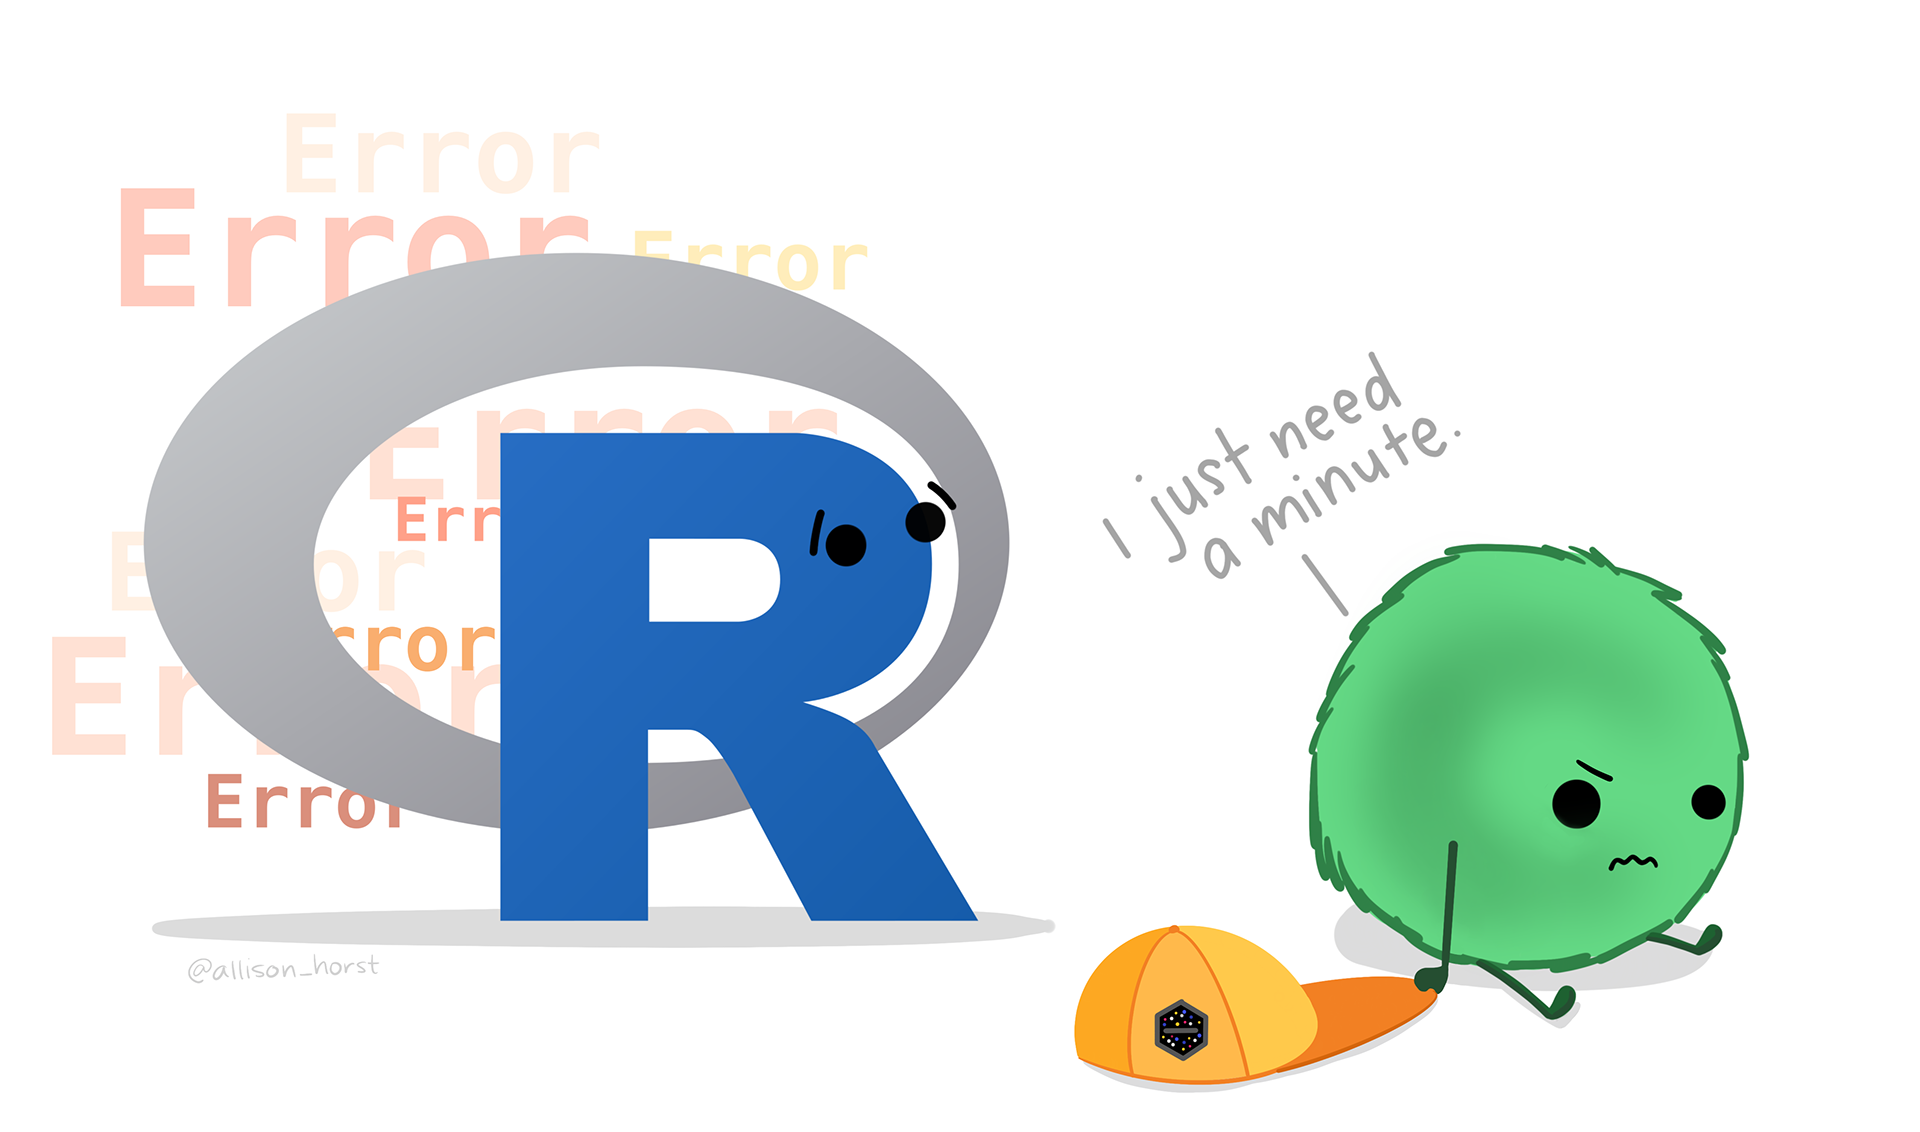
\includegraphics[width=4.6875in,height=\textheight]{images/AHorst_ErrorMonster.png}

}

\caption{\label{fig-ErrorMonster}Debugging is an unavoidable part of
writing code. If you're stuck and starting to feel fustrated, the best
thing you can usually do is to take a short break (artwork by
\href{https://allisonhorst.com/allison-horst}{@allison\_horst}).}

\end{figure}%

\begin{tcolorbox}[enhanced jigsaw, breakable, colbacktitle=quarto-callout-note-color!10!white, bottomtitle=1mm, colframe=quarto-callout-note-color-frame, leftrule=.75mm, bottomrule=.15mm, colback=white, toptitle=1mm, rightrule=.15mm, title=\textcolor{quarto-callout-note-color}{\faInfo}\hspace{0.5em}{Click here for the solutions to Task 1}, coltitle=black, opacityback=0, arc=.35mm, left=2mm, titlerule=0mm, toprule=.15mm, opacitybacktitle=0.6]

\begin{enumerate}
\def\labelenumi{\arabic{enumi}.}
\item
  The first error was
  \texttt{object\ \textquotesingle{}my.favorite.number\textquotesingle{}\ not\ found}.
  This means that the object \texttt{my.favorite.number} is not stored
  in your environment. If you think it is, the problem is most likely
  due to a typo. Here, \texttt{my.favorite.number} uses American English
  spelling, whereas we used British English spelling when we created the
  object. To correct the error, you need to use exactly the same
  spelling as when you created the object.
\item
  The second error is also
  \texttt{object\ \textquotesingle{}Negin\textquotesingle{}\ not\ found}.
  However, here we do not expect an object called \texttt{Negin} to be
  in the environment because what we are actually trying to do is create
  and save a new object called \texttt{Negin-Fav-Word}! The problem is
  that \texttt{R} interprets the hyphens in this object name as
  ``minus'' and therefore tries to find the object \texttt{Negin} in
  order to then subtract \texttt{Fav} and \texttt{Word} from it. To
  correct this error, you need to remove the hyphens or replace them by
  dots.
\item
  The third error is yet another \texttt{object\ not\ found\ error}. It
  is another typo: the correct object name is not in the plural form.
\item
  The fourth error is
  \texttt{Error:\ unexpected\ symbol\ in\ "ömers\_favourite\_\ number"}.
  In addition, \texttt{RStudio} warned us that there were some
  ``unexpected tokens'' in this line of code. The unexpected item is the
  space between \texttt{\_} and \texttt{number}. To fix this error, you
  need to remove this space character.
\item
  The object \texttt{my.favourite..number} is not found because the name
  of the object saved in the environment does not have two consecutive
  dots. Note that the error does \emph{not} come from the fact that this
  line begins with some white space and includes multiple space
  characters after the \texttt{=} sign. These added spaces make the line
  more difficult for us humans to read, but \texttt{R} simply ignores
  them. Hence, to fix this error, what you need to do is remove one of
  the consecutive dots in the object name. It is also worth noting that
  this line replaces the value originally stored in
  \texttt{ömers\_favorite\_number} with the value stored in
  \texttt{my.favourite.number}. If you check your environment pane, you
  will see that, once you have corrected the double dot, this line will
  change \texttt{ömers\_favorite\_number} to \texttt{13} - with no
  warning! In other words, here, the equal sign \texttt{=} behaves in
  the same way as the assignment operator \texttt{\textless{}-}.
\item
  If you tried to run this line, you will have noticed that it does not
  actually generate an error. However, you may have noticed that the
  assignment operator is in the opposite direction. This means that
  \texttt{my.favourite.number} is multiplied by two and that this number
  is then assigned to a new object called \texttt{half.my.fav.number}.
  With this in mind, you will likely want to amend the line for the
  outcome to make mathematical sense (or rename the object).
\item
  Running this line will have caused you to run into a \texttt{+}
  situation in the console. As explained earlier in this chapter, to get
  out of it, you should first take your mouse cursor to the Console pane
  and then press ``esc'' on your keyboard to cancel this erroneous line.
  Whilst there is no error message to help you understand where the
  problem is coming from, \texttt{RStudio} helpfully displays a red
  cross icon to the left of the line; hovering over it displays a
  multi-line message. The first line is the relevant one:
  \texttt{unexpected\ token\ \textquotesingle{}s.favourite.number\ \textless{}-\ 5}.
  This tells us that apostrophes are forbidden in object names. Remove
  the \texttt{\textquotesingle{}} and the error will be fixed.
\item
  This line also causes a \texttt{+} situation. In this case, it is due
  to a missing quotation mark. To fix this error, first cancel the
  incomplete line of code by escaping it. Then, add the missing double
  quotation mark in your script and rerun the completed line.
\item
  The message \texttt{Error:\ unexpected\ symbol\ in\ "2FavNumbers"} is
  due to the fact that object names cannot start with a number. Change
  the object name to something like \texttt{TwoFavNumbers} or
  \texttt{Fav2Numbers} to fix the error.
\item
  Here, too, the error message reads \texttt{unexpected\ symbol}.
  However, it is important to remember that the unexpected symbol is not
  within the character string, but rather within the command to assign
  the string to the object name \texttt{good.luck}. Hence, the problem
  is not that this string is in Persian, but rather that one of the
  quotation marks is missing. You can fix the error by ensuring that the
  phrase is enclosed in quotation marks.
\end{enumerate}

\end{tcolorbox}

\bookmarksetup{startatroot}

\chapter*{References}\label{references}
\addcontentsline{toc}{chapter}{References}

\markboth{References}{References}

\phantomsection\label{refs}
\begin{CSLReferences}{1}{0}
\bibitem[\citeproctext]{ref-LibreOffice2024}
2024. LibreOffice. \emph{Wikipedia}.
\url{https://en.wikipedia.org/w/index.php?title=LibreOffice&oldid=1218520104}.

\bibitem[\citeproctext]{ref-parsonsCommunitysourcedGlossaryOpen2022}
Parsons, Sam, Flávio Azevedo, Mahmoud M. Elsherif, Samuel Guay, Owen N.
Shahim, Gisela H. Govaart, Emma Norris, et al. 2022. A community-sourced
glossary of open scholarship terms. \emph{Nature Human Behaviour}.
Nature 6(3). 312--318. \url{https://doi.org/10.1038/s41562-021-01269-4}.

\bibitem[\citeproctext]{ref-rcoreteamLanguageEnvironmentStatistical2024}
R Core Team. 2024. \emph{R: A language and environment for statistical
computing}. R Foundation for Statistical Computing.
\url{https://www.R-project.org/}.

\bibitem[\citeproctext]{ref-silgeJaneaustenrJaneAusten2022}
Silge, Julia. 2022. \emph{Janeaustenr: Jane austen's complete novels}.
\url{https://CRAN.R-project.org/package=janeaustenr}.

\bibitem[\citeproctext]{ref-WinterStatisticsLinguistsIntroduction2019}
Winter, Bodo. 2019. \emph{Statistics for linguists: An introduction
using r}. Routledge. \url{https://doi.org/10.4324/9781315165547}.

\end{CSLReferences}

\cleardoublepage
\phantomsection
\addcontentsline{toc}{part}{Appendices}
\appendix

\chapter{Next-step resources}\label{next-step-resources}

In the hope that this textbook has inspired you to dive deeper into the
wonderful world of quantitative data analysis, statistics, data
visualisation, and coding in R, here is a (work-in-progress) curated
list of further resources to continue your learning journey! 🚀✨

\section{Recommended resources specific to the language
sciences}\label{recommended-resources-specific-to-the-language-sciences}

\begin{itemize}
\item
  Brezina, Vaclav. 2018. Statistics in Corpus Linguistics: A Practical
  Guide. Cambridge: Cambridge University Press.
  https://doi.org/10.1017/9781316410899.
\item
  Desagulier, Guillaume. 2017. Corpus Linguistics and Statistics with R:
  Introduction to Quantitative Methods in Linguistics (Quantitative
  Methods in the Humanities and Social Sciences). Cham: Springer
  International Publishing.
\item
  Gries, Stefan Thomas. 2013. Statistics for linguistics with R: a
  practical introduction. 2nd revised edition. Berlin: De Gruyter
  Mouton.
\item
  LADAL contributors. Tutorials of the Language Technology and Data
  Analysis Laboratory. \url{https://ladal.edu.au/tutorials.html}
  \texttt{Open\ Educational\ Resource}.
\item
  Levshina, Natalia. 2015. How to do linguistics with R: Data
  exploration and statistical analysis. Amsterdam: John Benjamins.
\item
  Schneider, Dr Gerold \& Max Lauber. 2020. Statistics for Linguists.
  \url{https://dlf.uzh.ch/openbooks/statisticsforlinguists/}
  \texttt{Open\ Educational\ Resource}.
\item
  Winter, Bodo. 2019. Statistics for Linguists: An Introduction Using R.
  New York: Routledge.
  \href{https://doi.org/10.1017/9781316410899}{https://doi.org/10.4324/9781315165547}.
\end{itemize}

\section{Further Open Educational Resources (in no particular
order)}\label{further-open-educational-resources-in-no-particular-order}

\begin{itemize}
\tightlist
\item
  Diez, David, Mine Cetinkaya-Rundel, Christopher Barr \& OpenIntro.
  2015. OpenIntro Statistics. Leanpub. \url{https://leanpub.next/os}.
\item
  Guide to Effect Sizes and Confidence Intervals:
  \url{https://matthewbjane.quarto.pub/guide-to-effect-sizes-and-confidence-intervals/}
\item
  Happy Git and GitHub for the useR: \url{https://happygitwithr.com/}
\item
  Quarto \& reproducibility:
  \url{https://ucsbcarpentry.github.io/Reproducible-Publications-with-RStudio-Quarto/index.html}
\item
  Modern Data Visualization with R:
  \url{https://rkabacoff.github.io/datavis}
\item
  Building reproducible analytical pipelines with R:
  \url{https://raps-with-r.dev/}
\item
  Modern Plain Text Computing:
  \url{https://mptc.io/content/01-content.html}
\item
  \url{https://www.data-to-viz.com/}
\item
  Interpreting data visualisation:
  \url{https://pressbooks.library.torontomu.ca/criticaldataliteracy/}
\item
  Improve your statistical inferences:
  \url{https://lakens.github.io/statistical_inferences/}
\item
  What they forgot to teach you about R: \url{https://rstats.wtf/}
\item
  Introduction to Data Science:
  \url{https://florian-huber.github.io/data_science_course/book/cover.html}
\item
  Data Science in Education Using R:
  \url{https://datascienceineducation.com/}
\item
  Models Demystified: A Practical Guide from t-tests to Deep Learning
  \url{https://m-clark.github.io/book-of-models/}
\item
  Data Visualization in R
  \url{https://datavizf23.classes.andrewheiss.com/}
\item
  R for Data Science \url{https://r4ds.hadley.nz/intro}
\end{itemize}



\end{document}
